% \part{Tutorials and Guidelines}
\part{教程和指导}

{\Large \emph{by Till Tantau}}

\bigskip
\noindent
% To help you get started with \tikzname, instead of a long installation
% and configuration section, this manual starts with tutorials. They
% explain all the basic and some of the more advanced features of the
% system, without going into all the details. This part also contains
% some guidelines on how you should proceed when creating graphics using
% \tikzname.
为了帮你入门 \tikzname,本手册没有立刻给出长长的安装和配置过程,而是直接从教程开始。
这些教程解释了该系统所有基本特性和部分高级特性,并不深入所有细节。
这部分还指导你在用 \tikzname 绘图时,如何继续前进。

\vskip3cm

\begin{codeexample}[graphic=white,width=0pt]
\tikz \draw[thick,rounded corners=8pt]
  (0,0) -- (0,2) -- (1,3.25) -- (2,2) -- (2,0) -- (0,2) -- (2,2) -- (0,0) -- (2,0);
\end{codeexample}

\clearpage
% % Copyright 2006 by Till Tantau
%
% This file may be distributed and/or modified
%
% 1. under the LaTeX Project Public License and/or
% 2. under the GNU Free Documentation License.
%
% See the file doc/generic/pgf/licenses/LICENSE for more details.


\section{Tutorial: A Picture for Karl's Students}

This tutorial is intended for new users of \tikzname. It does not give an
exhaustive account of all the features of \tikzname, just of those that you are
likely to use right away.

Karl is a math and chemistry high-school teacher. He used to create the
graphics in his worksheets and exams using \LaTeX's |{picture}| environment.
While the results were acceptable, creating the graphics often turned out to be
a lengthy process. Also, there tended to be problems with lines having slightly
wrong angles and circles also seemed to be hard to get right. Naturally, his
students could not care less whether the lines had the exact right angles and
they find Karl's exams too difficult no matter how nicely they were drawn. But
Karl was never entirely satisfied with the result.

Karl's son, who was even less satisfied with the results (he did not have to
take the exams, after all), told Karl that he might wish to try out a new
package for creating graphics. A bit confusingly, this package seems to have
two names: First, Karl had to download and install a package called \pgfname.
Then it turns out that inside this package there is another package called
\tikzname, which is supposed to stand for ``\tikzname\ ist \emph{kein}
Zeichenprogramm''. Karl finds this all a bit strange and \tikzname\ seems to
indicate that the package does not do what he needs. However, having used
\textsc{gnu} software for quite some time and ``\textsc{gnu} not being Unix'',
there seems to be hope yet. His son assures him that \tikzname's name is
intended to warn people that \tikzname\ is not a program that you can use to
draw graphics with your mouse or tablet. Rather, it is more like a ``graphics
language''.


\subsection{Problem Statement}

Karl wants to put a graphic on the next worksheet for his students. He is
currently teaching his students about sine and cosine. What he would like to
have is something that looks like this (ideally):
%
\noindent
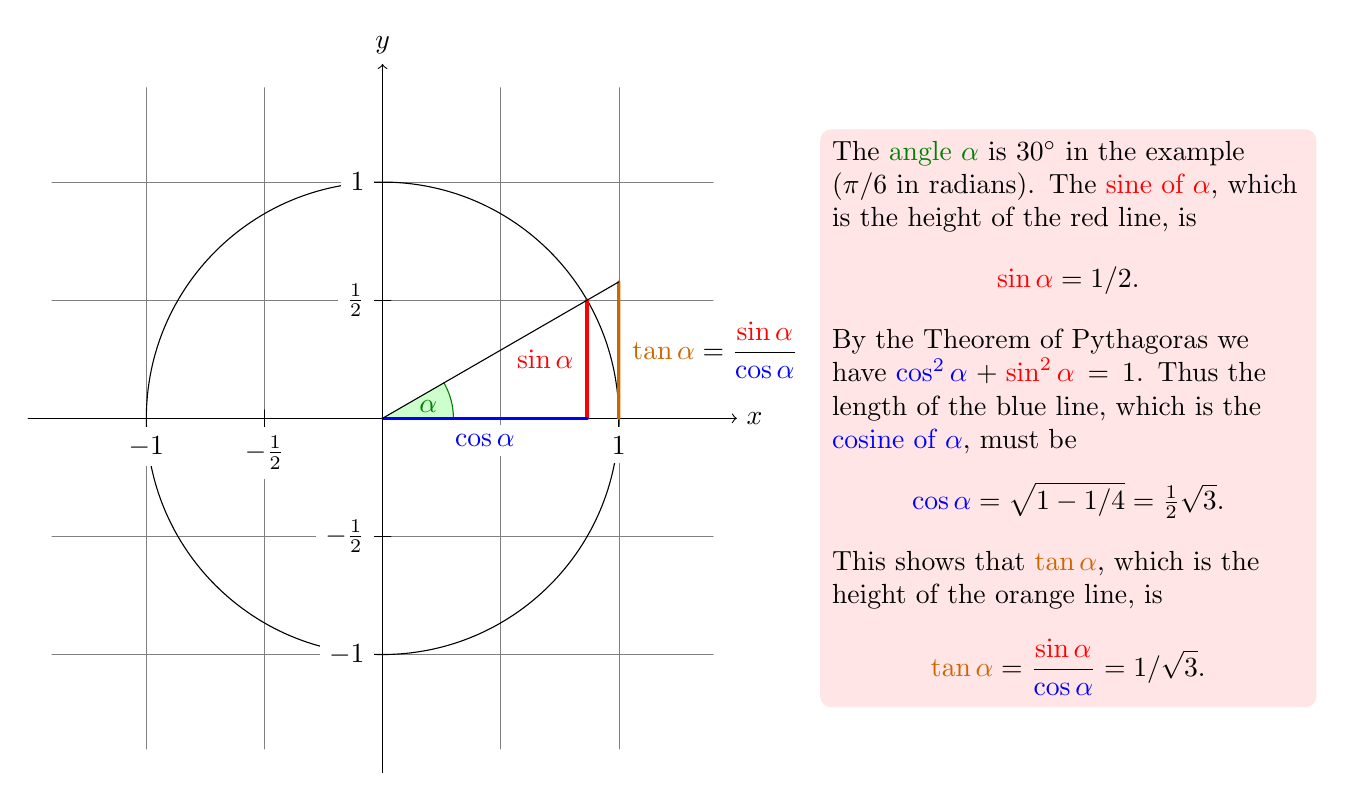
\begin{tikzpicture}
  [scale=3,line cap=round,
   % Styles
   axes/.style=,
   important line/.style={very thick},
   information text/.style={rounded corners,fill=red!10,inner sep=1ex}]

  % Local definitions
  \def\costhirty{0.8660256}

  % Colors
  \colorlet{anglecolor}{green!50!black}
  \colorlet{sincolor}{red}
  \colorlet{tancolor}{orange!80!black}
  \colorlet{coscolor}{blue}

  % The graphic
  \draw[help lines,step=0.5cm] (-1.4,-1.4) grid (1.4,1.4);

  \draw (0,0) circle [radius=1cm];

  \begin{scope}[axes]
    \draw[->] (-1.5,0) -- (1.5,0) node[right] {$x$};
    \draw[->] (0,-1.5) -- (0,1.5) node[above] {$y$};

    \foreach \x/\xtext in {-1, -.5/-\frac{1}{2}, 1}
      \draw[xshift=\x cm] (0pt,1pt) -- (0pt,-1pt) node[below,fill=white] {$\xtext$};

    \foreach \y/\ytext in {-1, -.5/-\frac{1}{2}, .5/\frac{1}{2}, 1}
      \draw[yshift=\y cm] (1pt,0pt) -- (-1pt,0pt) node[left,fill=white] {$\ytext$};
  \end{scope}

  \filldraw[fill=green!20,draw=anglecolor] (0,0) -- (3mm,0pt) arc(0:30:3mm);
  \draw (15:2mm) node[anglecolor] {$\alpha$};

  \draw[important line,sincolor]
    (30:1cm) -- node[left=1pt,fill=white] {$\sin \alpha$} +(0,-.5);

  \draw[important line,coscolor]
    (0,0) -- node[below=2pt,fill=white] {$\cos \alpha$} (\costhirty,0);

  \draw[important line,tancolor] (1,0) --
    node [right=1pt,fill=white]
    {
      $\displaystyle \tan \alpha \color{black}=
      \frac{{\color{sincolor}\sin \alpha}}{\color{coscolor}\cos \alpha}$
    } (intersection of 0,0--30:1cm and 1,0--1,1) coordinate (t);

  \draw (0,0) -- (t);

  \draw[xshift=1.85cm] node [right,text width=6cm,information text]
    {
      The {\color{anglecolor} angle $\alpha$} is $30^\circ$ in the
      example ($\pi/6$ in radians). The {\color{sincolor}sine of
        $\alpha$}, which is the height of the red line, is
      \[
      {\color{sincolor} \sin \alpha} = 1/2.
      \]
      By the Theorem of Pythagoras we have ${\color{coscolor}\cos^2 \alpha} +
      {\color{sincolor}\sin^2\alpha} =1$. Thus the length of the blue
      line, which is the {\color{coscolor}cosine of $\alpha$}, must be
      \[
      {\color{coscolor}\cos\alpha} = \sqrt{1 - 1/4} = \textstyle
      \frac{1}{2} \sqrt 3.
      \]%
      This shows that {\color{tancolor}$\tan \alpha$}, which is the
      height of the orange line, is
      \[
      {\color{tancolor}\tan\alpha} = \frac{{\color{sincolor}\sin
          \alpha}}{\color{coscolor}\cos \alpha} = 1/\sqrt 3.
      \]%
    };
\end{tikzpicture}


\subsection{Setting up the Environment}

In \tikzname, to draw a picture, at the start of the picture you need to tell
\TeX\ or \LaTeX\ that you want to start a picture. In \LaTeX\ this is done
using the environment |{tikzpicture}|, in plain \TeX\ you just use
|\tikzpicture| to start the picture and |\endtikzpicture| to end it.


\subsubsection{Setting up the Environment in \LaTeX}

Karl, being a \LaTeX\ user, thus sets up his file as follows:
%
\begin{codeexample}[code only]
\documentclass{article} % say
\usepackage{tikz}
\begin{document}
We are working on
\begin{tikzpicture}
  \draw (-1.5,0) -- (1.5,0);
  \draw (0,-1.5) -- (0,1.5);
\end{tikzpicture}.
\end{document}
\end{codeexample}

When executed, that is, run via |pdflatex| or via |latex| followed by |dvips|,
the resulting will contain something that looks like this:
%
\begin{codeexample}[width=7cm]
We are working on
\begin{tikzpicture}
  \draw (-1.5,0) -- (1.5,0);
  \draw (0,-1.5) -- (0,1.5);
\end{tikzpicture}.
\end{codeexample}

Admittedly, not quite the whole picture, yet, but we do have the axes
established. Well, not quite, but we have the lines that make up the axes
drawn. Karl suddenly has a sinking feeling that the picture is still some way
off.

Let's have a more detailed look at the code. First, the package |tikz| is
loaded. This package is a so-called ``frontend'' to the basic \pgfname\ system.
The basic layer, which is also described in this manual, is somewhat more,
well, basic and thus harder to use. The frontend makes things easier by
providing a simpler syntax.

Inside the environment there are two |\draw| commands. They mean: ``The path,
which is specified following the command up to the semicolon, should be
drawn.'' The first path is specified as |(-1.5,0) -- (0,1.5)|, which means ``a
straight line from the point at position $(-1.5,0)$ to the point at position
$(0,1.5)$''. Here, the positions are specified within a special coordinate
system in which, initially, one unit is 1cm.

Karl is quite pleased to note that the environment automatically reserves
enough space to encompass the picture.


\subsubsection{Setting up the Environment in Plain \TeX}

Karl's wife Gerda, who also happens to be a math teacher, is not a \LaTeX\
user, but uses plain \TeX\ since she prefers to do things ``the old way''. She
can also use \tikzname. Instead of |\usepackage{tikz}| she has to write
|\input tikz.tex| and instead of |\begin{tikzpicture}| she writes
|\tikzpicture| and instead of |\end{tikzpicture}| she writes |\endtikzpicture|.

Thus, she would use:
%
\begin{codeexample}[code only]
%% Plain TeX file
\input tikz.tex
\baselineskip=12pt
\hsize=6.3truein
\vsize=8.7truein
We are working on
\tikzpicture
  \draw (-1.5,0) -- (1.5,0);
  \draw (0,-1.5) -- (0,1.5);
\endtikzpicture.
\bye
\end{codeexample}

Gerda can typeset this file using either |pdftex| or |tex| together with
|dvips|. \tikzname\ will automatically discern which driver she is using. If
she wishes to use |dvipdfm| together with |tex|, she either needs to modify the
file |pgf.cfg| or can write |\def\pgfsysdriver{pgfsys-dvipdfm.def}| somewhere
\emph{before} she inputs |tikz.tex| or |pgf.tex|.


\subsubsection{Setting up the Environment in Con\TeX t}

Karl's uncle Hans uses Con\TeX t. Like Gerda, Hans can also use \tikzname.
Instead of |\usepackage{tikz}| he says |\usemodule[tikz]|. Instead of
|\begin{tikzpicture}| he writes |\starttikzpicture| and  instead of
|\end{tikzpicture}| he writes |\stoptikzpicture|.

His version of the example looks like this:
%
\begin{codeexample}[code only]
%% ConTeXt file
\usemodule[tikz]

\starttext
  We are working on
  \starttikzpicture
    \draw (-1.5,0) -- (1.5,0);
    \draw (0,-1.5) -- (0,1.5);
  \stoptikzpicture.
\stoptext
\end{codeexample}

Hans will now typeset this file in the usual way using |texexec| or |context|.


\subsection{Straight Path Construction}

The basic building block of all pictures in \tikzname\ is the path. A
\emph{path} is a series of straight lines and curves that are connected (that
is not the whole picture, but let us ignore the complications for the moment).
You start a path by specifying the coordinates of the start position as a point
in round brackets, as in |(0,0)|. This is followed by a series of ``path
extension operations''. The simplest is |--|, which we used already. It must be
followed by another coordinate and it extends the path in a straight line to
this new position. For example, if we were to turn the two paths of the axes
into one path, the following would result:
%
\begin{codeexample}[]
\tikz \draw (-1.5,0) -- (1.5,0) -- (0,-1.5) -- (0,1.5);
\end{codeexample}

Karl is a bit confused by the fact that there is no |{tikzpicture}|
environment, here. Instead, the little command |\tikz| is used. This command
either takes one argument (starting with an opening brace as in
|\tikz{\draw (0,0) -- (1.5,0)}|, which yields \tikz{\draw (0,0) --(1.5,0);}) or
collects everything up to the next semicolon and puts it inside a
|{tikzpicture}| environment. As a rule of thumb, all \tikzname\ graphic drawing
commands must occur as an argument of |\tikz| or inside a |{tikzpicture}|
environment. Fortunately, the command |\draw| will only be defined inside this
environment, so there is little chance that you will accidentally do something
wrong here.


\subsection{Curved Path Construction}

The next thing Karl wants to do is to draw the circle. For this, straight lines
obviously will not do. Instead, we need some way to draw curves. For this,
\tikzname\ provides a special syntax. One or two ``control points'' are needed.
The math behind them is not quite trivial, but here is the basic idea: Suppose
you are at point $x$ and the first control point is $y$. Then the curve will
start ``going in the direction of~$y$ at~$x$'', that is, the tangent of the
curve at $x$ will point toward~$y$. Next, suppose the curve should end at $z$
and the second support point is $w$. Then the curve will, indeed, end at $z$
and the tangent of the curve at point $z$ will go through $w$.

Here is an example (the control points have been added for clarity):
%
\begin{codeexample}[]
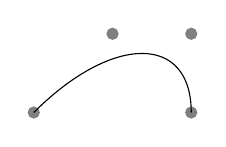
\begin{tikzpicture}
  \filldraw [gray] (0,0) circle [radius=2pt]
                   (1,1) circle [radius=2pt]
                   (2,1) circle [radius=2pt]
                   (2,0) circle [radius=2pt];
  \draw (0,0) .. controls (1,1) and (2,1) .. (2,0);
\end{tikzpicture}
\end{codeexample}

The general syntax for extending a path in a ``curved'' way is |.. controls|
\meta{first control point} |and| \meta{second control point} |..|
\meta{end point}. You can leave out the |and| \meta{second control point},
which causes the first one to be used twice.

So, Karl can now add the first half circle to the picture:
%
\begin{codeexample}[]
\begin{tikzpicture}
  \draw (-1.5,0) -- (1.5,0);
  \draw (0,-1.5) -- (0,1.5);
  \draw (-1,0) .. controls (-1,0.555) and (-0.555,1) .. (0,1)
               .. controls (0.555,1) and (1,0.555) .. (1,0);
\end{tikzpicture}
\end{codeexample}

Karl is happy with the result, but finds specifying circles in this way to be
extremely awkward. Fortunately, there is a much simpler way.


\subsection{Circle Path Construction}

In order to draw a circle, the path construction operation |circle| can be
used. This operation is followed by a radius in brackets as in the following
example: (Note that the previous position is used as the \emph{center} of the
circle.)
%
\begin{codeexample}[]
\tikz \draw (0,0) circle [radius=10pt];
\end{codeexample}

You can also append an ellipse to the path using the |ellipse| operation.
Instead of a single radius you can specify two of them:
%
\begin{codeexample}[]
\tikz \draw (0,0) ellipse [x radius=20pt, y radius=10pt];
\end{codeexample}

To draw an ellipse whose axes are not horizontal and vertical, but point in an
arbitrary direction (a ``turned ellipse'' like \tikz \draw[rotate=30] (0,0)
ellipse [x radius=6pt, y radius=3pt];) you can use transformations, which are
explained later. The code for the little ellipse is
|\tikz \draw[rotate=30] (0,0) ellipse [x radius=6pt, y radius=3pt];|, by the
way.

So, returning to Karl's problem, he can write
|\draw (0,0) circle [radius=1cm];| to draw the circle:
%
\begin{codeexample}[]
\begin{tikzpicture}
  \draw (-1.5,0) -- (1.5,0);
  \draw (0,-1.5) -- (0,1.5);
  \draw (0,0) circle [radius=1cm];
\end{tikzpicture}
\end{codeexample}

At this point, Karl is a bit alarmed that the circle is so small when he wants
the final picture to be much bigger. He is pleased to learn that \tikzname\ has
powerful transformation options and scaling everything by a factor of three is
very easy. But let us leave the size as it is for the moment to save some
space.


\subsection{Rectangle Path Construction}

The next things we would like to have is the grid in the background. There are
several ways to produce it. For example, one might draw lots of rectangles.
Since rectangles are so common, there is a special syntax for them: To add a
rectangle to the current path, use the |rectangle| path construction operation.
This operation should be followed by another coordinate and will append a
rectangle to the path such that the previous coordinate and the next
coordinates are corners of the rectangle. So, let us add two rectangles to the
picture:
%
\begin{codeexample}[]
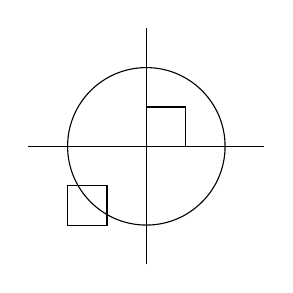
\begin{tikzpicture}
  \draw (-1.5,0) -- (1.5,0);
  \draw (0,-1.5) -- (0,1.5);
  \draw (0,0) circle [radius=1cm];
  \draw (0,0) rectangle (0.5,0.5);
  \draw (-0.5,-0.5) rectangle (-1,-1);
\end{tikzpicture}
\end{codeexample}

While this may be nice in other situations, this is not really leading anywhere
with Karl's problem: First, we would need an awful lot of these rectangles and
then there is the border that is not ``closed''.

So, Karl is about to resort to simply drawing four vertical and four horizontal
lines using the nice |\draw| command, when he learns that there is a |grid|
path construction operation.


\subsection{Grid Path Construction}

The |grid| path operation adds a grid to the current path. It will add lines
making up a grid that fills the rectangle whose one corner is the current point
and whose other corner is the point following the |grid| operation. For
example, the code |\tikz \draw[step=2pt] (0,0) grid (10pt,10pt);| produces
\tikz \draw[step=2pt] (0,0) grid (10pt,10pt);. Note how the optional argument
for |\draw| can be used to specify a grid width (there are also |xstep| and
|ystep| to define the steppings independently). As Karl will learn soon, there
are \emph{lots} of things that can be influenced using such options.

For Karl, the following code could be used:
%
\begin{codeexample}[]
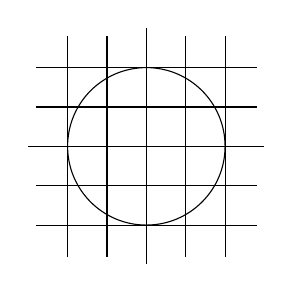
\begin{tikzpicture}
  \draw (-1.5,0) -- (1.5,0);
  \draw (0,-1.5) -- (0,1.5);
  \draw (0,0) circle [radius=1cm];
  \draw[step=.5cm] (-1.4,-1.4) grid (1.4,1.4);
\end{tikzpicture}
\end{codeexample}

Having another look at the desired picture, Karl notices that it would be nice
for the grid to be more subdued. (His son told him that grids tend to be
distracting if they are not subdued.) To subdue the grid, Karl adds two more
options to the |\draw| command that draws the grid. First, he uses the color
|gray| for the grid lines. Second, he reduces the line width to |very thin|.
Finally, he swaps the ordering of the commands so that the grid is drawn first
and everything else on top.
%
\begin{codeexample}[]
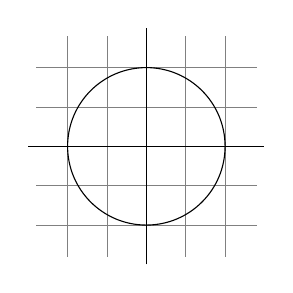
\begin{tikzpicture}
  \draw[step=.5cm,gray,very thin] (-1.4,-1.4) grid (1.4,1.4);
  \draw (-1.5,0) -- (1.5,0);
  \draw (0,-1.5) -- (0,1.5);
  \draw (0,0) circle [radius=1cm];
\end{tikzpicture}
\end{codeexample}


\subsection{Adding a Touch of  Style}

Instead of the options |gray,very thin| Karl could also have said |help lines|.
\emph{Styles} are predefined sets of options that can be used to organize how a
graphic is drawn. By saying |help lines| you say ``use the style that I (or
someone else) has set for drawing help lines''. If Karl decides, at some later
point, that grids should be drawn, say, using the color |blue!50| instead of
|gray|, he could provide the following option somewhere:
%
\begin{codeexample}[code only]
help lines/.style={color=blue!50,very thin}
\end{codeexample}
%
The effect of this ``style setter'' is that in the current scope or environment
the |help lines| option has the same effect as |color=blue!50,very thin|.

Using styles makes your graphics code more flexible. You can change the way
things look easily in a consistent manner. Normally, styles are defined at the
beginning of a picture. However, you may sometimes wish to define a style
globally, so that all pictures of your document can use this style. Then you
can easily change the way all graphics look by changing this one style. In this
situation you can use the |\tikzset| command at the beginning of the document
as in
%
\begin{codeexample}[code only]
\tikzset{help lines/.style=very thin}
\end{codeexample}

To build a hierarchy of styles you can have one style use another. So in order
to define a style |Karl's grid| that is based on the |grid| style Karl could
say
%
\begin{codeexample}[code only]
\tikzset{Karl's grid/.style={help lines,color=blue!50}}
...
\draw[Karl's grid] (0,0) grid (5,5);
\end{codeexample}

Styles are made even more powerful by parametrization. This means that, like
other options, styles can also be used with a parameter. For instance, Karl
could parameterize his grid so that, by default, it is blue, but he could also
use another color.
%
\begin{codeexample}[code only]
\begin{tikzpicture}
  [Karl's grid/.style  ={help lines,color=#1!50},
   Karl's grid/.default=blue]

  \draw[Karl's grid]     (0,0) grid (1.5,2);
  \draw[Karl's grid=red] (2,0) grid (3.5,2);
\end{tikzpicture}
\end{codeexample}

 In this example, the definition of the style |Karl's grid| is given as an
 optional argument to the |{tikzpicture}| environment. Additional styles for other
 elements would follow after a comma. With many styles in effect, the optional
 argument of the environment may easily happen to be longer than the actual
 contents.

\subsection{Drawing Options}

Karl wonders what other options there are that influence how a path is drawn.
He saw already that the |color=|\meta{color} option can be used to set the
line's color. The option |draw=|\meta{color} does nearly the same, only it sets
the color for the lines only and a different color can be used for filling
(Karl will need this when he fills the arc for the angle).

He saw that the style |very thin| yields very thin lines. Karl is not really
surprised by this and neither is he surprised to learn that |thin| yields thin
lines,  |thick| yields thick lines, |very thick| yields very thick lines,
|ultra thick| yields really, really thick lines and |ultra thin| yields lines
that are so thin that low-resolution printers and displays will have trouble
showing them. He wonders what gives lines of ``normal'' thickness. It turns out
that |thin| is the correct choice, since it gives the same thickness as \TeX's
|\hrule| command. Nevertheless, Karl would like to know whether there is
anything ``in the middle'' between |thin| and |thick|. There is: |semithick|.

Another useful thing one can do with lines is to dash or dot them. For this,
the two styles |dashed| and |dotted| can be used, yielding \tikz[baseline]
\draw[dashed] (0,.5ex) -- ++(2em,0pt); and \tikz[baseline] \draw[dotted]
(0,.5ex) -- ++(2em,0pt);. Both options also exist in a loose and a dense
version, called |loosely dashed|, |densely dashed|, |loosely dotted|, and
|densely dotted|. If he really, really  needs to, Karl can also define much
more complex dashing patterns with the |dash pattern| option, but his son
insists that dashing is to be used with utmost care and mostly distracts.
Karl's son claims that complicated dashing patterns are evil. Karl's students
do not care about dashing patterns.


\subsection{Arc Path Construction}

Our next obstacle is to draw the arc for the angle. For this, the |arc| path
construction operation is useful, which draws part of a circle or ellipse. This
|arc| operation is followed by options in brackets that specify the arc. An
example would be \texttt{arc[start angle=10, end angle=80, radius=10pt]}, which
means exactly what it says. Karl obviously needs an arc from $0^\circ$ to
$30^\circ$. The radius should be something relatively small, perhaps around one
third of the circle's radius. When one uses the arc path construction
operation, the specified arc will be added with its starting point at the
current position. So, we first have to ``get there''.
%
\begin{codeexample}[]
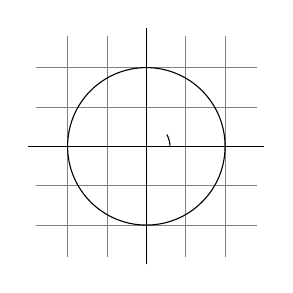
\begin{tikzpicture}
  \draw[step=.5cm,gray,very thin] (-1.4,-1.4) grid (1.4,1.4);
  \draw (-1.5,0) -- (1.5,0);
  \draw (0,-1.5) -- (0,1.5);
  \draw (0,0) circle [radius=1cm];
  \draw (3mm,0mm) arc [start angle=0, end angle=30, radius=3mm];
\end{tikzpicture}
\end{codeexample}

Karl thinks this is really a bit small and he cannot continue unless he learns
how to do scaling. For this, he can add the |[scale=3]| option. He could add
this option to each |\draw| command, but that would be awkward. Instead, he
adds it to the whole environment, which causes this option to apply to
everything within.
%
\begin{codeexample}[]
\begin{tikzpicture}[scale=3]
  \draw[step=.5cm,gray,very thin] (-1.4,-1.4) grid (1.4,1.4);
  \draw (-1.5,0) -- (1.5,0);
  \draw (0,-1.5) -- (0,1.5);
  \draw (0,0) circle [radius=1cm];
  \draw (3mm,0mm) arc [start angle=0, end angle=30, radius=3mm];
\end{tikzpicture}
\end{codeexample}

As for circles, you can specify ``two'' radii in order to get an elliptical
arc.
%
\begin{codeexample}[]
  \tikz \draw (0,0)
    arc [start angle=0, end angle=315,
         x radius=1.75cm, y radius=1cm];
\end{codeexample}


\subsection{Clipping a Path}

In order to save space in this manual, it would be nice to clip Karl's graphics
a bit so that we can focus on the ``interesting'' parts. Clipping is pretty
easy in \tikzname. You can use the |\clip| command to clip all subsequent
drawing. It works like |\draw|, only it does not draw anything, but uses the
given path to clip everything subsequently.
%
\begin{codeexample}[]
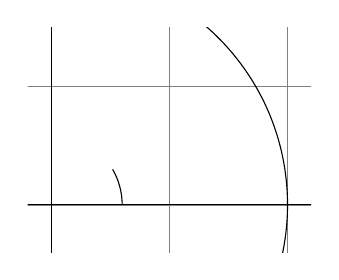
\begin{tikzpicture}[scale=3]
  \clip (-0.1,-0.2) rectangle (1.1,0.75);
  \draw[step=.5cm,gray,very thin] (-1.4,-1.4) grid (1.4,1.4);
  \draw (-1.5,0) -- (1.5,0);
  \draw (0,-1.5) -- (0,1.5);
  \draw (0,0) circle [radius=1cm];
  \draw (3mm,0mm) arc [start angle=0, end angle=30, radius=3mm];
\end{tikzpicture}
\end{codeexample}

You can also do both at the same time: Draw \emph{and} clip a path. For this,
use the |\draw| command and add the |clip| option. (This is not the whole
picture: You can also use the |\clip| command and add the |draw| option. Well,
that is also not the whole picture: In reality, |\draw| is just a shorthand for
|\path[draw]| and |\clip| is a shorthand for |\path[clip]| and you could also
say |\path[draw,clip]|.) Here is an example:
%
\begin{codeexample}[]
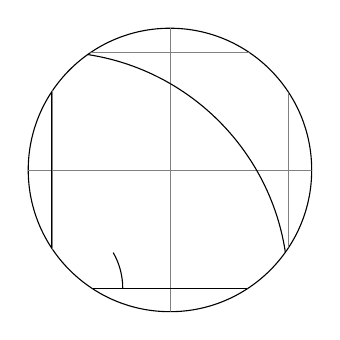
\begin{tikzpicture}[scale=3]
  \clip[draw] (0.5,0.5) circle (.6cm);
  \draw[step=.5cm,gray,very thin] (-1.4,-1.4) grid (1.4,1.4);
  \draw (-1.5,0) -- (1.5,0);
  \draw (0,-1.5) -- (0,1.5);
  \draw (0,0) circle [radius=1cm];
  \draw (3mm,0mm) arc [start angle=0, end angle=30, radius=3mm];
\end{tikzpicture}
\end{codeexample}


\subsection{Parabola and Sine Path Construction}

Although Karl does not need them for his picture, he is pleased to learn that
there are |parabola| and |sin| and |cos| path operations for adding parabolas
and sine and cosine curves to the current path. For the |parabola| operation,
the current point will lie on the parabola as well as the point given after the
parabola operation. Consider the following example:
%
\begin{codeexample}[]
\tikz \draw (0,0) rectangle (1,1)  (0,0) parabola (1,1);
\end{codeexample}

It is also possible to place the bend somewhere else:
%
\begin{codeexample}[]
\tikz \draw[x=1pt,y=1pt] (0,0) parabola bend (4,16) (6,12);
\end{codeexample}

The operations |sin| and |cos| add a sine or cosine curve in the interval
$[0,\pi/2]$ such that the previous current point is at the start of the curve
and the curve ends at the given end point. Here are two examples:
%
\begin{codeexample}[]
A sine \tikz \draw[x=1ex,y=1ex] (0,0) sin (1.57,1); curve.
\end{codeexample}

\begin{codeexample}[]
\tikz \draw[x=1.57ex,y=1ex] (0,0) sin (1,1) cos (2,0) sin (3,-1) cos (4,0)
                            (0,1) cos (1,0) sin (2,-1) cos (3,0) sin (4,1);
\end{codeexample}


\subsection{Filling and Drawing}

Returning to the picture, Karl now wants the angle to be ``filled'' with a very
light green. For this he uses |\fill| instead of |\draw|. Here is what Karl
does:
%
\begin{codeexample}[]
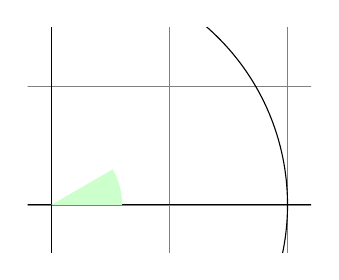
\begin{tikzpicture}[scale=3]
  \clip (-0.1,-0.2) rectangle (1.1,0.75);
  \draw[step=.5cm,gray,very thin] (-1.4,-1.4) grid (1.4,1.4);
  \draw (-1.5,0) -- (1.5,0);
  \draw (0,-1.5) -- (0,1.5);
  \draw (0,0) circle [radius=1cm];
  \fill[green!20!white] (0,0) -- (3mm,0mm)
    arc [start angle=0, end angle=30, radius=3mm] -- (0,0);
\end{tikzpicture}
\end{codeexample}

The color |green!20!white| means 20\% green and 80\% white mixed together. Such
color expression are possible since \tikzname\ uses Uwe Kern's |xcolor|
package, see the documentation of that package for details on color
expressions.

What would have happened, if Karl had not ``closed'' the path using |--(0,0)|
at the end? In this case, the path is closed automatically, so this could have
been omitted. Indeed, it would even have been better to write the following,
instead:
%
\begin{codeexample}[code only]
  \fill[green!20!white] (0,0) -- (3mm,0mm)
    arc [start angle=0, end angle=30, radius=3mm] -- cycle;
\end{codeexample}
%
The |--cycle| causes the current path to be closed (actually the current part
of the current path) by smoothly joining the first and last point. To
appreciate the difference, consider the following example:
%
\begin{codeexample}[]
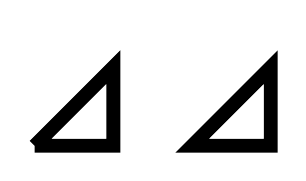
\begin{tikzpicture}[line width=5pt]
  \draw (0,0) -- (1,0) -- (1,1) -- (0,0);
  \draw (2,0) -- (3,0) -- (3,1) -- cycle;
  \useasboundingbox (0,1.5); % make bounding box higher
\end{tikzpicture}
\end{codeexample}

You can also fill and draw a path at the same time using the |\filldraw|
command. This will first draw the path, then fill it. This may not seem too
useful, but you can specify different colors to be used for filling and for
stroking. These are specified as optional arguments like this:
%
\begin{codeexample}[]
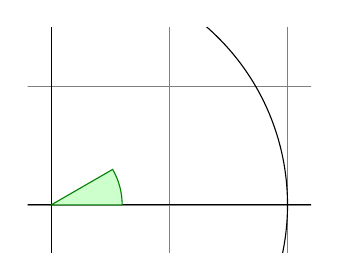
\begin{tikzpicture}[scale=3]
  \clip (-0.1,-0.2) rectangle (1.1,0.75);
  \draw[step=.5cm,gray,very thin] (-1.4,-1.4) grid (1.4,1.4);
  \draw (-1.5,0) -- (1.5,0);
  \draw (0,-1.5) -- (0,1.5);
  \draw (0,0) circle [radius=1cm];
  \filldraw[fill=green!20!white, draw=green!50!black] (0,0) -- (3mm,0mm)
    arc [start angle=0, end angle=30, radius=3mm] -- cycle;
\end{tikzpicture}
\end{codeexample}


\subsection{Shading}

Karl briefly considers the possibility of making the angle ``more fancy'' by
\emph{shading} it. Instead of filling the area with a uniform color, a smooth
transition between different colors is used. For this, |\shade| and
|\shadedraw|, for shading and drawing at the same time, can be used:
%
\begin{codeexample}[]
  \tikz \shade (0,0) rectangle (2,1)  (3,0.5) circle (.5cm);
\end{codeexample}
%
The default shading is a smooth transition from gray to white. To specify
different colors, you can use options:
%
\begin{codeexample}[]

\begin{tikzpicture}[rounded corners,ultra thick]
  \shade[top color=yellow,bottom color=black] (0,0) rectangle +(2,1);
  \shade[left color=yellow,right color=black] (3,0) rectangle +(2,1);
  \shadedraw[inner color=yellow,outer color=black,draw=yellow] (6,0) rectangle +(2,1);
  \shade[ball color=green] (9,.5) circle (.5cm);
\end{tikzpicture}
\end{codeexample}

For Karl, the following might be appropriate:
%
\begin{codeexample}[]
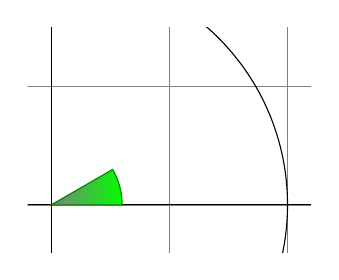
\begin{tikzpicture}[scale=3]
  \clip (-0.1,-0.2) rectangle (1.1,0.75);
  \draw[step=.5cm,gray,very thin] (-1.4,-1.4) grid (1.4,1.4);
  \draw (-1.5,0) -- (1.5,0);
  \draw (0,-1.5) -- (0,1.5);
  \draw (0,0) circle [radius=1cm];
  \shadedraw[left color=gray,right color=green, draw=green!50!black]
    (0,0) -- (3mm,0mm)
    arc [start angle=0, end angle=30, radius=3mm] -- cycle;
\end{tikzpicture}
\end{codeexample}

However, he wisely decides that shadings usually only distract without adding
anything to the picture.


\subsection{Specifying Coordinates}

Karl now wants to add the sine and cosine lines. He knows already that he can
use the |color=| option to set the lines' colors. So, what is the best way to
specify the coordinates?

There are different ways of specifying coordinates. The easiest way is to say
something like |(10pt,2cm)|. This means 10pt in $x$-direction and 2cm in
$y$-directions. Alternatively, you can also leave out the units as in |(1,2)|,
which means ``one times the current $x$-vector plus twice the current
$y$-vector''. These vectors default to 1cm in the $x$-direction and 1cm in the
$y$-direction, respectively.

In order to specify points in polar coordinates, use the notation |(30:1cm)|,
which means 1cm in direction 30 degree. This is obviously quite useful to ``get
to the point $(\cos 30^\circ,\sin 30^\circ)$ on the circle''.

You can add a single |+| sign in front of a coordinate or two of them as in
|+(0cm,1cm)| or |++(2cm,0cm)|. Such coordinates are interpreted differently:
The first form means ``1cm upwards from the previous specified position'' and
the second means ``2cm to the right of the previous specified position, making
this the new specified position''. For example, we can draw the sine line as
follows:
%
\begin{codeexample}[]
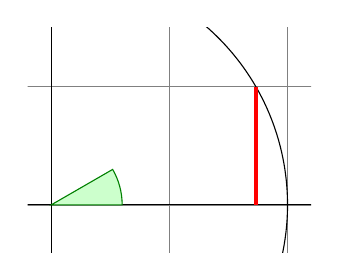
\begin{tikzpicture}[scale=3]
  \clip (-0.1,-0.2) rectangle (1.1,0.75);
  \draw[step=.5cm,gray,very thin] (-1.4,-1.4) grid (1.4,1.4);
  \draw (-1.5,0) -- (1.5,0);
  \draw (0,-1.5) -- (0,1.5);
  \draw (0,0) circle [radius=1cm];
  \filldraw[fill=green!20,draw=green!50!black] (0,0) -- (3mm,0mm)
      arc [start angle=0, end angle=30, radius=3mm] -- cycle;
  \draw[red,very thick] (30:1cm) -- +(0,-0.5);
\end{tikzpicture}
\end{codeexample}

Karl used the fact $\sin 30^\circ = 1/2$. However, he very much doubts that his
students know this, so it would be nice to have a way of specifying ``the point
straight down from |(30:1cm)| that lies on the $x$-axis''. This is, indeed,
possible using a special syntax: Karl can write \verb!(30:1cm |- 0,0)!. In
general, the meaning of |(|\meta{p}\verb! |- !\meta{q}|)| is ``the intersection
of a vertical line through $p$ and a horizontal line through $q$''.

Next, let us draw the cosine line. One way would be to say
\verb!(30:1cm |- 0,0) -- (0,0)!. Another way is the following: we ``continue''
from where the sine ends:
%
\begin{codeexample}[]
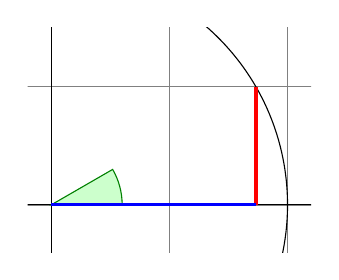
\begin{tikzpicture}[scale=3]
  \clip (-0.1,-0.2) rectangle (1.1,0.75);
  \draw[step=.5cm,gray,very thin] (-1.4,-1.4) grid (1.4,1.4);
  \draw (-1.5,0) -- (1.5,0);
  \draw (0,-1.5) -- (0,1.5);
  \draw (0,0) circle [radius=1cm];
  \filldraw[fill=green!20,draw=green!50!black] (0,0) -- (3mm,0mm)
      arc [start angle=0, end angle=30, radius=3mm] -- cycle;
  \draw[red,very thick]  (30:1cm) -- +(0,-0.5);
  \draw[blue,very thick] (30:1cm) ++(0,-0.5) -- (0,0);
\end{tikzpicture}
\end{codeexample}

Note that there is no |--| between |(30:1cm)| and |++(0,-0.5)|. In detail, this
path is interpreted as follows: ``First, the |(30:1cm)| tells me to move by pen
to $(\cos 30^\circ,1/2)$. Next, there comes another coordinate specification,
so I move my pen there without drawing anything. This new point is half a unit
down from the last position, thus it is at $(\cos 30^\circ,0)$. Finally, I move
the pen to the origin, but this time drawing something (because of the |--|).''

To appreciate the difference between |+| and |++| consider the following
example:
%
\begin{codeexample}[]
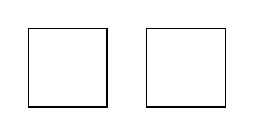
\begin{tikzpicture}
  \def\rectanglepath{-- ++(1cm,0cm)  -- ++(0cm,1cm)  -- ++(-1cm,0cm) -- cycle}
  \draw (0,0) \rectanglepath;
  \draw (1.5,0) \rectanglepath;
\end{tikzpicture}
\end{codeexample}

By comparison, when using a single |+|, the coordinates are different:
%
\begin{codeexample}[]
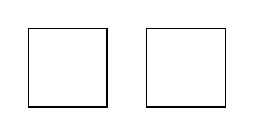
\begin{tikzpicture}
  \def\rectanglepath{-- +(1cm,0cm)  -- +(1cm,1cm)  -- +(0cm,1cm) -- cycle}
  \draw (0,0) \rectanglepath;
  \draw (1.5,0) \rectanglepath;
\end{tikzpicture}
\end{codeexample}


Naturally, all of this could have been written more clearly and more
economically like this (either with a single of a double |+|):
%
\begin{codeexample}[]
\tikz \draw (0,0) rectangle +(1,1)  (1.5,0) rectangle +(1,1);
\end{codeexample}


\subsection{Intersecting Paths}

Karl is left with the line for $\tan \alpha$, which seems difficult to specify
using transformations and polar coordinates. The first -- and easiest -- thing
he can do is so simply use the coordinate |(1,{tan(30)})| since \tikzname's
math engine knows how to compute things like |tan(30)|. Note the added braces
since, otherwise, \tikzname's parser would think that the first closing
parenthesis ends the coordinate (in general, you need to add braces around
components of coordinates when these components contain parentheses).

Karl can, however, also use a more elaborate, but also more ``geometric'' way
of computing the length of the orange line: He can specify intersections of
paths as coordinates. The line for $\tan \alpha$ starts at $(1,0)$ and goes
upward to a point that is at the intersection of a line going ``up'' and a line
going from the origin through |(30:1cm)|. Such computations are made available
by the |intersections| library.

What Karl must do is to create two ``invisible'' paths that intersect at the
position of interest. Creating paths that are not otherwise seen can be done
using the |\path| command without any options like |draw| or |fill|. Then, Karl
can add the |name path| option to the path for later reference. Once the paths
have been constructed, Karl can use the |name intersections| to assign names to
the coordinate for later reference.
%
\begin{codeexample}[code only]
\path [name path=upward line] (1,0) -- (1,1);
\path [name path=sloped line] (0,0) -- (30:1.5cm); % a bit longer, so that there is an intersection

% (add `\usetikzlibrary{intersections}' after loading tikz in the preamble)
\draw [name intersections={of=upward line and sloped line, by=x}]
  [very thick,orange] (1,0) -- (x);
\end{codeexample}


\subsection{Adding Arrow Tips}

Karl now wants to add the little arrow tips at the end of the axes. He has
noticed that in many plots, even in scientific journals, these arrow tips seem
to be missing, presumably because the generating programs cannot produce them.
Karl thinks arrow tips belong at the end of axes. His son agrees. His students
do not care about arrow tips.

It turns out that adding arrow tips is pretty easy: Karl adds the option |->|
to the drawing commands for the axes:
%
\begin{codeexample}[preamble={\usetikzlibrary{intersections}}]
\begin{tikzpicture}[scale=3]
  \clip (-0.1,-0.2) rectangle (1.1,1.51);
  \draw[step=.5cm,gray,very thin] (-1.4,-1.4) grid (1.4,1.4);
  \draw[->] (-1.5,0) -- (1.5,0);
  \draw[->] (0,-1.5) -- (0,1.5);
  \draw (0,0) circle [radius=1cm];
  \filldraw[fill=green!20,draw=green!50!black] (0,0) -- (3mm,0mm)
        arc [start angle=0, end angle=30, radius=3mm] -- cycle;
  \draw[red,very thick]    (30:1cm) -- +(0,-0.5);
  \draw[blue,very thick]   (30:1cm) ++(0,-0.5) -- (0,0);

  \path [name path=upward line] (1,0) -- (1,1);
  \path [name path=sloped line] (0,0) -- (30:1.5cm);
  \draw [name intersections={of=upward line and sloped line, by=x}]
        [very thick,orange] (1,0) -- (x);
\end{tikzpicture}
\end{codeexample}

If Karl had used the option |<-| instead of |->|, arrow tips would have been
put at the beginning of the path. The option |<->| puts arrow tips at both ends
of the path.

There are certain restrictions to the kind of paths to which arrow tips can be
added. As a rule of thumb, you can add arrow tips only to a single open
``line''. For example, you cannot add tips to, say, a rectangle or a circle.
However, you can add arrow tips to curved paths and to paths that have several
segments, as in the following examples:
%
\begin{codeexample}[]
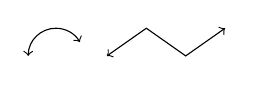
\begin{tikzpicture}
  \draw [<->] (0,0) arc [start angle=180, end angle=30, radius=10pt];
  \draw [<->] (1,0) -- (1.5cm,10pt) -- (2cm,0pt) -- (2.5cm,10pt);
\end{tikzpicture}
\end{codeexample}

Karl has a more detailed look at the arrow that \tikzname\ puts at the end. It
looks like this when he zooms it: \tikz[baseline] \draw[->,line width=1pt]
(0pt,.5ex) -- ++(10pt,0pt);. The shape seems vaguely familiar and, indeed, this
is exactly the end of \TeX's standard arrow used in something like $f\colon A
\to B$.

Karl likes the arrow, especially since it is not ``as thick'' as the arrows
offered by many other packages. However, he expects that, sometimes, he might
need to use some other kinds of arrow. To do so, Karl can say |>=|\meta{kind of
end arrow tip}, where \meta{kind of end arrow tip} is a special arrow tip
specification. For example, if Karl says |>=Stealth|, then he tells \tikzname\
that he would like  ``stealth-fighter-like'' arrow tips:
\todosp{remaining instance of bug \#473}
%
\begin{codeexample}[preamble={\usetikzlibrary{arrows.meta}}]
\begin{tikzpicture}[>=Stealth]
  \draw [->] (0,0) arc [start angle=180, end angle=30, radius=10pt];
  \draw [<<-,very thick] (1,0) -- (1.5cm,10pt) -- (2cm,0pt) -- (2.5cm,10pt);
\end{tikzpicture}
\end{codeexample}

Karl wonders whether such a military name for the arrow type is really
necessary. He is not really mollified when his son tells him that Microsoft's
PowerPoint uses the same name. He decides to have his students discuss this at
some point.

In addition to |Stealth| there are several other predefined kinds of arrow tips
Karl can choose from, see Section~\ref{section-arrows}. Furthermore, he can
define arrows types himself, if he needs new ones.


\subsection{Scoping}

Karl saw already that there are numerous graphic options that affect how paths
are rendered. Often, he would like to apply certain options to a whole set of
graphic commands. For example, Karl might wish to draw three paths using a
|thick| pen, but would like everything else to be drawn ``normally''.

If Karl wishes to set a certain graphic option for the whole picture, he can
simply pass this option to the |\tikz| command or to the |{tikzpicture}|
environment (Gerda would pass the options to |\tikzpicture| and Hans passes
them to |\starttikzpicture|). However, if Karl wants to apply graphic options
to a local group, he put these commands inside a |{scope}| environment (Gerda
uses |\scope| and |\endscope|, Hans uses |\startscope| and |\stopscope|). This
environment takes graphic options as an optional argument and these options
apply to everything inside the scope, but not to anything outside.

Here is an example:
%
\begin{codeexample}[]
\begin{tikzpicture}[ultra thick]
  \draw (0,0) -- (0,1);
  \begin{scope}[thin]
    \draw (1,0) -- (1,1);
    \draw (2,0) -- (2,1);
  \end{scope}
  \draw (3,0) -- (3,1);
\end{tikzpicture}
\end{codeexample}

Scoping has another interesting effect: Any changes to the clipping area are
local to the scope. Thus, if you say |\clip| somewhere inside a scope, the
effect of the |\clip| command ends at the end of the scope. This is useful
since there is no other way of ``enlarging'' the clipping area.

Karl has also already seen that giving options to commands like |\draw| apply
only to that command. It turns out that the situation is slightly more complex.
First, options to a command like |\draw| are not really options to the command,
but they are ``path options'' and can be given anywhere on the path. So,
instead of |\draw[thin] (0,0) -- (1,0);| one can also write
|\draw (0,0) [thin] -- (1,0);| or |\draw (0,0) -- (1,0) [thin];|; all of these
have the same effect. This might seem strange since in the last case, it would
appear that the |thin| should take effect only ``after'' the line from $(0,0)$
to $(1,0)$ has been drawn. However, most graphic options only apply to the
whole path. Indeed, if you say both |thin| and |thick| on the same path, the
last option given will ``win''.

When reading the above, Karl notices that only ``most'' graphic options apply
to the whole path. Indeed, all transformation options do \emph{not} apply to
the whole path, but only to ``everything following them on the path''. We will
have a more detailed look at this in a moment. Nevertheless, all options given
during a path construction apply only to this path.


\subsection{Transformations}

When you specify a  coordinate like |(1cm,1cm)|, where is that coordinate
placed on the page? To determine the position, \tikzname, \TeX, and
\textsc{pdf} or PostScript all apply certain transformations to the given
coordinate in order to determine the final position on the page.

\tikzname\ provides numerous options that allow you to transform coordinates in
\tikzname's private coordinate system. For example, the |xshift| option allows
you to shift all subsequent points by a certain amount:

\begin{codeexample}[]
\tikz \draw (0,0) -- (0,0.5) [xshift=2pt] (0,0) -- (0,0.5);
\end{codeexample}

It is important to note that you can change transformation ``in the middle of a
path'', a feature that is not supported by \pdf\ or PostScript. The reason is
that \tikzname\ keeps track of its own transformation matrix.

Here is a more complicated example:
%
\begin{codeexample}[]

\begin{tikzpicture}[even odd rule,rounded corners=2pt,x=10pt,y=10pt]
  \filldraw[fill=yellow!80!black] (0,0)   rectangle (1,1)
        [xshift=5pt,yshift=5pt]   (0,0)   rectangle (1,1)
                    [rotate=30]   (-1,-1) rectangle (2,2);
\end{tikzpicture}
\end{codeexample}

The most useful transformations are |xshift| and |yshift| for shifting, |shift|
for shifting to a given point as in |shift={(1,0)}| or |shift={+(0,0)}| (the
braces are necessary so that \TeX\ does not mistake the comma for separating
options), |rotate| for rotating by a certain angle (there is also a
|rotate around| for rotating around a given point), |scale| for scaling by a
certain factor, |xscale| and |yscale| for scaling only in the $x$- or
$y$-direction (|xscale=-1| is a flip), and |xslant| and |yslant| for slanting.
If these transformation and those that I have not mentioned are not sufficient,
the |cm| option allows you to apply an arbitrary transformation matrix. Karl's
students, by the way, do not know what a transformation matrix is.


\subsection{Repeating Things: For-Loops}

Karl's next aim is to add little ticks on the axes at positions $-1$, $-1/2$,
$1/2$, and $1$. For this, it would be nice to use some kind of ``loop'',
especially since he wishes to do the same thing at each of these positions.
There are different packages for doing this. \LaTeX\ has its own internal
command for this, |pstricks| comes along with the powerful |\multido| command.
All of these can be used together with \tikzname, so if you are familiar with
them, feel free to use them. \tikzname\ introduces yet another command, called
|\foreach|, which I introduced since I could never remember the syntax of the
other packages. |\foreach| is defined in the package |pgffor| and can be used
independently of \tikzname, but \tikzname\ includes it automatically.

In its basic form, the |\foreach| command is easy to use:
%
\begin{codeexample}[]
\foreach \x in {1,2,3} {$x =\x$, }
\end{codeexample}

The general syntax is
|\foreach| \meta{variable}| in {|\meta{list of values}|} |\meta{commands}.
Inside the \meta{commands}, the \meta{variable} will be assigned to the
different values. If the \meta{commands} do not start with a brace, everything
up to the next semicolon is used as \meta{commands}.

For Karl and the ticks on the axes, he could use the following code:
%
\begin{codeexample}[]
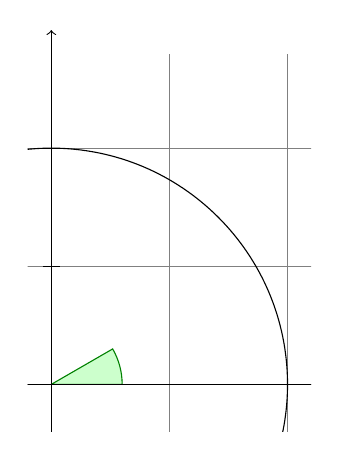
\begin{tikzpicture}[scale=3]
  \clip (-0.1,-0.2) rectangle (1.1,1.51);
  \draw[step=.5cm,gray,very thin] (-1.4,-1.4) grid (1.4,1.4);
  \filldraw[fill=green!20,draw=green!50!black] (0,0) -- (3mm,0mm)
      arc [start angle=0, end angle=30, radius=3mm] -- cycle;
  \draw[->] (-1.5,0) -- (1.5,0);
  \draw[->] (0,-1.5) -- (0,1.5);
  \draw (0,0) circle [radius=1cm];

  \foreach \x in {-1cm,-0.5cm,1cm}
    \draw (\x,-1pt) -- (\x,1pt);
  \foreach \y in {-1cm,-0.5cm,0.5cm,1cm}
    \draw (-1pt,\y) -- (1pt,\y);
\end{tikzpicture}
\end{codeexample}

As a matter of fact, there are many different ways of creating the ticks. For
example, Karl could have put the |\draw ...;| inside curly braces. He could
also have used, say,
%
\begin{codeexample}[code only]
\foreach \x in {-1,-0.5,1}
  \draw[xshift=\x cm] (0pt,-1pt) -- (0pt,1pt);
\end{codeexample}

Karl is curious what would happen in a more complicated situation where there
are, say, 20 ticks. It seems bothersome to explicitly mention all these numbers
in the set for |\foreach|. Indeed, it is possible to use |...| inside the
|\foreach| statement to iterate over a large number of values (which must,
however, be dimensionless real numbers) as in the following example:
%
\begin{codeexample}[]
\tikz \foreach \x in {1,...,10}
        \draw (\x,0) circle (0.4cm);
\end{codeexample}

If you provide \emph{two} numbers before the |...|, the |\foreach| statement
will use their difference for the stepping:
%
\begin{codeexample}[]
\tikz \foreach \x in {-1,-0.5,...,1}
       \draw (\x cm,-1pt) -- (\x cm,1pt);
\end{codeexample}

We can also nest loops to create interesting effects:
%
\begin{codeexample}[]
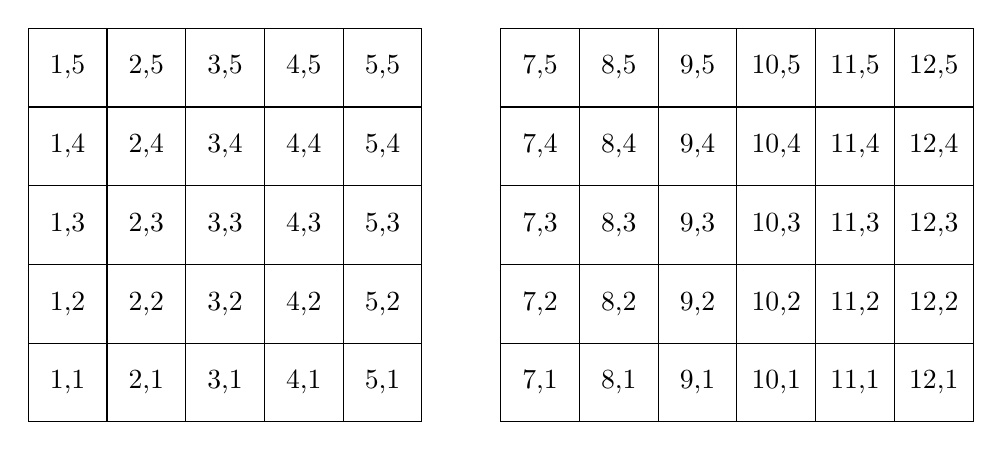
\begin{tikzpicture}
  \foreach \x in {1,2,...,5,7,8,...,12}
    \foreach \y in {1,...,5}
    {
      \draw (\x,\y) +(-.5,-.5) rectangle ++(.5,.5);
      \draw (\x,\y) node{\x,\y};
    }
\end{tikzpicture}
\end{codeexample}

The |\foreach| statement can do even trickier stuff, but the above gives the
idea.


\subsection{Adding Text}

Karl is, by now, quite satisfied with the picture. However, the most important
parts, namely the labels, are still missing!

\tikzname\ offers an easy-to-use and powerful system for adding text and, more
generally, complex shapes to a picture at specific positions. The basic idea is
the following: When \tikzname\ is constructing a path and encounters the
keyword |node| in the middle of a path, it reads a \emph{node specification}.
The keyword |node| is typically followed by some options and then some text
between curly braces. This text is put inside a normal \TeX\ box (if the node
specification directly follows a coordinate, which is usually the case,
\tikzname\ is able to perform some magic so that it is even possible to use
verbatim text inside the boxes) and then placed at the current position, that
is, at the last specified position (possibly shifted a bit, according to the
given options). However, all nodes are drawn only after the path has been
completely drawn/filled/shaded/clipped/whatever.
%
\begin{codeexample}[]
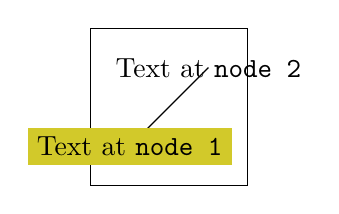
\begin{tikzpicture}
  \draw (0,0) rectangle (2,2);
  \draw (0.5,0.5) node [fill=yellow!80!black]
                       {Text at \verb!node 1!}
     -- (1.5,1.5) node {Text at \verb!node 2!};
\end{tikzpicture}
\end{codeexample}

Obviously, Karl would not only like to place nodes \emph{on} the last specified
position, but also to the left or the right of these positions. For this, every
node object that you put in your picture is equipped with several
\emph{anchors}. For example, the |north| anchor is in the middle at the upper
end of the shape, the |south| anchor is at the bottom and the |north east|
anchor is in the upper right corner. When you give the option |anchor=north|,
the text will be placed such that this northern anchor will lie on the current
position and the text is, thus, below the current position. Karl uses this to
draw the ticks as follows:
%
\begin{codeexample}[]
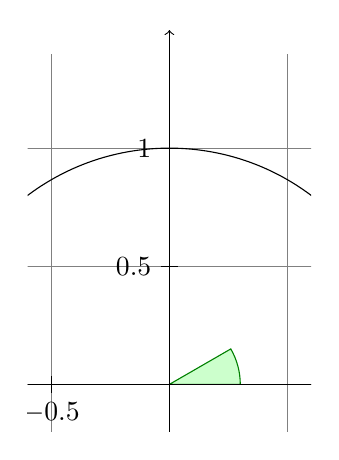
\begin{tikzpicture}[scale=3]
  \clip (-0.6,-0.2) rectangle (0.6,1.51);
  \draw[step=.5cm,help lines] (-1.4,-1.4) grid (1.4,1.4);
  \filldraw[fill=green!20,draw=green!50!black] (0,0) -- (3mm,0mm)
    arc [start angle=0, end angle=30, radius=3mm] -- cycle;
  \draw[->] (-1.5,0) -- (1.5,0);   \draw[->] (0,-1.5) -- (0,1.5);
  \draw (0,0) circle [radius=1cm];

  \foreach \x in {-1,-0.5,1}
    \draw (\x cm,1pt) -- (\x cm,-1pt) node[anchor=north] {$\x$};
  \foreach \y in {-1,-0.5,0.5,1}
    \draw (1pt,\y cm) -- (-1pt,\y cm) node[anchor=east] {$\y$};
\end{tikzpicture}
\end{codeexample}

This is quite nice, already. Using these anchors, Karl can now add most of the
other text elements. However, Karl thinks that, though ``correct'', it is quite
counter-intuitive that in order to place something \emph{below} a given point,
he has to use the \emph{north} anchor. For this reason, there is an option
called |below|, which does the same as |anchor=north|. Similarly, |above right|
does the same as |anchor=south west|. In addition, |below| takes an optional
dimension argument. If given, the shape will additionally be shifted downwards
by the given amount. So, |below=1pt| can be used to put a text label below some
point and, additionally shift it  1pt downwards.

Karl is not quite satisfied with the ticks. He would like to have $1/2$ or
$\frac{1}{2}$ shown instead of $0.5$, partly to show off the nice capabilities
of \TeX\ and \tikzname, partly because for positions like $1/3$ or $\pi$ it is
certainly very much preferable to have the ``mathematical'' tick there instead
of just the ``numeric'' tick. His students, on the other hand, prefer $0.5$
over $1/2$ since they are not too fond of fractions in general.

Karl now faces a problem: For the |\foreach| statement, the position |\x|
should still be given as |0.5| since \tikzname\ will not know where
|\frac{1}{2}| is supposed to be. On the other hand, the typeset text should
really be  |\frac{1}{2}|. To solve this problem, |\foreach| offers a special
syntax: Instead of having one variable |\x|, Karl can specify two (or even
more) variables separated by a slash as in |\x / \xtext|. Then, the elements in
the set over which |\foreach| iterates must also be of the form
\meta{first}|/|\meta{second}. In each iteration, |\x| will be set to
\meta{first} and |\xtext| will be set to \meta{second}. If no \meta{second} is
given, the \meta{first} will be used again. So, here is the new code for the
ticks:
%
\begin{codeexample}[]
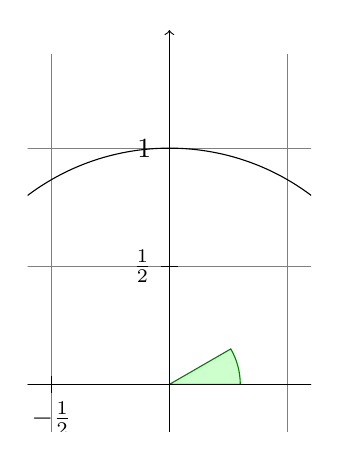
\begin{tikzpicture}[scale=3]
  \clip (-0.6,-0.2) rectangle (0.6,1.51);
  \draw[step=.5cm,help lines] (-1.4,-1.4) grid (1.4,1.4);
  \filldraw[fill=green!20,draw=green!50!black] (0,0) -- (3mm,0mm)
      arc [start angle=0, end angle=30, radius=3mm] -- cycle;
  \draw[->] (-1.5,0) -- (1.5,0); \draw[->] (0,-1.5) -- (0,1.5);
  \draw (0,0) circle [radius=1cm];

  \foreach \x/\xtext in {-1, -0.5/-\frac{1}{2}, 1}
    \draw (\x cm,1pt) -- (\x cm,-1pt) node[anchor=north] {$\xtext$};
  \foreach \y/\ytext in {-1, -0.5/-\frac{1}{2}, 0.5/\frac{1}{2}, 1}
    \draw (1pt,\y cm) -- (-1pt,\y cm) node[anchor=east] {$\ytext$};
\end{tikzpicture}
\end{codeexample}

Karl is quite pleased with the result, but his son points out that this is
still not perfectly satisfactory: The grid and the circle interfere with the
numbers and decrease their legibility. Karl is not very concerned by this (his
students do not even notice), but his son insists that there is an easy
solution: Karl can add the |[fill=white]| option to fill out the background of
the text shape with a white color.

The next thing Karl wants to do is to add the labels like $\sin \alpha$. For
this, he would like to place a label ``in the middle of the line''. To do so,
instead of specifying the label |node {$\sin\alpha$}|  directly after one of
the endpoints of the line (which would place the label at that endpoint), Karl
can give the label directly after the |--|, before the coordinate. By default,
this places the label in the middle of the line, but the |pos=| options can be
used to modify this. Also, options like |near start| and |near end| can be used
to modify this position:
%
\begin{codeexample}[preamble={\usetikzlibrary{intersections}}]
\begin{tikzpicture}[scale=3]
  \clip (-2,-0.2) rectangle (2,0.8);
  \draw[step=.5cm,gray,very thin] (-1.4,-1.4) grid (1.4,1.4);
  \filldraw[fill=green!20,draw=green!50!black] (0,0) -- (3mm,0mm)
    arc [start angle=0, end angle=30, radius=3mm] -- cycle;
  \draw[->] (-1.5,0) -- (1.5,0) coordinate (x axis);
  \draw[->] (0,-1.5) -- (0,1.5) coordinate (y axis);
  \draw (0,0) circle [radius=1cm];

  \draw[very thick,red]
    (30:1cm) -- node[left=1pt,fill=white] {$\sin \alpha$} (30:1cm |- x axis);
  \draw[very thick,blue]
    (30:1cm |- x axis) -- node[below=2pt,fill=white] {$\cos \alpha$} (0,0);
  \path [name path=upward line] (1,0) -- (1,1);
  \path [name path=sloped line] (0,0) -- (30:1.5cm);
  \draw [name intersections={of=upward line and sloped line, by=t}]
    [very thick,orange] (1,0) -- node [right=1pt,fill=white]
    {$\displaystyle \tan \alpha \color{black}=
      \frac{{\color{red}\sin \alpha}}{\color{blue}\cos \alpha}$} (t);

  \draw (0,0) -- (t);

  \foreach \x/\xtext in {-1, -0.5/-\frac{1}{2}, 1}
    \draw (\x cm,1pt) -- (\x cm,-1pt) node[anchor=north,fill=white] {$\xtext$};
  \foreach \y/\ytext in {-1, -0.5/-\frac{1}{2}, 0.5/\frac{1}{2}, 1}
    \draw (1pt,\y cm) -- (-1pt,\y cm) node[anchor=east,fill=white] {$\ytext$};
\end{tikzpicture}
\end{codeexample}

You can also position labels on curves and, by adding the |sloped| option, have
them rotated such that they match the line's slope. Here is an example:
%
\begin{codeexample}[]
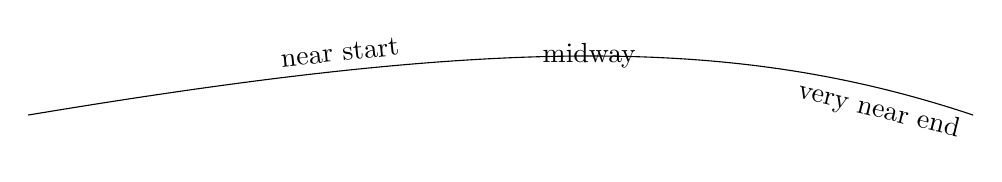
\begin{tikzpicture}
  \draw (0,0) .. controls (6,1) and (9,1) ..
    node[near start,sloped,above] {near start}
    node {midway}
    node[very near end,sloped,below] {very near end} (12,0);
\end{tikzpicture}
\end{codeexample}

It remains to draw the explanatory text at the right of the picture. The main
difficulty here lies in limiting the width of the text ``label'', which is
quite long, so that line breaking is used. Fortunately, Karl can use the option
|text width=6cm| to get the desired effect. So, here is the full code:
%
\begin{codeexample}[code only]
\begin{tikzpicture}
  [scale=3,line cap=round,
  % Styles
  axes/.style=,
  important line/.style={very thick},
  information text/.style={rounded corners,fill=red!10,inner sep=1ex}]

  % Colors
  \colorlet{anglecolor}{green!50!black}
  \colorlet{sincolor}{red}
  \colorlet{tancolor}{orange!80!black}
  \colorlet{coscolor}{blue}

  % The graphic
  \draw[help lines,step=0.5cm] (-1.4,-1.4) grid (1.4,1.4);

  \draw (0,0) circle [radius=1cm];

  \begin{scope}[axes]
    \draw[->] (-1.5,0) -- (1.5,0) node[right] {$x$} coordinate(x axis);
    \draw[->] (0,-1.5) -- (0,1.5) node[above] {$y$} coordinate(y axis);

    \foreach \x/\xtext in {-1, -.5/-\frac{1}{2}, 1}
      \draw[xshift=\x cm] (0pt,1pt) -- (0pt,-1pt) node[below,fill=white] {$\xtext$};

    \foreach \y/\ytext in {-1, -.5/-\frac{1}{2}, .5/\frac{1}{2}, 1}
      \draw[yshift=\y cm] (1pt,0pt) -- (-1pt,0pt) node[left,fill=white] {$\ytext$};
  \end{scope}

  \filldraw[fill=green!20,draw=anglecolor] (0,0) -- (3mm,0pt)
    arc [start angle=0, end angle=30, radius=3mm];
  \draw (15:2mm) node[anglecolor] {$\alpha$};

  \draw[important line,sincolor]
    (30:1cm) -- node[left=1pt,fill=white] {$\sin \alpha$} (30:1cm |- x axis);

  \draw[important line,coscolor]
    (30:1cm |- x axis) -- node[below=2pt,fill=white] {$\cos \alpha$} (0,0);

  \path [name path=upward line] (1,0) -- (1,1);
  \path [name path=sloped line] (0,0) -- (30:1.5cm);
  \draw [name intersections={of=upward line and sloped line, by=t}]
    [very thick,orange] (1,0) -- node [right=1pt,fill=white]
    {$\displaystyle \tan \alpha \color{black}=
      \frac{{\color{red}\sin \alpha}}{\color{blue}\cos \alpha}$} (t);

  \draw (0,0) -- (t);

  \draw[xshift=1.85cm]
    node[right,text width=6cm,information text]
    {
      The {\color{anglecolor} angle $\alpha$} is $30^\circ$ in the
      example ($\pi/6$ in radians). The {\color{sincolor}sine of
        $\alpha$}, which is the height of the red line, is
      \[
      {\color{sincolor} \sin \alpha} = 1/2.
      \]
      By the Theorem of Pythagoras ...
    };
\end{tikzpicture}
\end{codeexample}


\subsection{Pics: The Angle Revisited}

Karl expects that the code of certain parts of the picture he created might be
so useful that he might wish to reuse them in the future. A natural thing to do
is to create \TeX\ macros that store the code he wishes to reuse. However,
\tikzname\ offers another way that is integrated directly into its parser:
pics!

A ``pic'' is ``not quite a full picture'', hence the short name. The idea is
that a pic is simply some code that you can add to a picture at different
places using the |pic| command whose syntax is almost identical to the |node|
command. The main difference is that instead of specifying some text in curly
braces that should be shown, you specify the name of a predefined picture that
should be shown.

Defining new pics is easy enough, see Section~\ref{section-pics}, but right now
we just want to use one such predefined pic: the |angle| pic. As the name
suggests, it is a small drawing of an angle consisting of a little wedge and an
arc together with some text (Karl needs to load the |angles| library and the
|quotes| for the following examples). What makes this pic useful is the fact
that the size of the wedge will be computed automatically.

The |angle| pic draws an angle between the two lines $BA$ and $BC$, where $A$,
$B$, and $C$ are three coordinates. In our case, $B$ is the origin, $A$ is
somewhere on the $x$-axis and $C$ is somewhere on a line at $30^\circ$.
%
\begin{codeexample}[preamble={\usetikzlibrary{angles,quotes}}]
\begin{tikzpicture}[scale=3]
  \coordinate (A) at (1,0);
  \coordinate (B) at (0,0);
  \coordinate (C) at (30:1cm);

  \draw (A) -- (B) -- (C)
        pic [draw=green!50!black, fill=green!20, angle radius=9mm,
             "$\alpha$"] {angle = A--B--C};
\end{tikzpicture}
\end{codeexample}

Let us see, what is happening here. First we have specified three
\emph{coordinates} using the |\coordinate| command. It allows us to name a
specific coordinate in the picture. Then comes something that starts as a
normal |\draw|, but then comes the |pic| command. This command gets lots of
options and, in curly braces, comes the most important point: We specify that
we want to add an |angle| pic and this angle should be between the points we
named |A|, |B|, and |C| (we could use other names). Note that the text that we
want to be shown in the pic is specified in quotes inside the options of the
|pic|, not inside the curly braces.

To learn more about pics, please see Section~\ref{section-pics}.

% % Copyright 2006 by Tilo Tantau
%
% This file may be distributed and/or modified
%
% 1. under the LaTeX Project Public License and/or
% 2. under the GNU Free Documentation License.
%
% See the file doc/generic/pgf/licenses/LICENSE for more details.

% \section{Tutorial: A Petri-Net for Hagen}
\section{教程:给 Hagen 的 Petri 网}

\bohs

% In this second tutorial we explore the node mechanism of
% \tikzname\ and \pgfname.
在这第二个教程中,我们将探索 \tikzname\ 和 \pgfname\ 中的节点机制(node mechanism)。

% Hagen must give a talk tomorrow about his favorite formalism for
% distributed systems: Petri nets! Hagen used to give his talks using a
% blackboard and everyone seemed to be perfectly content with
% this. Unfortunately, his audience has been spoiled recently with fancy
% projector-based presentations and there seems to be a certain amount
% of peer pressure that his Petri nets should also be drawn using a
% graphic program. One of the professors at his institute recommends
% \tikzname\ for this and Hagen decides to give it a try.
Hagen 明天必须做一个报告,内容是他最爱的分布式系统的形式主义:Petri 网!
他过去都是用黑板做报告,每个人看上去都非常满意。
不幸的是,如今不少精致的报告用了投影仪,把他的听众惯坏了,所以 Hagen 感受到了来自同行的巨大压力,似乎他的 Petri 网也应该用图形程序绘制。
Hagen 的学院里有位教授给他推荐了 \tikzname,所以他决定试一试。

\eohs

% \subsection{Problem Statement}
\subsection{问题陈述}

\bohs

% For his talk, Hagen wishes to create a graphic that demonstrates how a
% net with place capacities can be simulated by a net without
% capacities. The graphic should look like this, ideally:


\eohs

\begin{quote}
\begin{tikzpicture}
  [node distance=1.3cm,>=stealth',bend angle=45,auto,
   place/.style={circle,thick,draw=blue!75,fill=blue!20,minimum size=6mm},
   red place/.style={place,draw=red!75,fill=red!20},
   transition/.style={rectangle,thick,draw=black!75,fill=black!20,minimum size=4mm},
   every label/.style={red},on grid]

  \begin{scope}
    % First net
    \node [place,tokens=1] (w1)                                    {};
    \node [place] (c1) [below=of w1]                      {};
    \node [place] (s)  [below=of c1,label=above:$s\le 3$] {};
    \node [place] (c2) [below=of s]                       {};
    \node [place,tokens=1] (w2) [below=of c2]                      {};

    \node [transition] (e1) [left=of c1] {}
      edge [pre,bend left]                  (w1)
      edge [post,bend right]                (s)
      edge [post]                           (c1);

    \node [transition] (e2) [left=of c2] {}
      edge [pre,bend right]                 (w2)
      edge [post,bend left]                 (s)
      edge [post]                           (c2);

    \node [transition] (l1) [right=of c1] {}
      edge [pre]                            (c1)
      edge [pre,bend left]                  (s)
      edge [post,bend right] node[swap] {2} (w1);

    \node [transition] (l2) [right=of c2] {}
      edge [pre]                            (c2)
      edge [pre,bend right]                 (s)
      edge [post,bend left]  node {2}       (w2);
  \end{scope}

  \begin{scope}[xshift=6cm]
    % Second net
    \node [place,tokens=1]
                      (w1')                                                {};
    \node [place]     (c1') [below=of w1']                                 {};
    \node [red place] (s1') [below=of c1',xshift=-5mm,label=left:$s$]      {};
    \node [red place,tokens=3]
                      (s2') [below=of c1',xshift=5mm,label=right:$\bar s$] {};
    \node [place]     (c2') [below=of s1',xshift=5mm]                      {};
    \node [place,tokens=1]
                      (w2') [below=of c2']                                 {};

    \node [transition] (e1') [left=of c1'] {}
      edge [pre,bend left]                  (w1')
      edge [post]                           (s1')
      edge [pre]                            (s2')
      edge [post]                           (c1');

    \node [transition] (e2') [left=of c2'] {}
      edge [pre,bend right]                 (w2')
      edge [post]                           (s1')
      edge [pre]                            (s2')
      edge [post]                           (c2');

    \node [transition] (l1') [right=of c1'] {}
      edge [pre]                            (c1')
      edge [pre]                            (s1')
      edge [post]                           (s2')
      edge [post,bend right] node[swap] {2} (w1');

    \node [transition] (l2') [right=of c2'] {}
      edge [pre]                            (c2')
      edge [pre]                            (s1')
      edge [post]                           (s2')
      edge [post,bend left]  node {2}       (w2');
  \end{scope}

  \begin{scope}[on background layer]
    \node (r1) [fill=black!10,rounded corners,fit=(w1)(w2)(e1)(e2)(l1)(l2)] {};
    \node (r2) [fill=black!10,rounded corners,fit=(w1')(w2')(e1')(e2')(l1')(l2')] {};
  \end{scope}

  \draw [shorten >=1mm,-to,thick,decorate,decoration={snake,amplitude=.4mm,segment
      length=2mm,pre=moveto,pre length=1mm,post length=2mm}]
    (r1) -- (r2)
    node [above=1mm,midway,text width=3cm,align=center]
      {replacement of the \textcolor{red}{capacity} by \textcolor{red}{two places}};

\end{tikzpicture}
\end{quote}


\subsection{Setting up the Environment}

For the picture Hagen will need to load the \tikzname\ package as did
Karl in the previous tutorial. However, Hagen will also need to load
some additional  \emph{library packages} that Karl did not need. These
library packages contain additional definitions like extra arrow tips
that are typically not needed in a picture and that need to be
loaded explicitly.

Hagen will need to load several libraries: The |arrows| library for the
special arrow tip used in the graphic, the |decoration.pathmorphing|
library for the ``snaking line'' in the middle, the |backgrounds|
library for the two rectangular areas that are behind the two main
parts of the picture, the |fit| library to easily compute the sizes of
these rectangles, and the |positioning| library for placing nodes
relative to other nodes.


\subsubsection{Setting up the Environment in \LaTeX}

When using \LaTeX\ use:

\begin{codeexample}[code only]
\documentclass{article} % say

\usepackage{tikz}
\usetikzlibrary{arrows,decorations.pathmorphing,backgrounds,positioning,fit,petri}

\begin{document}
\begin{tikzpicture}
  \draw (0,0) -- (1,1);
\end{tikzpicture}
\end{document}
\end{codeexample}


\subsubsection{Setting up the Environment in Plain \TeX}

When using plain \TeX\ use:

\begin{codeexample}[code only]
%% Plain TeX file
\input tikz.tex
\usetikzlibrary{arrows,decorations.pathmorphing,backgrounds,positioning,fit,petri}
\baselineskip=12pt
\hsize=6.3truein
\vsize=8.7truein
\tikzpicture
  \draw (0,0) -- (1,1);
\endtikzpicture
\bye
\end{codeexample}


\subsubsection{Setting up the Environment in Con\TeX t}

When using Con\TeX, use:
\begin{codeexample}[code only]
%% ConTeXt file
\usemodule[tikz]
\usetikzlibrary[arrows,decorations.pathmorphing,backgrounds,positioning,fit,petri]

\starttext
  \starttikzpicture
    \draw (0,0) -- (1,1);
  \stoptikzpicture
\stoptext
\end{codeexample}



\subsection{Introduction to Nodes}

In principle, we already know how to create the graphics that Hagen
desires (except perhaps for the snaked line, we will come to that): We
start with big light gray rectangle and then add lots of circles and
small rectangle, plus some arrows.

However, this approach has numerous disadvantages: First, it is hard
to change anything at a later stage. For example, if we decide to add
more places to the Petri nets (the circles are called places in Petri
net theory), all of the coordinates change and we need to recalculate
everything. Second, it is hard to read the code for the Petri net as it is just a long and complicated list of coordinates and drawing
commands -- the underlying structure of the Petri net is lost.

Fortunately, \tikzname\ offers a powerful mechanism for avoiding the
above problems: nodes. We already came across nodes in the previous
tutorial, where we used them to add labels to Karl's graphic. In the
present tutorial we will see that nodes are much more powerful.

A node is a small part of a picture. When a node is created, you
provide a position where the node should be drawn and a
\emph{shape}. A node of shape |circle| will be drawn as a circle, a
node of shape |rectangle| as a rectangle, and so on. A node may also
contain some text, which is why Karl used nodes to show text. Finally,
a node can get a \emph{name} for later reference.

In Hagen's picture we will use nodes for the places and for the
transitions of the Petri net (the places are the circles, the
transitions are the rectangles). Let us start with the upper half of
the left Petri net. In this upper half we have three places and two
transitions. Instead of drawing three circles and two rectangles, we
use three nodes of shape |circle| and two nodes of shape
|rectangle|.

\begin{codeexample}[]
\begin{tikzpicture}
  \path ( 0,2) node [shape=circle,draw] {}
        ( 0,1) node [shape=circle,draw] {}
        ( 0,0) node [shape=circle,draw] {}
        ( 1,1) node [shape=rectangle,draw] {}
        (-1,1) node [shape=rectangle,draw] {};
\end{tikzpicture}
\end{codeexample}

Hagen notes that this does not quite look like the final picture, but
it seems like a good first step.

Let us have a more detailed look at the code. The whole picture
consists of a single path. Ignoring the |node| operations, there is not
much going on in this path: It is just a sequence of coordinates with
nothing ``happening'' between them. Indeed, even if something were to
happen like a line-to or a curve-to, the |\path| command would not
``do'' anything with the resulting path. So, all the magic must be in
the |node| commands.

In the previous tutorial we learned that a |node| will add a piece of
text at the last coordinate. Thus, each of the five nodes is added at
a different position. In the above code, this text is empty
(because of the empty |{}|). So, why do we see anything at all? The
answer is the |draw| option for the |node| operation: It causes the
``shape around the text'' to be drawn.

So, the code |(0,2) node [shape=circle,draw] {}| means the following:
``In the main path, add a move-to to the coordinate |(0,2)|. Then,
temporarily suspend the construction of the main path while the node
is built. This node will be a |circle| around an empty text. This
circle is to be |draw|n, but not filled or otherwise used. Once this
whole node is constructed, it is saved until after the
main path is finished. Then, it is drawn.'' The following
|(0,1) node [shape=circle,draw] {}| then has the following effect:
``Continue the main path with a move-to to |(0,1)|. Then construct a
node at this position also. This node is also shown after the main
path is finished.'' And so on.



\subsection{Placing Nodes Using the At Syntax}

Hagen now understands how the |node| operation adds nodes to the path,
but it seems a bit silly to create a path using the |\path| operation,
consisting of numerous superfluous move-to operations, only to place
nodes. He is pleased to learn that there are ways to add nodes in a
more sensible manner.

First, the |node| operation allows one to add
|at (|\meta{coordinate}|)| in order to directly specify where the node
should be placed, sidestepping the rule that nodes are placed on the
last coordinate. Hagen can then write the following:

\begin{codeexample}[]
\begin{tikzpicture}
  \path node at ( 0,2) [shape=circle,draw] {}
        node at ( 0,1) [shape=circle,draw] {}
        node at ( 0,0) [shape=circle,draw] {}
        node at ( 1,1) [shape=rectangle,draw] {}
        node at (-1,1) [shape=rectangle,draw] {};
\end{tikzpicture}
\end{codeexample}

Now Hagen is still left with a single empty path, but at least the
path no longer contains strange move-tos. It turns out that this can
be improved further: The |\node| command is an abbreviation for
|\path node|, which allows Hagen to write:

\begin{codeexample}[]
\begin{tikzpicture}
  \node at ( 0,2) [circle,draw] {};
  \node at ( 0,1) [circle,draw] {};
  \node at ( 0,0) [circle,draw] {};
  \node at ( 1,1) [rectangle,draw] {};
  \node at (-1,1) [rectangle,draw] {};
\end{tikzpicture}
\end{codeexample}

Hagen likes this syntax much better than the previous one. Note that
Hagen has also omitted the |shape=| since, like |color=|, \tikzname\
allows you to omit the |shape=| if there is no confusion.



\subsection{Using Styles}

Feeling adventurous, Hagen tries to make the nodes look nicer. In the
final picture, the circles and rectangle should be filled with
different colors, resulting in the following code:

\begin{codeexample}[]
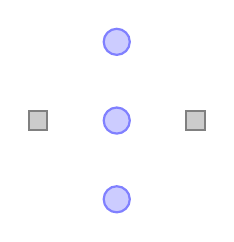
\begin{tikzpicture}[thick]
  \node at ( 0,2) [circle,draw=blue!50,fill=blue!20] {};
  \node at ( 0,1) [circle,draw=blue!50,fill=blue!20] {};
  \node at ( 0,0) [circle,draw=blue!50,fill=blue!20] {};
  \node at ( 1,1) [rectangle,draw=black!50,fill=black!20] {};
  \node at (-1,1) [rectangle,draw=black!50,fill=black!20] {};
\end{tikzpicture}
\end{codeexample}

While this looks nicer in the picture, the code starts to get a bit
ugly. Ideally, we would like our code to transport the message ``there
are three places and two transitions'' and not so much which
filling colors should be used.

To solve this problem, Hagen uses styles. He defines a style for
places and another style for transitions:

\begin{codeexample}[]
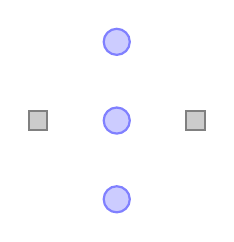
\begin{tikzpicture}
  [place/.style={circle,draw=blue!50,fill=blue!20,thick},
   transition/.style={rectangle,draw=black!50,fill=black!20,thick}]
  \node at ( 0,2) [place] {};
  \node at ( 0,1) [place] {};
  \node at ( 0,0) [place] {};
  \node at ( 1,1) [transition] {};
  \node at (-1,1) [transition] {};
\end{tikzpicture}
\end{codeexample}


\subsection{Node Size}

Before Hagen starts naming and connecting the nodes, let us first
make sure that the nodes get their final appearance. They are still
too small. Indeed, Hagen wonders why they have any size at all, after
all, the text is empty. The reason is that \tikzname\ automatically
adds some space around the text. The amount is set using the option
|inner sep|. So, to increase the size of the nodes, Hagen could write:

\begin{codeexample}[]
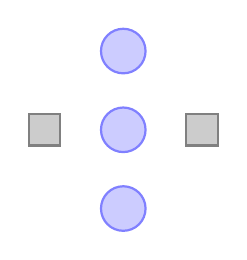
\begin{tikzpicture}
  [inner sep=2mm,
   place/.style={circle,draw=blue!50,fill=blue!20,thick},
   transition/.style={rectangle,draw=black!50,fill=black!20,thick}]
  \node at ( 0,2) [place] {};
  \node at ( 0,1) [place] {};
  \node at ( 0,0) [place] {};
  \node at ( 1,1) [transition] {};
  \node at (-1,1) [transition] {};
\end{tikzpicture}
\end{codeexample}

However, this is not really the best way to achieve the desired
effect. It is much better to use the |minimum size| option
instead. This option allows Hagen to specify a minimum size that the
node should have. If the node actually needs to be bigger because of
a longer text, it will be larger, but if the text is empty, then the
node will have |minimum size|. This option is also useful to ensure
that several nodes containing different amounts of text have the same
size. The options |minimum height| and |minimum width| allow you to
specify the minimum height and width independently.

So, what Hagen needs to do is to provide |minimum size| for the
nodes. To be on the safe side, he also sets |inner sep=0pt|. This
ensures that the nodes will really have size |minimum size| and not,
for very small minimum sizes, the minimal size necessary to encompass
the automatically added space.

\begin{codeexample}[]
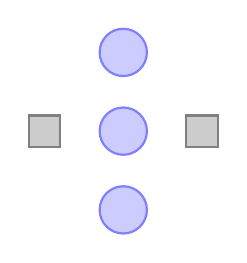
\begin{tikzpicture}
  [place/.style={circle,draw=blue!50,fill=blue!20,thick,
                 inner sep=0pt,minimum size=6mm},
   transition/.style={rectangle,draw=black!50,fill=black!20,thick,
                      inner sep=0pt,minimum size=4mm}]
  \node at ( 0,2) [place] {};
  \node at ( 0,1) [place] {};
  \node at ( 0,0) [place] {};
  \node at ( 1,1) [transition] {};
  \node at (-1,1) [transition] {};
\end{tikzpicture}
\end{codeexample}




\subsection{Naming Nodes}

Hagen's next aim is to connect the nodes using arrows. This seems like
a tricky business since the arrows should not start in the middle of
the nodes, but somewhere on the border and Hagen would very much like
to avoid computing these positions by hand.

Fortunately, \pgfname\ will perform all the necessary calculations for
him. However, he first has to assign names to the nodes so that he can
reference them later on.

There are two ways to name a node. The first is to use the |name=|
option. The second method is to write the desired name in parentheses
after the |node| operation. Hagen thinks that this second method seems
strange, but he will soon change his opinion.

{
\tikzset{place/.style={circle,draw=blue!50,fill=blue!20,thick,
                   inner sep=0pt,minimum size=6mm},
transition/.style={rectangle,draw=black!50,fill=black!20,thick,
                        inner sep=0pt,minimum size=4mm}}
\begin{codeexample}[]
% ... set up styles
\begin{tikzpicture}
  \node (waiting 1)  at ( 0,2)     [place] {};
  \node (critical 1) at ( 0,1)     [place] {};
  \node (semaphore)  at ( 0,0)     [place] {};
  \node (leave critical) at ( 1,1) [transition] {};
  \node (enter critical) at (-1,1) [transition] {};
\end{tikzpicture}
\end{codeexample}
}

Hagen is pleased to note that the names help in understanding the
code. Names for nodes can be pretty arbitrary, but they should not
contain commas, periods, parentheses, colons, and some other special
characters. However, they can contain underscores and hyphens.

The syntax for the |node| operation is quite liberal with respect to
the order in which node names, the |at| specifier, and the options
must come. Indeed, you can even have multiple option blocks between
the |node| and the text in curly braces, they accumulate. You can
rearrange them arbitrarily and perhaps the following might be preferable:

{
\tikzset{place/.style={circle,draw=blue!50,fill=blue!20,thick,
                   inner sep=0pt,minimum size=6mm},
transition/.style={rectangle,draw=black!50,fill=black!20,thick,
                        inner sep=0pt,minimum size=4mm}}
\begin{codeexample}[]
\begin{tikzpicture}
  \node[place]      (waiting 1)      at ( 0,2) {};
  \node[place]      (critical 1)     at ( 0,1) {};
  \node[place]      (semaphore)      at ( 0,0) {};
  \node[transition] (leave critical) at ( 1,1) {};
  \node[transition] (enter critical) at (-1,1) {};
\end{tikzpicture}
\end{codeexample}
}



\subsection{Placing Nodes Using Relative Placement}

Although Hagen still wishes to connect the nodes, he first wishes to
address another problem again: The placement of the nodes. Although he
likes the |at| syntax, in this particular case he would prefer placing
the nodes ``relative to each other.'' So, Hagen would like to say that
the |critical 1| node should be below the |waiting 1| node, wherever
the |waiting 1| node might be. There are different ways of achieving
this, but the nicest one in Hagen's case is the |below| option:

{
\tikzset{place/.style={circle,draw=blue!50,fill=blue!20,thick,
                   inner sep=0pt,minimum size=6mm},
transition/.style={rectangle,draw=black!50,fill=black!20,thick,
                        inner sep=0pt,minimum size=4mm}}
\begin{codeexample}[]
\begin{tikzpicture}
  \node[place]      (waiting)                            {};
  \node[place]      (critical)       [below=of waiting]  {};
  \node[place]      (semaphore)      [below=of critical] {};
  \node[transition] (leave critical) [right=of critical] {};
  \node[transition] (enter critical) [left=of critical]  {};
\end{tikzpicture}
\end{codeexample}
}

With the |positioning| library loaded, when an option like |below|
is followed by |of|, then the position of the node is shifted in
such a manner that it is placed at the distance |node distance| in the
specified direction of the given direction. The |node distance| is
either the distance between the centers of the nodes (when the
|on grid| option is set to true) or the distance between the borders
(when the |on grid| option is set to false, which is the default).

Even though the above code has the same effect as the earlier code, Hagen
can pass it to his colleagues who will be able to just read and
understand it, perhaps without even having to see the picture.



\subsection{Adding Labels Next to Nodes}

Before we have a look at how Hagen can connect the nodes, let us add
the capacity ``$s \le 3$'' to the bottom node. For this, two
approaches are possible:
\begin{enumerate}
\item Hagen can just add a new node above the |north| anchor of the
  |semaphore| node.
{
\tikzset{place/.style={circle,draw=blue!50,fill=blue!20,thick,
                   inner sep=0pt,minimum size=6mm},
transition/.style={rectangle,draw=black!50,fill=black!20,thick,
                        inner sep=0pt,minimum size=4mm}}
\begin{codeexample}[]
\begin{tikzpicture}
  \node[place]      (waiting)                            {};
  \node[place]      (critical)       [below=of waiting]  {};
  \node[place]      (semaphore)      [below=of critical] {};
  \node[transition] (leave critical) [right=of critical] {};
  \node[transition] (enter critical) [left=of critical]  {};

  \node [red,above] at (semaphore.north) {$s\le 3$};
\end{tikzpicture}
\end{codeexample}
}
This is a general approach that will ``always work.''

\item Hagen can use the special |label| option. This option is given
  to a |node| and it causes \emph{another} node to be added next to
  the node where the option is given. Here is the idea: When we
  construct the |semaphore| node, we wish to indicate that we want
  another node with the capacity above it. For this, we use the option
  |label=above:$s\le 3$|. This option is interpreted as follows: We
  want a node above the |semaphore| node and this node should read
  ``$s \le 3$.'' Instead of |above| we could also use things like
  |below left| before the colon or a number like |60|.
{
\tikzset{place/.style={circle,draw=blue!50,fill=blue!20,thick,
                   inner sep=0pt,minimum size=6mm},
transition/.style={rectangle,draw=black!50,fill=black!20,thick,
                        inner sep=0pt,minimum size=4mm}}
\begin{codeexample}[]
\begin{tikzpicture}
  \node[place]      (waiting)                            {};
  \node[place]      (critical)       [below=of waiting]  {};
  \node[place]      (semaphore)      [below=of critical,
                                      label=above:$s\le3$] {};
  \node[transition] (leave critical) [right=of critical] {};
  \node[transition] (enter critical) [left=of critical]  {};
\end{tikzpicture}
\end{codeexample}
}
  It is also possible to give multiple |label| options, this causes
  multiple labels to be drawn.
\begin{codeexample}[]
\tikz
  \node [circle,draw,label=60:$60^\circ$,label=below:$-90^\circ$] {my circle};
\end{codeexample}
  Hagen is not fully satisfied with the |label| option since the label
  is not red. To achieve this, he has two options: First, he can
  redefine the |every label| style. Second, he can add options to the
  label's node. These options are given following the |label=|, so he
  would write |label=[red]above:$s\le3$|. However, this does not quite
  work since \TeX\ thinks that the |]| closes the whole option list of
  the |semaphore| node. So, Hagen has to add braces and writes
  |label={[red]above:$s\le3$}|. Since this looks a bit ugly, Hagen
  decides to redefine the |every label| style.
{
\tikzset{place/.style={circle,draw=blue!50,fill=blue!20,thick,
                   inner sep=0pt,minimum size=6mm},
transition/.style={rectangle,draw=black!50,fill=black!20,thick,
                        inner sep=0pt,minimum size=4mm}}
\begin{codeexample}[]
\begin{tikzpicture}[every label/.style={red}]
  \node[place]      (waiting)                            {};
  \node[place]      (critical)       [below=of waiting]  {};
  \node[place]      (semaphore)      [below=of critical,
                                      label=above:$s\le3$] {};
  \node[transition] (leave critical) [right=of critical] {};
  \node[transition] (enter critical) [left=of critical]  {};
\end{tikzpicture}
\end{codeexample}
}
\end{enumerate}



\subsection{Connecting Nodes}

It is now high time to connect the nodes. Let us start with something
simple, namely with the straight line from |enter critical| to
|critical|. We want this line to start at the right side of
|enter critical| and to end at the left side of |critical|. For
this, we can use the \emph{anchors} of the nodes. Every node defines a
whole bunch of anchors that lie on its border or inside it. For
example, the |center| anchor is at the center of the node, the |west|
anchor is on the left of the node, and so on. To access the coordinate
of a node, we use a coordinate that contains the node's name followed
by a dot, followed by the anchor's name:

{
\tikzset{place/.style={circle,draw=blue!50,fill=blue!20,thick,
                   inner sep=0pt,minimum size=6mm},
transition/.style={rectangle,draw=black!50,fill=black!20,thick,
                        inner sep=0pt,minimum size=4mm}}
\begin{codeexample}[]
\begin{tikzpicture}
  \node[place]      (waiting)                            {};
  \node[place]      (critical)       [below=of waiting]  {};
  \node[place]      (semaphore)      [below=of critical] {};
  \node[transition] (leave critical) [right=of critical] {};
  \node[transition] (enter critical) [left=of critical]  {};
  \draw [->] (critical.west) -- (enter critical.east);
\end{tikzpicture}
\end{codeexample}
}

Next, let us tackle the curve from |waiting| to |enter critical|. This
can be specified using curves and controls:

{
\tikzset{place/.style={circle,draw=blue!50,fill=blue!20,thick,
                   inner sep=0pt,minimum size=6mm},
transition/.style={rectangle,draw=black!50,fill=black!20,thick,
                        inner sep=0pt,minimum size=4mm}}
\begin{codeexample}[]
\begin{tikzpicture}
  \node[place]      (waiting)                            {};
  \node[place]      (critical)       [below=of waiting]  {};
  \node[place]      (semaphore)      [below=of critical] {};
  \node[transition] (leave critical) [right=of critical] {};
  \node[transition] (enter critical) [left=of critical]  {};
  \draw [->] (enter critical.east) -- (critical.west);
  \draw [->] (waiting.west) .. controls +(left:5mm) and +(up:5mm)
                            .. (enter critical.north);
\end{tikzpicture}
\end{codeexample}
}

Hagen sees how he can now add all his edges, but the whole process
seems a but awkward and not very flexible. Again, the code seems to
obscure the structure of the graphic rather than showing it.

So, let us start improving the code for the edges. First, Hagen can
leave out the anchors:

{
\tikzset{place/.style={circle,draw=blue!50,fill=blue!20,thick,
                   inner sep=0pt,minimum size=6mm},
transition/.style={rectangle,draw=black!50,fill=black!20,thick,
                        inner sep=0pt,minimum size=4mm}}
\begin{codeexample}[]
\begin{tikzpicture}
  \node[place]      (waiting)                            {};
  \node[place]      (critical)       [below=of waiting]  {};
  \node[place]      (semaphore)      [below=of critical] {};
  \node[transition] (leave critical) [right=of critical] {};
  \node[transition] (enter critical) [left=of critical]  {};
  \draw [->] (enter critical) -- (critical);
  \draw [->] (waiting) .. controls +(left:8mm) and +(up:8mm)
                       .. (enter critical);
\end{tikzpicture}
\end{codeexample}
}

Hagen is a bit surprised that this works. After all, how did
\tikzname\ know that the line from |enter critical| to |critical|
should actually start on the borders? Whenever \tikzname\ encounters a
whole node name as a ``coordinate,'' it tries to ``be smart'' about
the anchor that it should choose for this node. Depending on what
happens next, \tikzname\ will choose an anchor that lies on the border
of the node on a line to the next coordinate or control point. The
exact rules are a bit complex, but the chosen point will usually be
correct -- and when it is not, Hagen can still specify the desired
anchor by hand.

Hagen would now like to simplify the curve operation somehow. It turns
out that this can be accomplished using a special path operation: the
|to| operation. This operation takes many options (you can even define
new ones yourself). One pair of options is useful for Hagen: The pair
|in| and |out|. These options take angles at which a curve should
leave or reach the start or target coordinates. Without these options,
a straight line is drawn:

{
\tikzset{place/.style={circle,draw=blue!50,fill=blue!20,thick,
                   inner sep=0pt,minimum size=6mm},
transition/.style={rectangle,draw=black!50,fill=black!20,thick,
                        inner sep=0pt,minimum size=4mm}}
\begin{codeexample}[]
\begin{tikzpicture}
  \node[place]      (waiting)                            {};
  \node[place]      (critical)       [below=of waiting]  {};
  \node[place]      (semaphore)      [below=of critical] {};
  \node[transition] (leave critical) [right=of critical] {};
  \node[transition] (enter critical) [left=of critical]  {};
  \draw [->] (enter critical) to                 (critical);
  \draw [->] (waiting)        to [out=180,in=90] (enter critical);
\end{tikzpicture}
\end{codeexample}
}

There is another option for the |to| operation, that is even better
suited to Hagen's problem: The |bend right| option. This option also
takes an angle, but this angle only specifies the angle by which the
curve is bent to the right:

{
\tikzset{place/.style={circle,draw=blue!50,fill=blue!20,thick,
                   inner sep=0pt,minimum size=6mm},
transition/.style={rectangle,draw=black!50,fill=black!20,thick,
                        inner sep=0pt,minimum size=4mm}}
\begin{codeexample}[]
\begin{tikzpicture}
  \node[place]      (waiting)                            {};
  \node[place]      (critical)       [below=of waiting]  {};
  \node[place]      (semaphore)      [below=of critical] {};
  \node[transition] (leave critical) [right=of critical] {};
  \node[transition] (enter critical) [left=of critical]  {};
  \draw [->] (enter critical) to                 (critical);
  \draw [->] (waiting)        to [bend right=45] (enter critical);
  \draw [->] (enter critical) to [bend right=45] (semaphore);
\end{tikzpicture}
\end{codeexample}
}

It is now time for Hagen to learn about yet another way of specifying
edges: Using the |edge| path operation. This operation is very similar
to the |to| operation, but there is one important difference: Like a
node the edge generated by the |edge| operation is not part of the
main path, but is added only later. This may not seem very important,
but it has some nice consequences. For example, every edge can have
its own arrow tips and its own color and so on and, still, all the
edges can be given on the same path. This allows Hagen to write the
following:


{
\tikzset{place/.style={circle,draw=blue!50,fill=blue!20,thick,
                   inner sep=0pt,minimum size=6mm},
transition/.style={rectangle,draw=black!50,fill=black!20,thick,
                        inner sep=0pt,minimum size=4mm}}
\begin{codeexample}[]
\begin{tikzpicture}
  \node[place]      (waiting)                            {};
  \node[place]      (critical)       [below=of waiting]  {};
  \node[place]      (semaphore)      [below=of critical] {};
  \node[transition] (leave critical) [right=of critical] {};
  \node[transition] (enter critical) [left=of critical]  {}
    edge [->]               (critical)
    edge [<-,bend left=45]  (waiting)
    edge [->,bend right=45] (semaphore);
\end{tikzpicture}
\end{codeexample}
}

Each |edge| caused a new path to be constructed, consisting of a |to|
between the node |enter critical| and the node following the |edge|
command.

The finishing touch is to introduce two styles |pre| and |post| and to
use the |bend angle=45| option to set the bend angle once and for all:

{
\tikzset{place/.style={circle,draw=blue!50,fill=blue!20,thick,
                   inner sep=0pt,minimum size=6mm},
transition/.style={rectangle,draw=black!50,fill=black!20,thick,
                        inner sep=0pt,minimum size=4mm}}
\begin{codeexample}[]
% Styles place and transition as before
\begin{tikzpicture}
  [bend angle=45,
   pre/.style={<-,shorten <=1pt,>=stealth',semithick},
   post/.style={->,shorten >=1pt,>=stealth',semithick}]

  \node[place]      (waiting)                            {};
  \node[place]      (critical)       [below=of waiting]  {};
  \node[place]      (semaphore)      [below=of critical] {};

  \node[transition] (leave critical) [right=of critical] {}
    edge [pre]             (critical)
    edge [post,bend right] (waiting)
    edge [pre, bend left]  (semaphore);
  \node[transition] (enter critical) [left=of critical]  {}
    edge [post]            (critical)
    edge [pre, bend left]  (waiting)
    edge [post,bend right] (semaphore);
\end{tikzpicture}
\end{codeexample}
}




\subsection{Adding Labels Next to Lines}

The next thing that Hagen needs to add is the ``$2$'' at the arcs. For
this Hagen can use \tikzname's automatic node placement: By adding the
option |auto|, \tikzname\ will position nodes on curves and lines in
such a way that they are not on the curve but next to it. Adding
|swap| will mirror the label with respect to the line. Here is a
general example:

{
\begin{codeexample}[]
\begin{tikzpicture}[auto,bend right]
  \node (a) at (0:1) {$0^\circ$};
  \node (b) at (120:1) {$120^\circ$};
  \node (c) at (240:1) {$240^\circ$};

  \draw (a) to node {1} node [swap] {1'} (b)
        (b) to node {2} node [swap] {2'} (c)
        (c) to node {3} node [swap] {3'} (a);
\end{tikzpicture}
\end{codeexample}
}

What is happening here? The nodes are given somehow inside the |to|
operation! When this is done, the node is placed on the middle of the
curve or line created by the |to| operation. The |auto| option then
causes the node to be moved in such a way that it does not lie on the
curve, but next to it. In the example we provide even two nodes on
each |to| operation.

For Hagen that |auto| option is not really necessary since the two
``2'' labels could also easily be placed ``by hand.'' However, in a
complicated plot with numerous edges automatic placement can be a
blessing.

{
\tikzset{place/.style={circle,draw=blue!50,fill=blue!20,thick,
                   inner sep=0pt,minimum size=6mm},
transition/.style={rectangle,draw=black!50,fill=black!20,thick,
                        inner sep=0pt,minimum size=4mm},
pre/.style={<-,shorten <=1pt,>=stealth',semithick},
post/.style={->,shorten >=1pt,>=stealth',semithick}}
\begin{codeexample}[]
% Styles as before
\begin{tikzpicture}[bend angle=45]
  \node[place]      (waiting)                            {};
  \node[place]      (critical)       [below=of waiting]  {};
  \node[place]      (semaphore)      [below=of critical] {};

  \node[transition] (leave critical) [right=of critical] {}
    edge [pre]                                 (critical)
    edge [post,bend right] node[auto,swap] {2} (waiting)
    edge [pre, bend left]                      (semaphore);
  \node[transition] (enter critical) [left=of critical]  {}
    edge [post]                                (critical)
    edge [pre, bend left]                      (waiting)
    edge [post,bend right]                     (semaphore);
\end{tikzpicture}
\end{codeexample}
}



\subsection{Adding the Snaked Line and Multi-Line Text}

With the node mechanism Hagen can now easily create the two Petri
nets. What he is unsure of is how he can create the snaked line
between the nets.

For this he can use a \emph{decoration}.
To draw the snaked line, Hagen only needs to set the two options
|decoration=snake| and |decorate| on
the path. This causes all lines of the path to be replaced by
snakes. It is also possible to use snakes only in certain parts of a
path, but Hagen will not need this.

\begin{codeexample}[]
\begin{tikzpicture}
  \draw [->,decorate,decoration=snake] (0,0) -- (2,0);
\end{tikzpicture}
\end{codeexample}

Well, that does not look quite right, yet. The problem is that the
snake happens to end exactly at the position where the arrow
begins. Fortunately, there is an option that helps here. Also, the
snake should be a bit smaller, which can be influenced by even more
options.

\begin{codeexample}[]
\begin{tikzpicture}
  \draw [->,decorate,
     decoration={snake,amplitude=.4mm,segment length=2mm,post length=1mm}]
    (0,0) -- (3,0);
\end{tikzpicture}
\end{codeexample}

Now Hagen needs to add the text above the snake. This text is a bit
challenging since it is a multi-line text. Hagen has two options for
this: First, he can specify an |align=center| and then use the |\\|
command to enforce the line breaks at the desired positions.

\begin{codeexample}[]
\begin{tikzpicture}
  \draw [->,decorate,
      decoration={snake,amplitude=.4mm,segment length=2mm,post length=1mm}]
    (0,0) -- (3,0)
    node [above,align=center,midway]
    {
      replacement of\\
      the \textcolor{red}{capacity}\\
      by \textcolor{red}{two places}
    };
\end{tikzpicture}
\end{codeexample}

Instead of specifying the line breaks ``by hand,'' Hagen can also
specify a width for the text and let \TeX\ perform the line breaking
for him:

\begin{codeexample}[]
\begin{tikzpicture}
  \draw [->,decorate,
      decoration={snake,amplitude=.4mm,segment length=2mm,post length=1mm}]
    (0,0) -- (3,0)
    node [above,text width=3cm,align=center,midway]
    {
      replacement of the \textcolor{red}{capacity} by
      \textcolor{red}{two places}
    };
\end{tikzpicture}
\end{codeexample}



\subsection{Using Layers: The Background Rectangles}

Hagen still needs to add the background rectangles. These are a bit
tricky: Hagen would like to draw the rectangles \emph{after} the Petri
nets are finished. The reason is that only then can he conveniently
refer to the coordinates that make up the corners of the
rectangle. If Hagen draws the rectangle first, then he needs to know
the exact size of the Petri net -- which he does not.

The solution is to use \emph{layers}. When the background library is
loaded, Hagen can put parts of his picture inside a scope with the 
|on background layer| option. Then this part of the picture becomes
part of the layer 
that is given as an argument to this environment. When the
|{tikzpicture}| environment ends, the layers are put on top of each
other, starting with the background layer. This causes everything
drawn on the background layer to be behind the main text.

The next tricky question is, how big should the rectangle be?
Naturally, Hagen can compute the size ``by hand'' or using some clever
observations concerning the $x$- and $y$-coordinates of the nodes, but
it would be nicer to just have \tikzname\ compute a rectangle into
which all the nodes ``fit.'' For this, the |fit| library can be
used. It defines the |fit| options, which, when given to a node, causes
the node to be resized and shifted such that it exactly covers all the
nodes and coordinates given as parameters to the |fit| option.

{
\tikzset{place/.style={circle,draw=blue!50,fill=blue!20,thick,
                   inner sep=0pt,minimum size=6mm},
transition/.style={rectangle,draw=black!50,fill=black!20,thick,
                        inner sep=0pt,minimum size=4mm},
pre/.style={<-,shorten <=1pt,>=stealth',semithick},
post/.style={->,shorten >=1pt,>=stealth',semithick}}
\begin{codeexample}[]
% Styles as before
\begin{tikzpicture}[bend angle=45]
  \node[place]      (waiting)                            {};
  \node[place]      (critical)       [below=of waiting]  {};
  \node[place]      (semaphore)      [below=of critical] {};

  \node[transition] (leave critical) [right=of critical] {}
    edge [pre]                                 (critical)
    edge [post,bend right] node[auto,swap] {2} (waiting)
    edge [pre, bend left]                      (semaphore);
  \node[transition] (enter critical) [left=of critical]  {}
    edge [post]                                (critical)
    edge [pre, bend left]                      (waiting)
    edge [post,bend right]                     (semaphore);

  \begin{scope}[on background layer]
    \node [fill=black!30,fit=(waiting) (critical) (semaphore)
             (leave critical) (enter critical)] {};
  \end{scope}
\end{tikzpicture}
\end{codeexample}
}



\subsection{The Complete Code}

Hagen has now finally put everything together. Only then does he learn
that there is already a library for drawing Petri nets! It turns out
that this library mainly provides the same definitions as Hagen
did. For example, it defines a |place| style in a similar way as Hagen
did. Adjusting the code so that it uses the library shortens Hagen
code a bit, as shown in the following.

First, Hagen needs less style definitions, but he still needs to
specify the colors of places and transitions.

\begin{codeexample}[code only]
\begin{tikzpicture}
  [node distance=1.3cm,on grid,>=stealth',bend angle=45,auto,
   every place/.style=     {minimum size=6mm,thick,draw=blue!75,fill=blue!20},
   every transition/.style={thick,draw=black!75,fill=black!20},
   red place/.style=       {place,draw=red!75,fill=red!20},
   every label/.style=     {red}]
\end{codeexample}

Now comes the code for the nets:

{
\tikzset{%
  every place/.style={minimum size=6mm,thick,draw=blue!75,fill=blue!20},
  every transition/.style={thick,draw=black!75,fill=black!20},
  red place/.style={place,draw=red!75,fill=red!20},
  every label/.style={red},
  every picture/.style={on grid,node distance=1.3cm,>=stealth',bend angle=45,auto}}
\tikzexternaldisable
\begin{codeexample}[pre=\begin{tikzpicture},post=\end{tikzpicture}]
   \node [place,tokens=1] (w1)                                    {};
   \node [place]          (c1) [below=of w1]                      {};
   \node [place]          (s)  [below=of c1,label=above:$s\le 3$] {};
   \node [place]          (c2) [below=of s]                       {};
   \node [place,tokens=1] (w2) [below=of c2]                      {};

   \node [transition] (e1) [left=of c1] {}
     edge [pre,bend left]                  (w1)
     edge [post,bend right]                (s)
     edge [post]                           (c1);
   \node [transition] (e2) [left=of c2] {}
     edge [pre,bend right]                 (w2)
     edge [post,bend left]                 (s)
     edge [post]                           (c2);
   \node [transition] (l1) [right=of c1] {}
     edge [pre]                            (c1)
     edge [pre,bend left]                  (s)
     edge [post,bend right] node[swap] {2} (w1);
   \node [transition] (l2) [right=of c2] {}
     edge [pre]                            (c2)
     edge [pre,bend right]                 (s)
     edge [post,bend left]  node {2}       (w2);
\end{codeexample}
}

{
\tikzset{
every place/.style=     {minimum size=6mm,thick,draw=blue!75,fill=blue!20},
every transition/.style={thick,draw=black!75,fill=black!20},
red place/.style=  {place,draw=red!75,fill=red!20},
every label/.style={red},
every picture/.style={on grid,node distance=1.3cm,>=stealth',bend angle=45,auto}}
\tikzexternaldisable
\begin{codeexample}[pre=\begin{tikzpicture},post=\end{tikzpicture}]
  \begin{scope}[xshift=6cm]
    \node [place,tokens=1]     (w1')                            {};
    \node [place]              (c1') [below=of w1']             {};
    \node [red place]          (s1') [below=of c1',xshift=-5mm]
            [label=left:$s$]                                    {};
    \node [red place,tokens=3] (s2') [below=of c1',xshift=5mm]
            [label=right:$\bar s$]                              {};
    \node [place]              (c2') [below=of s1',xshift=5mm]  {};
    \node [place,tokens=1]     (w2') [below=of c2']             {};

    \node [transition] (e1') [left=of c1'] {}
      edge [pre,bend left]                  (w1')
      edge [post]                           (s1')
      edge [pre]                            (s2')
      edge [post]                           (c1');
    \node [transition] (e2') [left=of c2'] {}
      edge [pre,bend right]                 (w2')
      edge [post]                           (s1')
      edge [pre]                            (s2')
      edge [post]                           (c2');
    \node [transition] (l1') [right=of c1'] {}
      edge [pre]                            (c1')
      edge [pre]                            (s1')
      edge [post]                           (s2')
      edge [post,bend right] node[swap] {2} (w1');
    \node [transition] (l2') [right=of c2'] {}
      edge [pre]                            (c2')
      edge [pre]                            (s1')
      edge [post]                           (s2')
      edge [post,bend left]  node {2}       (w2');
  \end{scope}
\end{codeexample}
}

The code for the background and the snake is the following:

\begin{codeexample}[code only]
  \begin{scope}[on background layer]
    \node (r1) [fill=black!10,rounded corners,fit=(w1)(w2)(e1)(e2)(l1)(l2)] {};
    \node (r2) [fill=black!10,rounded corners,fit=(w1')(w2')(e1')(e2')(l1')(l2')] {};
  \end{scope}

  \draw [shorten >=1mm,-to,thick,decorate,
         decoration={snake,amplitude=.4mm,segment length=2mm,
                     pre=moveto,pre length=1mm,post length=2mm}]
    (r1) -- (r2) node [above=1mm,midway,text width=3cm,align=center]
      {replacement of the \textcolor{red}{capacity} by \textcolor{red}{two places}};
\end{tikzpicture}
\end{codeexample}

% % Copyright 2006 by Till Tantau
%
% This file may be distributed and/or modified
%
% 1. under the LaTeX Project Public License and/or
% 2. under the GNU Free Documentation License.
%
% See the file doc/generic/pgf/licenses/LICENSE for more details.


% \section{Tutorial: Euclid's Amber Version of the \emph{Elements}}
\section{教程:Euclid《几何原本》的琥珀版本}

\bohs

% In this third tutorial we have a look at how \tikzname\ can be used to
% draw geometric constructions.
在这第三篇教程中,我们看看如何用 \tikzname\ 实现几何作图。

% Euclid is currently quite busy writing his new book series, whose
% working title is ``Elements'' (Euclid is not quite sure whether this
% title will convey the message of the series to future generations
% correctly, but he intends to change the title before it goes to the
% publisher). Up to know, he wrote down his text and graphics on
% papyrus, but his publisher suddenly insists that he must submit in
% electronic form. Euclid tries to argue with the publisher that 
% electronics will only be discovered thousands of years later, but the
% publisher informs him that the use of papyrus is no longer cutting edge
% technology and Euclid will just have to keep up with modern tools.
Euclid 最近在忙着写一套新书,书名暂定为“几何原本”(Euclid 不是很确定这个书名是否能把主旨传达给后人,但是他打算在交付给出版商之前修改一下书名)。
到目前为止,他用莎草纸写字画图,但是他的出版商突然要求他必须提交电子版。
Euclid 跟出版商争辩道,电子产品要在几千年后才会发明出来,然而出版商告诉他,莎草纸不再是尖端技术了,他必须得跟上现代工具的步伐。

% Slightly disgruntled, Euclid starts converting his papyrus
% entitled ``Book I, Proposition I'' to an amber version.
Euclid 略带不满,准备把他在莎草纸写的东西转到琥珀上,该部分题为“第 I 卷,命题 1”。

\eohs

% \subsection{Book I, Proposition I}
\subsection{卷 I,命题 1}

\bohs

% The drawing on his papyrus looks like this:\footnote{The text is taken
% from the wonderful interactive version of Euclid's Elements by David
% E. Joyce, to be found on his website at Clark University.}
他在莎草纸上的图是这样的:\footnote{该段文本摘自 David E. Joyce 漂亮的交互式欧几里得几何原本,可以在他 Clark 大学的网站上找到。}
\footnote{{\color{blue} 该段文本原文链接:https://mathcs.clarku.edu/\textasciitilde{}djoyce/java/elements/bookI/propI1.html}}
\footnote{{\color{blue} 该段译文部分参考了:欧几里得\ 著,兰纪正、朱恩宽\ 译. 欧几里得·几何原本. 陕西科学技术出版社, 2003. ISBN 9787536903579.}}

\eohs

% Page 40 of Elements-zh
% 作者:  欧几里得 
% 出版社: 陕西科学技术出版社
% 译者: 兰纪正 / 朱恩宽 
% 出版年: 2003-6
% 页数: 673
% 定价: 38.00元
% ISBN: 9787536903579

\bigskip
\noindent
\begin{tikzpicture}[thick,help lines/.style={thin,draw=black!50}]
  \def\A{\textcolor{input}{$A$}}
  \def\B{\textcolor{input}{$B$}}
  \def\C{\textcolor{output}{$C$}}
  \def\D{$D$}
  \def\E{$E$}
  
  \colorlet{input}{blue!80!black}
  \colorlet{output}{red!70!black}
  \colorlet{triangle}{orange}
  
  \coordinate [label=left:\A]
    (A) at ($ (0,0) + .1*(rand,rand) $);
  \coordinate [label=right:\B]
    (B) at ($ (1.25,0.25) + .1*(rand,rand) $);

  \draw [input] (A) -- (B);
  
  \node [name path=D,help lines,draw,label=left:\D] (D) at (A) [circle through=(B)] {};
  \node [name path=E,help lines,draw,label=right:\E] (E) at (B) [circle through=(A)] {};
  
  \path [name intersections={of=D and E,by={[label=above:\C]C}}];

  \draw [output] (A) -- (C);
  \draw [output] (B) -- (C);

  \foreach \point in {A,B,C}
    \fill [black,opacity=.5] (\point) circle (2pt);

  \begin{pgfonlayer}{background}
    \fill[triangle!80] (A) -- (C) -- (B) -- cycle;
  \end{pgfonlayer}
  
  \node [below right,text width=10cm,align=justify] at (4,3)
  {
    \small
    % \textbf{Proposition I}\par
    \textbf{命题 1}\par
    % \emph{To construct an \textcolor{triangle}{equilateral triangle}
      % on a given \textcolor{input}{finite straight line}.}
    \emph{在一条已知\textcolor{input}{有限直线}上作一个\textcolor{triangle}{等边三角形}.}
    \par
    \vskip1em
    % Let \A\B\ be the given \textcolor{input}{finite straight line}. It
    % is required to construct an \textcolor{triangle}{equilateral
    %   triangle} on the \textcolor{input}{straight line}~\A\B. 
    设 \A\B\ 是已知\textcolor{input}{有限直线}.
    要求在\textcolor{input}{直线} \A\B\ 上作一个\textcolor{triangle}{等边三角形}.

    % Describe the circle \B\C\D\ with center~\A\ and radius \A\B. Again
    % describe the circle \A\C\E\ with center~\B\ and radius \B\A. Join the
    % \textcolor{output}{straight lines} \C\A\ and \C\B\ from the
    % point~\C\ at which the circles cut one another to the points~\A\ and~\B.
    以 \A\ 为中心,\A\B\ 为半径作圆 \B\C\D ;再以 \B\ 为中心,\B\A\ 为半径作圆 \A\C\E ;由两圆交点 \C\ 分别连\textcolor{output}{直线}到 \A 、\B ,得 \C\A 、\C\B .

    % Now, since the point~\A\ is the center of the circle \C\D\B,
    % therefore \A\C\ equals \A\B. Again, since the point \B\ is the
    % center of the circle \C\A\E, therefore \B\C\ equals \B\A. But
    % \A\C\ was proved equal to \A\B, therefore each of the straight
    % lines \A\C\ and \B\C\ equals \A\B. And 
    % things which equal the same thing also equal one another,
    % therefore \A\C\ also equals \B\C. Therefore the three straight
    % lines \A\C, \A\B, and \B\C\ equal one another. 
    % Therefore the \textcolor{triangle}{triangle} \A\B\C\ is
    % equilateral, and it has been  constructed on the given finite
    % \textcolor{input}{straight line}~\A\B.
    因为点 \A\ 为圆 \C\D\B\ 的圆心,所以 \A\C\ 等于 \A\B .
    又因为 \B\ 为圆 \C\A\E\ 的圆心,所以 \B\C\ 等于 \B\A .
    然而已经证明了 \A\C\ 等于 \A\B;所以线段 \A\C\ 、\B\C\ 都等于 \A\B .
    而且等于同量的量彼此相等,因此三条线段 \A\C 、\A\B 和 \B\C\ 彼此相等.
    所以\textcolor{triangle}{三角形} \A\B\C\ 是等边的,并且已经在给定的有限\textcolor{input}{直线} \A\B\ 上作出了该三角形.
  };
\end{tikzpicture}
\bigskip

\bohs

% Let us have a look at how Euclid can turn this into \tikzname\ code.
让我们看看,Euclid 怎么把这张图变成 \tikzname\ 代码。

\eohs

% \subsubsection{Setting up the Environment}
\subsubsection{设置环境}

\bohs

% As in the previous tutorials, Euclid needs to load \tikzname, together
% with some libraries. These libraries are |calc|, |intersections|,
% |through|, and |backgrounds|. Depending on which format he uses,
% Euclid would use one of the following in the preamble:
如之前教程所述,Euclid 需要载入 \tikzname\ 以及一些库,这些库包括 \ltz{calc}、\ltz{intersections}、\ltz{through} 和 \ltz{backgrounds}。
根据格式不同,Euclid 要在序言区加上下列语句之一:

\eohs

\begin{codeexample}[code only]
% 对于 LaTeX:
\usepackage{tikz}
\usetikzlibrary{calc,intersections,through,backgrounds}
\end{codeexample}

\begin{codeexample}[code only]
% 对于 plain TeX:
\input tikz.tex
\usetikzlibrary{calc,intersections,through,backgrounds}
\end{codeexample}

\begin{codeexample}[code only]
% 对于 ConTeXt:
\usemodule[tikz]
\usetikzlibrary[calc,intersections,through,backgrounds]
\end{codeexample}


% \subsubsection{The Line \emph{AB}}
\subsubsection{线 \emph{AB}}

\bohs

% The first part of the picture that Euclid wishes to draw is the line
% $AB$. That is easy enough, something like |\draw (0,0) -- (2,1);|
% might do. However, Euclid does not wish to reference the two points
% $A$ and $B$ as $(0,0)$ and $(2,1)$ subsequently. Rather, he wishes to
% just write |A| and |B|. Indeed, the whole point of his book is that
% the points $A$ and $B$ can be arbitrary and all other points (like
% $C$) are constructed in terms of their positions. It would not do
% if Euclid were to write down the coordinates of $C$ explicitly.
图中 Euclid 想最先画的部分是线 $AB$。很简单,\ltz{\\draw (0,0) -- (2,1);} 就能搞定。
但是,Euclid 不想在 $A$ 和 $B$ 后面加上 $(0,0)$ 和 $(2,1)$,他想只写上 \ltz{A} 和 \ltz{B}。
事实上,他的书的主旨是,点 $A$ 和 $B$ 可以是任意的,其他的点(比如 $C$)可以根据它们的位置构造出来,Euclid 不需要直接写出 $C$ 的坐标。

% So, Euclid starts with defining two coordinates using the
% |\coordinate| command:
所以 Euclid 用 \ltz{\\coordinate} 命令定义两个坐标:

\eohs

\begin{codeexample}[]
\begin{tikzpicture}
  \coordinate (A) at (0,0);
  \coordinate (B) at (1.25,0.25);

  \draw[blue] (A) -- (B);
\end{tikzpicture}
\end{codeexample}

\bohs

% That was easy enough. What is missing at this point are the labels for
% the coordinates. Euclid does not want them \emph{on} the points, but
% next to them. He decides to use the |label| option:
非常简单。
这里少了坐标的标签,Euclid 不想标在点\emph{上面},而是在点旁边。
他决定用 \ltz{label} 选项:

\eohs

\begin{codeexample}[]
\begin{tikzpicture}
  \coordinate [label=left:\textcolor{blue}{$A$}]  (A) at (0,0);
  \coordinate [label=right:\textcolor{blue}{$B$}] (B) at (1.25,0.25);

  \draw[blue] (A) -- (B);
\end{tikzpicture}
\end{codeexample}

\bohs

% At this point, Euclid decides that it would be even nicer if the
% points $A$ and $B$ were in some sense ``random.'' Then, neither Euclid
% nor the reader can make the mistake of taking ``anything for granted''
% concerning these position of these points. Euclid is pleased to learn
% that there is a |rand| function in \tikzname\ that does exactly what
% he needs: It produces a number between $-1$ and $1$. Since \tikzname\
% can do a bit of math, Euclid can change the coordinates of the points
% as follows:
Euclid 这时在想,要是点 $A$ 和 $B$ 可以“随机”一点就更好了。
关于这些点的位置,Euclid 和读者都不能犯下“想当然”的错误。
Euclid 很高兴地了解到,\tikzname\ 里有一个 \ltz{rand} 函数可以满足要求:它能生成一个 $-1$ 到 $1$ 之间的数。
既然 \tikzname\ 能做些数学运算,Euclid 就可以把点坐标写成下面这样:

\eohs

\begin{codeexample}[code only]
\coordinate [...] (A) at (0+0.1*rand,0+0.1*rand);
\coordinate [...] (B) at (1.25+0.1*rand,0.25+0.1*rand);
\end{codeexample}

\bohs

% This works fine. However, Euclid is not quite satisfied since he would
% prefer that the ``main coordinates'' $(0,0)$ and $(1.25,0.25)$ are
% ``kept separate'' from the perturbation
% $0.1(\mathit{rand},\mathit{rand})$. This means, he would like to
% specify that coordinate $A$ as ``The point that is at $(0,0)$ plus one
% tenth of the vector  $(\mathit{rand},\mathit{rand})$.''
这个效果不错,但是 Euclid 并不是很满意,因为他想让“主坐标” $(0,0)$ 和 $(1.25,0.25)$ 同扰动 $0.1(\mathit{rand},\mathit{rand})$ “分离开来”。
也就是说,他希望将坐标 $A$ 指定成这样,“点 $(0,0)$ 加上向量 $(\mathit{rand},\mathit{rand})$ 的十分之一”。

% It turns out that the |calc| library allows him to do exactly this
% kind of computation. When this library is loaded, you can use special
% coordinates that start with |($| and end with |$)| rather than just
% |(| and~|)|. Inside these special coordinates you can give a linear
% combination of coordinates. (Note that the dollar signs are only
% intended to signal that a ``computation'' is going on; no mathematical
% typesetting is done.)
实际上,\ltz{calc} 库来能让他做这类运算。载入该库后,你可以用特殊的坐标,始于 \ltz{($} 止于 \ltz{$)},而不只是 \ltz{(} 和 \ltz{)}。
你可以对这些特殊的坐标进行线性组合。(注意到 \ltz{$} 符号只是表示开始“运算”,而不是输入数学公式。)

% The new code for the coordinates is the following:
关于坐标的新代码如下:

\eohs

\begin{codeexample}[code only]
\coordinate [...] (A) at ($ (0,0) + .1*(rand,rand) $);
\coordinate [...] (B) at ($ (1.25,0.25) + .1*(rand,rand) $);
\end{codeexample}

\bohs

% Note that if a coordinate in such a computation has a factor (like
% |.1|), you must place a |*| directly before the opening parenthesis of
% the coordinate. You can nest such computations.
注意,如果在这类计算中,一个坐标包含小数(比如 \ltz{.1}),那么你必须在坐标的左圆括号之前加上 \ltz{*}。
这些运算可以嵌套。

\eohs

% \subsubsection{The Circle Around \emph{A}}
\subsubsection{围绕点 \emph{A} 的圆}

\bohs

% The first tricky construction is the circle around~$A$. We will see
% later how to do this in a very simple manner, but first let us do it
% the ``hard'' way.
第一个棘手的构造是围绕点 $A$ 的圆。
我们之后会介绍一个非常简单的方法,但是首先让我们用“困难的”方式实现它。

% The idea is the following: We draw a circle around the point $A$ whose
% radius is given by the length of the line $AB$. The difficulty lies in
% computing the length of this line.
思路如下:我们画一个围绕点 $A$ 的圆,其半径由线段 $AB$ 的长度决定。
困难在于计算这条线段的长度。

% Two ideas ``nearly'' solve this problem: First, we can write
% |($ (A) - (B) $)| for the vector that is the difference between $A$
% and~$B$. All we need is the length of this vector. Second, given two
% numbers $x$ and $y$, one can write |veclen(|$x$|,|$y$|)| inside a
% mathematical expression. This gives the value $\sqrt{x^2+y^2}$, which
% is exactly the desired length.
可以通过两个点子解决这个问题:
第一个,我们可以用 \ltz{($ (A) - (B) $)} 表示 $A$ 和 $B$ 相差的向量。
我们需要的是这个向量的长度。
第二个,给定两个数 $x$ 和 $y$,我们可以在数学表达式中写 \ltz{veclen(}{\color{blue} $x$\ltz{,}$y$}\ltz{)},这会返回数值 $\sqrt{x^2+y^2}$,也就是想要的长度。

% The only remaining problem is to access the $x$- and $y$-coordinate of
% the vector~$AB$. For this, we need a new concept: the \emph{let
%   operation}. A let operation can be given anywhere on a path where a
% normal path operation like a line-to or a move-to is expected. The
% effect of a let operation is to evaluate some coordinates and to
% assign the results to special macros. These macros make it easy to
% access the $x$- and $y$-coordinates of the coordinates.
剩下的唯一问题就是如何获得向量 $AB$ 的 $x$ 轴和 $y$ 轴坐标。
为此我们需要引入一个新概念:\ltz{let} \emph{操作}。
\ltz{let} 操作可以在路径中这样一些地方插入,比如直线指向的位置或者移动的目标位置。
\ltz{let} 操作的效果是计算一些坐标并将其结果赋给特定的宏,这些宏方便了对坐标的 $x$ 和 $y$ 值的访问。

% Euclid would write the following:
Euclid 可以这样写:

\eohs

\begin{codeexample}[]
\begin{tikzpicture}
  \coordinate [label=left:$A$]  (A) at (0,0);
  \coordinate [label=right:$B$] (B) at (1.25,0.25);
  \draw (A) -- (B);

  \draw (A) let
              \p1 = ($ (B) - (A) $)
            in
              circle ({veclen(\x1,\y1)});
\end{tikzpicture}
\end{codeexample}

\bohs

% Each assignment in a let operation starts with |\p|, usually followed
% by a \meta{digit}. Then comes an equal sign and a coordinate. The
% coordinate is evaluated and the result is stored internally. From
% then on you can use the following expressions: 
\ltz{let} 操作的每一次赋值都从 \ltz{\\p} 开始,通常跟着一个~{\color{blue}\metazh{数字}},接着是一个等号和一个坐标。
计算好坐标后,结果保存在内部,之后你就可以用下面的表达式:

\eohs

\begin{enumerate}
% \item |\x|\meta{digit} yields the $x$-coordinate of the resulting point.
\item \ltz{\\x}{\color{blue}\metazh{数字}} 得到对应点的 $x$ 坐标。
% \item |\y|\meta{digit} yields the $y$-coordinate of the resulting point.
\item \ltz{\\y}{\color{blue}\metazh{数字}} 得到对应点的 $y$ 坐标。
% \item |\p|\meta{digit} yields the same as |\x|\meta{digit}|,\y|\meta{digit}.
\item \ltz{\\p}{\color{blue}\metazh{数字}} 等同于 \ltz{\\x}{\color{blue}\metazh{数字}}\ltz{,\\y}{\color{blue}\metazh{数字}}。
\end{enumerate}

\bohs

% You can have multiple assignments in a let operation, just separate
% them with commas. In later assignments you can already use the results
% of earlier assignments.
你可以在 \ltz{let} 操作中赋很多值,只要用逗号隔开。
后面的赋值可以使用前面的赋值结果。

% Note that |\p1| is not a coordinate in the usual sense. Rather, it
% just expands to a string like |10pt,20pt|. So, you cannot write, for
% instance, |(\p1.center)| since this would just expand to
% |(10pt,20pt.center)|, which makes no sense.
注意,\ltz{\\p1} 并不是通常意义上的坐标,它只是扩展成 \ltz{10pt,20pt} 这样的字符串。
因此,你不能写 \ltz{(\\p1.center)} 这样的语句,因为这个只会扩展成 \ltz{(10pt,20pt.center)},这条语句没有意义。

% Next, we want to draw both circles at the same time. Each time the
% radius is |veclen(\x1,\y1)|. It seems natural to compute this radius
% only once. For this, we can also use a let operation: Instead of
% writing |\p1 = ...|, we write |\n2 = ...|. Here, ``n'' stands for
% ``number'' (while ``p'' stands for ``point''). The assignment of a
% number should be followed by a number in curly braces.
下一步,我们想同时将两个圆画出来。
两个圆半径都是 \ltz{veclen(\\x1,\\y1)},因此自然只需要计算一次。
这里我们还可以用一个 \ltz{let} 操作:不是写 \ltz{\\p1 = ...},而是写 \ltz{\\n2 = ...}。
这里的 \ltz{n} 表示 “数”(\textbf{n}umber),同理,\ltz{p} 表示“点”(\textbf{p}oint)。
给数赋值需要在外面加上花括号。

\eohs

\begin{codeexample}[]
\begin{tikzpicture}
  \coordinate [label=left:$A$]  (A) at (0,0);
  \coordinate [label=right:$B$] (B) at (1.25,0.25);
  \draw (A) -- (B);

  \draw let \p1 = ($ (B) - (A) $),
            \n2 = {veclen(\x1,\y1)}
        in
          (A) circle (\n2)
          (B) circle (\n2);
\end{tikzpicture}
\end{codeexample}

\bohs

% In the above example, you may wonder, what |\n1| would yield? The
% answer is that it would be undefined -- the |\p|, |\x|, and |\y|
% macros refer to the same logical point, while the |\n| macro has ``its
% own namespace.'' We could even have replaced |\n2| in the example by
% |\n1| and it would still work. Indeed, the digits following these
% macros are just normal \TeX\ parameters. We could also use a longer
% name, but then we have to use curly braces:
看了上例,你可能会想,如果写 \ltz{\\n1} 会得到什么?
答案是会显示它没有定义。
宏 \ltz{\\p}、\ltz{\\x} 和 \ltz{\\y} 引用逻辑上的同一个点,而宏 \ltz{\\n} 则有“自己的命名空间”。
我们甚至可以将例中的 \ltz{\\n2} 替换成 \ltz{\\n1},效果一样。
事实上,跟在这些宏后面的数字只是普通的 \TeX\ 参数。
我们还可以用更长的名字,不过需要加上花括号:

\eohs

\begin{codeexample}[]
\begin{tikzpicture}
  \coordinate [label=left:$A$]  (A) at (0,0);
  \coordinate [label=right:$B$] (B) at (1.25,0.25);
  \draw (A) -- (B);

  \draw let \p1        = ($ (B) - (A) $),
            \n{radius} = {veclen(\x1,\y1)}
        in
          (A) circle (\n{radius})
          (B) circle (\n{radius});
\end{tikzpicture}
\end{codeexample}

\bohs

% At the beginning of this section it was promised that there is an
% easier way to create the desired circle. The trick is to use the
% |through| library. As the name suggests, it contains code for creating
% shapes that go through a given point.
在本节开始我们答应过,有个更简单的方法画出想要的圆。
这个技巧就是用 \ltz{through} 库。
顾名思义,它的作用就是通过一个给定的点创建形状。

% The option that we are looking for is |circle through|. This option is
% given to a \emph{node} and has the following effects: First, it causes
% the node's inner and outer separations to be set to zero. Then it sets
% the shape of the node to |circle|. Finally, it sets the radius of the
% node such that it goes through the parameter given to
% |circle through|. This radius is computed in essentially the same way
% as above.
我们要找的选项是 \ltz{circle through}。
这个选项传给一个\emph{节点},产生如下效果:
首先,它将节点的内外间距置零;然后,将节点的形状设为圆 \ltz{circle};最后,它根据传给 \ltz{circle through} 的参数决定圆的半径,本质上,计算该半径的方法和上面一样。

\eohs

\begin{codeexample}[]
\begin{tikzpicture}
  \coordinate [label=left:$A$]  (A) at (0,0);
  \coordinate [label=right:$B$] (B) at (1.25,0.25);
  \draw (A) -- (B);

  \node [draw,circle through=(B),label=left:$D$] at (A) {};
\end{tikzpicture}
\end{codeexample}


% \subsubsection{The Intersection of the Circles}
\subsubsection{圆的交点}

\bohs

% Euclid can now draw the line and the circles. The final problem is to
% compute the intersection of the two circles. This computation is a bit
% involved if you want to do it ``by hand.'' Fortunately, the
% intersection library allows us to compute the intersection of
% arbitrary paths.
Euclid 现在可以画线和圆了。
最后一个问题就是计算两圆的交点,这就涉及到你是否想“手算”它。
好在 \ltz{intersections} 库可以让我们计算任意路径的交点。

% The idea is simple: First, you ``name'' two paths using the
% |name path| option. Then, at some later point, you can use the option
% |name intersections|, which creates coordinates called
% |intersection-1|, |intersection-2|, and so on at all intersections of
% the paths. Euclid assigns the names |D| and |E| to the paths of the
% two circles (which happen to be the same names as the nodes
% themselves, but nodes and their paths live in different
% ``namespaces''). 
思路很简单:首先用 \ltz{name path} 选项“命名”两条路径;接着,你可以在之后用 \ltz{name intersections} 选项,这会在路径之间的所有交点处创建坐标,名为 \ltz{intersection-1}、\ltz{intersection-2} 等等。
Euclid 将两圆交点命名为 \ltz{D} 和 \ltz{E}(恰好和节点重名,不过节点和路径拥有不同的“命名空间”)。

\eohs

\begin{codeexample}[]
\begin{tikzpicture}
  \coordinate [label=left:$A$]  (A) at (0,0);
  \coordinate [label=right:$B$] (B) at (1.25,0.25);
  \draw (A) -- (B);

  \node (D) [name path=D,draw,circle through=(B),label=left:$D$]  at (A) {};
  \node (E) [name path=E,draw,circle through=(A),label=right:$E$] at (B) {};

  % 给坐标命名,但是什么都不画:
  \path [name intersections={of=D and E}];
  
  \coordinate [label=above:$C$] (C) at (intersection-1);

  \draw [red] (A) -- (C);
  \draw [red] (B) -- (C);
\end{tikzpicture}
\end{codeexample}

\bohs

% It turns out that this can be further shortened: The
% |name intersections| takes an optional argument |by|, which lets you
% specify names for the coordinates and options for them. This creates
% more compact code. Although Euclid does not need it for the current
% picture, it is just a small step to computing the bisection of the line $AB$:
这可以进一步简写:
\ltz{name intersections} 有一个可选参数 \ltz{by},你可以用它指定坐标的名称和选项,这让代码更紧凑。
虽然 Euclid 画现在这张图还用不到,但是画线段 $AB$ 的平分线时,用这个参数只需要一小步。

\eohs

\begin{codeexample}[]
\begin{tikzpicture}
  \coordinate [label=left:$A$]  (A) at (0,0);
  \coordinate [label=right:$B$] (B) at (1.25,0.25);
  \draw [name path=A--B] (A) -- (B);

  \node (D) [name path=D,draw,circle through=(B),label=left:$D$]  at (A) {};
  \node (E) [name path=E,draw,circle through=(A),label=right:$E$] at (B) {};

  \path [name intersections={of=D and E, by={[label=above:$C$]C, [label=below:$C'$]C'}}];

  \draw [name path=C--C',red] (C) -- (C');

  \path [name intersections={of=A--B and C--C',by=F}];
  \node [fill=red,inner sep=1pt,label=-45:$F$] at (F) {};
\end{tikzpicture}
\end{codeexample}

% \subsubsection{The Complete Code}
\subsubsection{完整代码}

\bohs

% Back to Euclid's code. He introduces a few macros to make life
% simpler, like a |\A| macro for typesetting a blue $A$. He also uses the
% |background| layer for drawing the triangle behind everything at the
% end. 
回到 Euclid 的代码,人生苦短,他写了几个宏。比如用 \ltz{\\A} 表示一个蓝色的 $A$,他还用了 \ltz{background} 层,在结尾处画了一个三角形,并置于最底层。

\eohs

\begin{codeexample}[]
\begin{tikzpicture}[thick,help lines/.style={thin,draw=black!50}]
  \def\A{\textcolor{input}{$A$}}     \def\B{\textcolor{input}{$B$}}
  \def\C{\textcolor{output}{$C$}}    \def\D{$D$}
  \def\E{$E$}
  
  \colorlet{input}{blue!80!black}    \colorlet{output}{red!70!black}
  \colorlet{triangle}{orange}
  
  \coordinate [label=left:\A]  (A) at ($ (0,0) + .1*(rand,rand) $);
  \coordinate [label=right:\B] (B) at ($ (1.25,0.25) + .1*(rand,rand) $);

  \draw [input] (A) -- (B);
  
  \node [name path=D,help lines,draw,label=left:\D]   (D) at (A) [circle through=(B)] {};
  \node [name path=E,help lines,draw,label=right:\E]  (E) at (B) [circle through=(A)] {};
  
  \path [name intersections={of=D and E,by={[label=above:\C]C}}];

  \draw [output] (A) -- (C) -- (B);

  \foreach \point in {A,B,C}
    \fill [black,opacity=.5] (\point) circle (2pt);

  \begin{pgfonlayer}{background}
    \fill[triangle!80] (A) -- (C) -- (B) -- cycle;
  \end{pgfonlayer}
  
  \node [below right, text width=10cm,align=justify] at (4,3) {
    \small
    \textbf{命题 1}\par
    \emph{在一条已知\textcolor{input}{有限直线}上作一个\textcolor{triangle}{等边三角形}.}
    \par\vskip1em
    设 \A\B\ 是已知\textcolor{input}{有限直线}. \dots
  };
\end{tikzpicture}
\end{codeexample}

\clearpage
% \subsection{Book I, Proposition II}
\subsection{卷 I,命题 2}

\bohs

% The second proposition in the Elements is the following:
《几何原本》中的第二个命题如下:

\eohs

\bigskip\noindent
\begin{tikzpicture}[thick,help lines/.style={thin,draw=black!50}]
  \def\A{\textcolor{orange}{$A$}}   \def\B{\textcolor{input}{$B$}}
  \def\C{\textcolor{input}{$C$}}    \def\D{$D$}
  \def\E{$E$}                       \def\F{$F$}
  \def\G{$G$}                       \def\H{$H$}
  \def\K{$K$}                       \def\L{\textcolor{output}{$L$}}
  
  \colorlet{input}{blue!80!black}    \colorlet{output}{red!70!black}
  
  \coordinate [label=left:\A]  (A) at ($ (0,0) + .1*(rand,rand) $);
  \coordinate [label=right:\B] (B) at ($ (1,0.2) + .1*(rand,rand) $);
  \coordinate [label=above:\C] (C) at ($ (1,2) + .1*(rand,rand) $);

  \draw [input] (B) -- (C);
  \draw [help lines] (A) -- (B);

  \coordinate [label=above:\D] (D) at ($ (A)!.5!(B) ! {sin(60)*2} ! 90:(B) $);

  \draw [help lines] (D) -- ($ (D)!3.75!(A) $) coordinate [label=-135:\E] (E);
  \draw [help lines] (D) -- ($ (D)!3.75!(B) $) coordinate [label=-45:\F] (F);

  \node (H) at (B) [name path=H,help lines,circle through=(C),draw,label=135:\H] {};
  \path [name path=B--F] (B) -- (F);
  \path [name intersections={of=H and B--F}]
    coordinate [label=right:\G] (G) at (intersection-1);

  \node (K) at (D) [name path=K,help lines,circle through=(G),draw,label=135:\K] {};

  \path [name path=A to E line] (A) -- (E);
  \path [name intersections={of=K and A to E line}]
    coordinate [label=below:\L] (L) at (intersection-1);

  \draw [output] (A) -- (L);

  \foreach \point in {A,B,C,D,G,L}
    \fill [black,opacity=.5] (\point) circle (2pt);
  
  \node [below right, text width=9cm,align=justify] at (4,4) {
    \small
    % \textbf{Proposition II}\par
    \textbf{命题 2} \par
    % \emph{To place a \textcolor{output}{straight line} equal to a
    %   given \textcolor{input}{straight line} with 
    %   one end at a \textcolor{orange}{given point}.} 
    \emph{以一个\textcolor{orange}{已知点}作为端点,作一条\textcolor{output}{线段}与已知\textcolor{input}{线段}相等.}
    \par\vskip1em
    % Let \A\ be the given point, and \B\C\ the given
    % \textcolor{input}{straight line}. 
    % It is required to place a \textcolor{output}{straight line} equal
    % to the given \textcolor{input}{straight line} \B\C\ with one end
    % at the point~\A.  
    设 \A\ 为已知点,\B\C\ 为已知\textcolor{input}{线段}.
    要求以 \A\ 为端点,作一条\textcolor{output}{线段}与已知\textcolor{input}{线段} \B\C\ 相等.

    % Join the straight line \A\B\ from the point \A\ to the point \B, and
    % construct the equilateral triangle \D\A\B\ on it.
    连接点 \A\ 和 \B\ 得线段 \A\B ,并在其上作一等边三角形 \D\A\B .
    
    % Produce the straight lines \A\E\ and \B\F\ in a straight line with
    % \D\A\ and \D\B. Describe the circle \C\G\H\ with center \B\ and
    % radius \B\C, and  again, describe the circle \G\K\L\ with center
    % \D\ and radius \D\G. 	
    延长 \D\A\ 和 \D\B\ 为直线 \A\E\ 和 \B\F 。以 \B\ 为中心,\B\C\ 为半径,作圆 \C\G\H ,再以 \D\ 为中心,\D\G\ 为半径,作圆 \G\K\L .

    % Since the point \B\ is the center of the circle \C\G\H, therefore
    % \B\C\ equals \B\G. Again, since the point \D\ is the center of the
    % circle \G\K\L, therefore \D\L\ equals \D\G. And in these \D\A\
    % equals \D\B, therefore the remainder \A\L\ equals the remainder
    % \B\G. But \B\C\ was also proved  equal to \B\G, therefore each of
    % the straight lines \A\L\ and \B\C\ equals \B\G. And things which
    % equal the same thing also equal one another, therefore \A\L\ also
    % equals \B\C. 
    因为点 \B\ 是圆 \C\G\H\ 的圆心,所以 \B\C\ 等于 \B\G .
    同样,因为点 \D\ 是圆 \G\K\L\ 的圆心,所以 \D\L\ 等于 \D\G .
    又因为 \D\A\ 等于 \D\B ,因此线段之差 \A\L\ 等于线段之差 \B\G .
    然而已经证明了 \B\C\ 等于 \B\G ,所以 \A\L\ 和 \B\C\ 均等于 \B\G .
    而且等于同量的量彼此相等,所以 \A\L\ 也等于 \B\C .

    % Therefore the \textcolor{output}{straight line} \A\L\ equal to the
    % given \textcolor{input}{straight line} \B\C\  has been placed with
    % one end at the \textcolor{orange}{given point}~\A.  
    所以,由已知点 \A\ 作出了\textcolor{output}{线段} \A\L\ ,与已知\textcolor{input}{线段} \B\C\ 相等.
  };
\end{tikzpicture}


% \subsubsection{Using Partway Calculations for the Construction of \emph{D}}
\subsubsection{用分比计算构造点 \emph{D}}

\bohs

% Euclid's construction starts with ``referencing'' Proposition~I for
% the construction of the point~$D$. Now, while we could simply repeat the
% construction, it seems a bit bothersome that one has to draw all these
% circles and do all these complicated constructions.
Euclid 在构造点 $D$ 时,“参考”了命题 1 中的过程。
现在,我们也可以简单重复这些构造过程,但是似乎有点麻烦,因为我们得画出所有这些圆,完成所有复杂的构造。

% For this reason, \tikzname\ supports some simplifications. First,
% there is a simple syntax for computing a point that is ``partway'' on
% a line from $p$ to~$q$: You place these two points in a coordinate
% calculation -- remember, they start with |($| and end with |$)| -- and
% then combine them using |!|\meta{part}|!|. A \meta{part} of |0| refers
% to the \emph{first} coordinate, a \meta{part} of |1| refers to the
% second coordinate, and a value in between refers to a point on the
% line from $p$ to~$q$. Thus, the syntax is similar to the |xcolor|
% syntax for mixing colors.
因此,\tikzname\ 提供了简便方法。
首先,有一个简单的语法,可以计算从 $p$ 到 $q$ 连线上的一点:
将这两个点放到坐标计算环境中——别忘了首尾的 \ltz{($} 和 \ltz{$)}——
然后用 \ltz{!}\metablue{分比}\ltz{!} 将它们组合起来。
\metablue{分比} 为 \ltz{0} 表示 \emph{前面的}坐标,\metablue{分比} 为 \ltz{1} 表示\emph{后面的}坐标,\ltz{0} 到 \ltz{1} 之间的值表示两点连线上的一点。
所以,这个语法类似于 \ltz{xcolor} 中混合颜色的语法。

% Here is the computation of the point in the middle of the line $AB$:
这里展示了如何计算线段 $AB$ 的中点:

\eohs

\begin{codeexample}[]
\begin{tikzpicture}
  \coordinate [label=left:$A$]  (A) at (0,0);
  \coordinate [label=right:$B$] (B) at (1.25,0.25);
  \draw (A) -- (B);
  \node [fill=red,inner sep=1pt,label=below:$X$] (X) at ($ (A)!.5!(B) $) {};
\end{tikzpicture}
\end{codeexample}

\bohs

% The computation of the point $D$ in Euclid's second proposition is a
% bit more complicated. It can be expressed as follows: Consider the
% line from $X$ to $B$. Suppose we 
% rotate this line around $X$ for 90$^\circ$ and then stretch it by a
% factor of $\sin(60^\circ) \cdot 2$. This yields the desired point~$D$. We
% can do the stretching using the partway modifier above, for the
% rotation we need a new modifier: the rotation modifier. The idea is
% that the second coordinate in a partway computation can be prefixed by
% an angle. Then the partway point is computed normally (as if no angle
% were given), but the resulting point is rotated by this angle around
% the first point. 
在 Euclid 的命题 2 中,点 D 的计算更加复杂。
可以表述如下:考虑 $X$ 到 $B$ 的直线,假设我们将该直线以 $X$ 为中心,旋转 90$^\circ$,然后拉伸 $\sin(60^\circ \cdot 2$ 倍,得到点 $D$。
我们可以用上面的分比调节器实现拉伸,然后用另外一个调节器实现旋转。
思路是,在分比计算中,可以在第二个坐标前加上一个角度,接着会正常计算分比得到的点(就像没加角度参数一样),然后再将该点以第一个坐标为心旋转给定的角度。

\eohs

\begin{codeexample}[]
\begin{tikzpicture}
  \coordinate [label=left:$A$]  (A) at (0,0);
  \coordinate [label=right:$B$] (B) at (1.25,0.25);
  \draw (A) -- (B);
  \node [fill=red,inner sep=1pt,label=below:$X$] (X) at ($ (A)!.5!(B) $) {};
  \node [fill=red,inner sep=1pt,label=above:$D$] (D) at
    ($ (X) ! {sin(60)*2} ! 90:(B) $) {};
  \draw (A) -- (D) -- (B);
\end{tikzpicture}
\end{codeexample}

\bohs

% Finally, it is not necessary to explicitly name the point $X$. Rather,
% again like in the |xcolor| package, it is possible to chain partway
% modifiers:
最后,其实不必显式地将点命名为 $X$,而是可以像 \ltz{xcolor} 宏包那样,使用链式语法。

\eohs

\begin{codeexample}[]
\begin{tikzpicture}
  \coordinate [label=left:$A$]  (A) at (0,0);
  \coordinate [label=right:$B$] (B) at (1.25,0.25);
  \draw (A) -- (B);
  \node [fill=red,inner sep=1pt,label=above:$D$] (D) at
    ($ (A) ! .5 ! (B) ! {sin(60)*2} ! 90:(B) $) {};
  \draw (A) -- (D) -- (B);
\end{tikzpicture}
\end{codeexample}


% \subsubsection{Intersecting a Line and a Circle}
\subsubsection{直线和圆相交}

\bohs

% The next step in the construction is to draw a circle around $B$
% through $C$, which is easy enough to do using the |circle through|
% option. Extending the lines $DA$ and $DB$ can be done using partway
% calculations, but this time with a part value outside the range
% $[0,1]$: 
下一步构造是以 $B$ 为圆心,过 $C$ 画一个圆,用 \ltz{circle through} 很容易实现。
延长 $DA$ 和 $DB$ 则可以用分比计算,只不过这次的分比在范围 $[0,1]$ 外:

\eohs

\begin{codeexample}[]
\begin{tikzpicture}
  \coordinate [label=left:$A$]  (A) at (0,0);
  \coordinate [label=right:$B$] (B) at (0.75,0.25);
  \coordinate [label=above:$C$] (C) at (1,1.5);
  \draw (A) -- (B) -- (C);
  \coordinate [label=above:$D$] (D) at
    ($ (A) ! .5 ! (B) ! {sin(60)*2} ! 90:(B) $) {};
  \node (H) [label=135:$H$,draw,circle through=(C)] at (B) {};
  \draw (D) -- ($ (D) ! 3.5 ! (B) $) coordinate [label=below:$F$] (F);
  \draw (D) -- ($ (D) ! 2.5 ! (A) $) coordinate [label=below:$E$] (E);
\end{tikzpicture}
\end{codeexample}

\bohs

% We now face the problem of finding the point $G$, which is the
% intersection of the line $BF$ and the circle $H$. One way is to use
% yet another variant of the partway computation: Normally, a partway
% computation has the form \meta{p}|!|\meta{factor}|!|\meta{q},
% resulting in the point $(1-\meta{factor})\meta{p} +
% \meta{factor}\meta{q}$. Alternatively, instead of \meta{factor} you
% can also use a \meta{dimension} between the points. In this case, you
% get the point that is \meta{dimension} away from \meta{p} on the
% straight line to \meta{q}.
我们现在的问题是如何得到点 $G$,也就是线 $BF$ 和圆 $H$ 的交点。
一个方法是对分比计算进行变形:
正常的分比计算形式是 \metablue{p}\ltz{!}\metablue{分比}\ltz{!}\metablue{q},得到点~{\color{blue} (1 - \metazh{分比}) \meta{p} + \metazh{分比} \meta{q}}。
除了 \metablue{分比}(factor),在两点之间你还可以用 \metablue{长度}(dimension),\footnote{{\color{blue} 关于“分比”一词的原文,作者前面用的是 part,这里用了 factor,为了一致,这里统一译为“分比”。}} \footnote{{\color{blue} dimension 直译应为“维度”、“量纲”或者“尺寸”,但是这里为了更贴合其实际含义,译成了“长度”。}}
这时你得到的点,则在 \metablue{p} 到 \metablue{q} 的直线上,并且到 \metablue{q} 的距离为 \metablue{长度}。


% We know that the point $G$ is on the way from $B$ to $F$. The distance
% is given by the radius of the circle~$H$. Here is the code for
% computing $H$:
我们知道点 $G$ 在 $B$ 到 $F$ 的直线上,$G$ 到 $B$ 的距离等于圆 $H$ 的半径。
计算 $H$ 的代码如下:

\eohs

{\tikzexternaldisable
\begin{codeexample}[pre={
\begin{tikzpicture}
  \coordinate [label=left:$A$]  (A) at (0,0);
  \coordinate [label=right:$B$] (B) at (0.75,0.25);
  \coordinate [label=above:$C$] (C) at (1,1.5);
  \draw (A) -- (B) -- (C);
  \coordinate [label=above:$D$] (D) at
    ($ (A) ! .5 ! (B) ! {sin(60)*2} ! 90:(B) $) {};
  \draw (D) -- ($ (D) ! 3.5 ! (B) $) coordinate [label=below:$F$] (F);
  \draw (D) -- ($ (D) ! 2.5 ! (A) $) coordinate [label=below:$E$] (E);
},post={\end{tikzpicture}}]
  \node (H) [label=135:$H$,draw,circle through=(C)] at (B) {};
  \path let \p1 = ($ (B) - (C) $) in
    coordinate [label=left:$G$] (G) at ($ (B) ! veclen(\x1,\y1) ! (F) $);
  \fill[red,opacity=.5] (G) circle (2pt);
\end{codeexample}

\bohs

% However, there is a simpler way: We can simply name the path of the
% circle and of the line in question and then use |name intersections|
% to compute the intersections.
不过有个更简单的方法:
我们只要给题中圆和线的路径命名,然后用 \ltz{name intersection} 来计算交点。

\eohs

\begin{codeexample}[pre={
\begin{tikzpicture}
  \coordinate [label=left:$A$]  (A) at (0,0);
  \coordinate [label=right:$B$] (B) at (0.75,0.25);
  \coordinate [label=above:$C$] (C) at (1,1.5);
  \draw (A) -- (B) -- (C);
  \coordinate [label=above:$D$] (D) at
    ($ (A) ! .5 ! (B) ! {sin(60)*2} ! 90:(B) $) {};
  \draw (D) -- ($ (D) ! 3.5 ! (B) $) coordinate [label=below:$F$] (F);
  \draw (D) -- ($ (D) ! 2.5 ! (A) $) coordinate [label=below:$E$] (E);
},post={\end{tikzpicture}}]
  \node (H) [name path=H,label=135:$H$,draw,circle through=(C)] at (B) {};
  \path [name path=B--F] (B) -- (F);
  \path [name intersections={of=H and B--F,by={[label=left:$G$]G}}];
  \fill[red,opacity=.5] (G) circle (2pt);
\end{codeexample}
}%

% \subsubsection{The Complete Code}
\subsubsection{完整代码}

\begin{codeexample}[]
\begin{tikzpicture}[thick,help lines/.style={thin,draw=black!50}]
  \def\A{\textcolor{orange}{$A$}}   \def\B{\textcolor{input}{$B$}}
  \def\C{\textcolor{input}{$C$}}    \def\D{$D$}
  \def\E{$E$}                       \def\F{$F$}
  \def\G{$G$}                       \def\H{$H$}
  \def\K{$K$}                       \def\L{\textcolor{output}{$L$}}
  
  \colorlet{input}{blue!80!black}    \colorlet{output}{red!70!black}
  
  \coordinate [label=left:\A]  (A) at ($ (0,0) + .1*(rand,rand) $);
  \coordinate [label=right:\B] (B) at ($ (1,0.2) + .1*(rand,rand) $);
  \coordinate [label=above:\C] (C) at ($ (1,2) + .1*(rand,rand) $);

  \draw [input] (B) -- (C);
  \draw [help lines] (A) -- (B);

  \coordinate [label=above:\D] (D) at ($ (A)!.5!(B) ! {sin(60)*2} ! 90:(B) $);

  \draw [help lines] (D) -- ($ (D)!3.75!(A) $) coordinate [label=-135:\E] (E);
  \draw [help lines] (D) -- ($ (D)!3.75!(B) $) coordinate [label=-45:\F] (F);

  \node (H) at (B) [name path=H,help lines,circle through=(C),draw,label=135:\H] {};
  \path [name path=B--F] (B) -- (F);
  \path [name intersections={of=H and B--F,by={[label=right:\G]G}}];

  \node (K) at (D) [name path=K,help lines,circle through=(G),draw,label=135:\K] {};
  \path [name path=A--E] (A) -- (E);
  \path [name intersections={of=K and A--E,by={[label=below:\L]L}}];

  \draw [output] (A) -- (L);

  \foreach \point in {A,B,C,D,G,L}
    \fill [black,opacity=.5] (\point) circle (2pt);

  % \node ...
\end{tikzpicture}
\end{codeexample}

% % Copyright 2006 by Till Tantau
%
% This file may be distributed and/or modified
%
% 1. under the LaTeX Project Public License and/or
% 2. under the GNU Free Documentation License.
%
% See the file doc/generic/pgf/licenses/LICENSE for more details.


\section{Tutorial: Diagrams as Simple Graphs}

In this tutorial we have a look at how graphs and matrices can be used
to typeset a diagram.

Ilka, who just got tenure for her professorship on Old and
Lovable Programming Languages, has recently dug up a technical report entitled
\emph{The Programming Language Pascal} in the dusty cellar of the
library of her university. Having been created in the good old times
using pens and rules, it looks like this\footnote{The shown diagram was not scanned, but
  rather typeset using \tikzname. The jittering lines were created
  using the |random steps| decoration.}:

\tikzset{
  nonterminal/.style={
    % The shape:
    rectangle,
    % The size:
    minimum size=6mm,
    % The border:
    very thick,
    draw=red!50!black!50,         % 50% red and 50% black,
                                  % and that mixed with 50% white
    % The filling:
    top color=white,              % a shading that is white at the top...
    bottom color=red!50!black!20, % and something else at the bottom
    % Font
    font=\itshape
  },
  terminal/.style={
    % The shape:
    rounded rectangle,
    minimum size=6mm,
    % The rest
    very thick,draw=black!50,
    top color=white,bottom color=black!20,
    font=\ttfamily},
  skip loop/.style={to path={-- ++(0,#1) -| (\tikztotarget)}}
}

{
  \tikzset{terminal/.append style={text height=1.5ex,text depth=.25ex}}
  \tikzset{nonterminal/.append style={text height=1.5ex,text depth=.25ex}}
\medskip
\noindent\begin{tikzpicture}[
  >=latex,thick,
  /pgf/every decoration/.style={/tikz/sharp corners},
  fuzzy/.style={decorate,decoration={random steps,segment length=0.5mm,amplitude=0.15pt}},
  minimum size=6mm,line join=round,line cap=round,
  terminal/.style={rectangle,draw,fill=white,fuzzy,rounded corners=3mm},
  nonterminal/.style={rectangle,draw,fill=white,fuzzy},
  node distance=4mm]

  \ttfamily
  \begin{scope}[start chain,
                every node/.style={on chain},
                terminal/.append style={join=by {->,shorten >=-1pt,fuzzy,decoration={post length=4pt}}},
                nonterminal/.append style={join=by {->,shorten >=-1pt,fuzzy,decoration={post length=4pt}}},
                support/.style={coordinate,join=by fuzzy}]
    \node [support]             (start)        {};
    \node [nonterminal]                        {unsigned integer};
    \node [support]             (after ui)     {};
    \node [terminal]                           {.};
    \node [support]             (after dot)    {};
    \node [terminal]                           {digit};
    \node [support]             (after digit)  {};
    \node [support]             (skip)         {};
    \node [support]             (before E)     {};
    \node [terminal]                           {E};
    \node [support]             (after E)      {};
    \node [support,xshift=5mm]  (between)      {};
    \node [support,xshift=5mm]  (before last)  {};
    \node [nonterminal]                        {unsigned integer};
    \node [support]             (after last)   {};
    \node [coordinate,join=by ->] (end)          {};
  \end{scope}
  \node (plus)  [terminal,above=of between] {+};
  \node (minus) [terminal,below=of between] {-};

  \begin{scope}[->,decoration={post length=4pt},rounded corners=2mm,every path/.style=fuzzy]
    \draw (after ui)    -- +(0,.7)  -| (skip);
    \draw (after digit) -- +(0,-.7) -| (after dot);
    \draw (before E)    -- +(0,-1.2) -| (after last);
    \draw (after E)     |- (plus);
    \draw (plus)        -| (before last);
    \draw (after E)     |- (minus);
    \draw (minus)       -| (before last);
  \end{scope}
\end{tikzpicture}
\medskip

For her next lecture, Ilka decides to redo this diagram, but this time
perhaps a bit cleaner and perhaps also bit ``cooler.''


\medskip
\noindent\begin{tikzpicture}[point/.style={coordinate},>=stealth',thick,draw=black!50,
                    tip/.style={->,shorten >=1pt},every join/.style={rounded corners},
                    hv path/.style={to path={-| (\tikztotarget)}},
                    vh path/.style={to path={|- (\tikztotarget)}}]
  \matrix[column sep=4mm] {
    % First row:
    & & & & & & &  & & & & \node (plus) [terminal] {+};\\
    % Second row:
    \node (p1) [point]  {}; &    \node (ui1)   [nonterminal] {unsigned integer}; &
    \node (p2) [point]  {}; &    \node (dot)   [terminal]    {.};                &
    \node (p3) [point]  {}; &    \node (digit) [terminal]    {digit};            &
    \node (p4) [point]  {}; &    \node (p5)    [point]  {};                      &
    \node (p6) [point]  {}; &    \node (e)     [terminal]    {E};                &
    \node (p7) [point]  {}; &                                                    &
    \node (p8) [point]  {}; &    \node (ui2)   [nonterminal] {unsigned integer}; &
    \node (p9) [point]  {}; &    \node (p10)   [point]       {};\\
    % Third row:
    & & & & & & &  & & & & \node (minus)[terminal] {-};\\
  };

  { [start chain]
    \chainin (p1);
    \chainin (ui1)   [join=by tip];
    \chainin (p2)    [join];
    \chainin (dot)   [join=by tip];
    \chainin (p3)    [join];
    \chainin (digit) [join=by tip];
    \chainin (p4)    [join];
    { [start branch=digit loop]
      \chainin (p3) [join=by {skip loop=-6mm,tip}];
    }
    \chainin (p5)    [join,join=with p2 by {skip loop=6mm,tip}];
    \chainin (p6)    [join];
    \chainin (e)     [join=by tip];
    \chainin (p7)    [join];
    { [start branch=plus]
      \chainin (plus)  [join=by {vh path,tip}];
      \chainin (p8)    [join=by {hv path,tip}];
    }
    { [start branch=minus]
      \chainin (minus) [join=by {vh path,tip}];
      \chainin (p8)    [join=by {hv path,tip}];
    }
    \chainin (p8)    [join];
    \chainin (ui2)   [join=by tip];
    \chainin (p9)    [join,join=with p6 by {skip loop=-11mm,tip}];
    \chainin (p10)   [join=by tip];
  }
\end{tikzpicture}
}\medskip

Having read the previous tutorials, Ilka knows already how to set up
the environment for her diagram, namely using a |tikzpicture|
environment. She wonders which libraries she will need. She decides
that she will postpone the decision and add the necessary libraries as
needed as she constructs the picture.


\subsection{Styling the Nodes}

The bulk of this tutorial will be about arranging the nodes and
connecting them using chains, but let us start with setting up styles
for the nodes.

There are two kinds of nodes in the diagram, namely what theoreticians
like to call \emph{terminals} and \emph{nonterminals}. For the
terminals, Ilka decides to use a black color, which visually shows
that ``nothing needs to be done about them.'' The nonterminals, which
still need to be ``processed'' further, get a bit of red mixed in.

Ilka starts with the simpler nonterminals, as there are no rounded
corners involved. Naturally, she sets up a style:


\begin{codeexample}[]
\begin{tikzpicture}[
    nonterminal/.style={
      % The shape:
      rectangle,
      % The size:
      minimum size=6mm,
      % The border:
      very thick,
      draw=red!50!black!50,         % 50% red and 50% black,
                                    % and that mixed with 50% white
      % The filling:
      top color=white,              % a shading that is white at the top...
      bottom color=red!50!black!20, % and something else at the bottom
      % Font
      font=\itshape
    }]
  \node [nonterminal] {unsigned integer};
\end{tikzpicture}
\end{codeexample}
Ilka is pretty proud of the use of the |minimum size| option: As the
name suggests, this option ensures that the node is at least 6mm by
6mm, but it will expand in size as necessary to accommodate longer
text. By giving this option to all nodes, they will all have the same
height of 6mm.

Styling the terminals is a bit more difficult because of the round
corners. Ilka has several options how she can achieve them. One way
is to use the |rounded corners| option. It gets a dimension as
parameter and causes all corners to be replaced by little arcs with
the given dimension as radius. By setting the radius to 3mm, she will
get exactly what she needs: circles, when the shapes are, indeed,
exactly 6mm by 6mm and otherwise half circles on the sides:

\begin{codeexample}[]
\begin{tikzpicture}[node distance=5mm,
                    terminal/.style={
                      % The shape:
                      rectangle,minimum size=6mm,rounded corners=3mm,
                      % The rest
                      very thick,draw=black!50,
                      top color=white,bottom color=black!20,
                      font=\ttfamily}]
  \node (dot)   [terminal]                {.};
  \node (digit) [terminal,right=of dot]   {digit};
  \node (E)     [terminal,right=of digit] {E};
\end{tikzpicture}
\end{codeexample}

Another possibility is to use a shape that is specially made for
typesetting rectangles with arcs on the sides (she has to use the
|shapes.misc| library to use it). This shape gives Ilka
much more control over the appearance. For instance, she could have an
arc only on the left side, but she will not need this.
\begin{codeexample}[]
\begin{tikzpicture}[node distance=5mm,
                    terminal/.style={
                      % The shape:
                      rounded rectangle,
                      minimum size=6mm,
                      % The rest
                      very thick,draw=black!50,
                      top color=white,bottom color=black!20,
                      font=\ttfamily}]
  \node (dot)   [terminal]                {.};
  \node (digit) [terminal,right=of dot]   {digit};
  \node (E)     [terminal,right=of digit] {E};
\end{tikzpicture}
\end{codeexample}
At this point, she notices a problem. The baseline of the text in the
nodes is not aligned:
\begin{codeexample}[]
\begin{tikzpicture}[node distance=5mm]
  \node (dot)   [terminal]                {.};
  \node (digit) [terminal,right=of dot]   {digit};
  \node (E)     [terminal,right=of digit] {E};

  \draw [help lines] let \p1 = (dot.base),
                         \p2 = (digit.base),
                         \p3 = (E.base)
                     in (-.5,\y1) -- (3.5,\y1)
                        (-.5,\y2) -- (3.5,\y2)
                        (-.5,\y3) -- (3.5,\y3);
\end{tikzpicture}
\end{codeexample}
\noindent (Ilka has moved the style definition to the preamble by
saying |\tikzset{terminal/.style=...}|, so that she can use it in all
pictures.)

For the |digit| and the |E| the difference in the baselines is almost
imperceptible, but for the dot the problem is quite severe: It looks
more like a multiplication dot than a period.

Ilka toys with the idea of using the |base right=of...| option rather than
|right=of...| to align the nodes in such a way that the baselines
are all on the same line (the |base right| option places a node
right of something so that the baseline is right of the baseline of
the other object). However, this does not have the desired effect:
\begin{codeexample}[]
\begin{tikzpicture}[node distance=5mm]
  \node (dot)   [terminal]                {.};
  \node (digit) [terminal,base right=of dot]   {digit};
  \node (E)     [terminal,base right=of digit] {E};
\end{tikzpicture}
\end{codeexample}
The nodes suddenly ``dance around''! There is no hope of changing the
position of text inside a node using anchors. Instead, Ilka must use a
trick: The problem of mismatching baselines is caused by the fact that
|.| and |digit| and |E| all have different heights and depth. If they
all had the same, they would all be positioned vertically in the same
manner. So, all Ilka needs to do is to use the |text height| and
|text depth| options to explicitly specify a height and depth for the
nodes.
\begin{codeexample}[]
\begin{tikzpicture}[node distance=5mm,
                    text height=1.5ex,text depth=.25ex]
  \node (dot)   [terminal]                {.};
  \node (digit) [terminal,right=of dot]   {digit};
  \node (E)     [terminal,right=of digit] {E};
\end{tikzpicture}
\end{codeexample}



\subsection{Aligning  the Nodes Using Positioning Options}

Ilka now has the ``styling'' of the nodes ready. The next problem is
to place them in the right places. There are several ways to do
this. The most straightforward is to simply explicitly place the nodes
at certain coordinates ``calculated by hand.'' For very simple
graphics this is perfectly alright, but it has several disadvantages:
\begin{enumerate}
\item For more difficult graphics, the calculation may become
  complicated.
\item Changing the text of the nodes may make it necessary to
  recalculate the coordinates.
\item The source code of the graphic is not very clear since the
  relationships between the positions of the nodes are not made
  explicit.
\end{enumerate}

For these reasons, Ilka decides to try out different ways of arranging
the nodes on the page.

The first method is the use of \emph{positioning options}. To use
them, you need to load the |positioning| library. This gives you
access to advanced implementations of options like |above| or |left|,
since you can now say |above=of some node| in order to place a node
above of |some node|, with the borders separated by |node distance|.

Ilka can use this to draw the place the nodes in a long row:
\tikzset{terminal/.append style={text height=1.5ex,text depth=.25ex}}
\tikzset{nonterminal/.append style={text height=1.5ex,text
    depth=.25ex}}
\begin{codeexample}[]
\begin{tikzpicture}[node distance=5mm and 5mm]
  \node (ui1)   [nonterminal]                     {unsigned integer};
  \node (dot)   [terminal,right=of ui1]           {.};
  \node (digit) [terminal,right=of dot]           {digit};
  \node (E)     [terminal,right=of digit]         {E};
  \node (plus)  [terminal,above right=of E]       {+};
  \node (minus) [terminal,below right=of E]       {-};
  \node (ui2)   [nonterminal,below right=of plus] {unsigned integer};
\end{tikzpicture}
\end{codeexample}

For the plus and minus nodes, Ilka is a bit startled by their
placements. Shouldn't they be more to the right? The reason they are
placed in that manner is the following: The |north east| anchor of the
|E| node lies at the ``upper start of the right arc,'' which, a bit
unfortunately in this case, happens to be the top of the
node. Likewise, the |south west| anchor of the |+| node is actually at
its bottom and, indeed, the horizontal and vertical distances between
the top of the |E| node and the bottom of the |+| node are both 5mm.

There are several ways of fixing this problem. The
easiest way is to simply add a little bit of horizontal shift by hand:
\begin{codeexample}[]
\begin{tikzpicture}[node distance=5mm and 5mm]
  \node (E)     [terminal]                                   {E};
  \node (plus)  [terminal,above right=of E,xshift=5mm]       {+};
  \node (minus) [terminal,below right=of E,xshift=5mm]       {-};
  \node (ui2)   [nonterminal,below right=of plus,xshift=5mm] {unsigned integer};
\end{tikzpicture}
\end{codeexample}

A second way is to revert back to the idea of using a normal rectangle
for the terminals, but with rounded corners. Since corner rounding
does not affect anchors, she gets the following result:
\begin{codeexample}[]
\begin{tikzpicture}[node distance=5mm and 5mm,terminal/.append style={rectangle,rounded corners=3mm}]
  \node (E)     [terminal]                        {E};
  \node (plus)  [terminal,above right=of E]       {+};
  \node (minus) [terminal,below right=of E]       {-};
  \node (ui2)   [nonterminal,below right=of plus] {unsigned integer};
\end{tikzpicture}
\end{codeexample}
A third way is to use matrices, which we will do later.

Now that the nodes have been placed, Ilka needs to add
connections. Here, some connections are more difficult than
others. Consider for instance the ``repeat'' line around the
|digit|. One way of describing this line is to say ``it starts a
little to the right of |digit| than goes down and then goes to the
left and finally ends at a point a little to the left of |digit|.''
Ilka can put this into code as follows:
\begin{codeexample}[]
\begin{tikzpicture}[node distance=5mm and 5mm]
  \node (dot)   [terminal]                        {.};
  \node (digit) [terminal,right=of dot]           {digit};
  \node (E)     [terminal,right=of digit]         {E};

  \path (dot)   edge[->] (digit)  % simple edges
        (digit) edge[->] (E);

  \draw [->]
     % start right of digit.east, that is, at the point that is the
     % linear combination of digit.east and the vector (2mm,0pt). We
     % use the ($ ... $) notation for computing linear combinations
     ($ (digit.east) + (2mm,0) $)
     % Now go down
     -- ++(0,-.5)
     % And back to the left of digit.west
     -| ($ (digit.west) - (2mm,0) $);
\end{tikzpicture}
\end{codeexample}

Since Ilka needs this ``go up/down then horizontally and then up/down
to a target'' several times, it seems sensible to define a special
\emph{to-path} for this. Whenever the |edge| command is used, it
simply adds the current value of |to path| to the path. So, Ilka can
set up a style that contains the correct path:
\begin{codeexample}[]
\begin{tikzpicture}[node distance=5mm and 5mm,
    skip loop/.style={to path={-- ++(0,-.5) -| (\tikztotarget)}}]
  \node (dot)   [terminal]                        {.};
  \node (digit) [terminal,right=of dot]           {digit};
  \node (E)     [terminal,right=of digit]         {E};

  \path (dot)   edge[->]           (digit)  % simple edges
        (digit) edge[->]           (E)
        ($ (digit.east) + (2mm,0) $)
                edge[->,skip loop] ($ (digit.west) - (2mm,0) $);
\end{tikzpicture}
\end{codeexample}

Ilka can even go a step further and make her |skip look| style
parameterized. For this, the skip loop's vertical offset is passed as
parameter |#1|. Also, in the following code Ilka specifies the start
and targets differently, namely as the positions that are ``in the
middle between the nodes.''
\begin{codeexample}[]
\begin{tikzpicture}[node distance=5mm and 5mm,
    skip loop/.style={to path={-- ++(0,#1) -| (\tikztotarget)}}]
  \node (dot)   [terminal]                        {.};
  \node (digit) [terminal,right=of dot]           {digit};
  \node (E)     [terminal,right=of digit]         {E};

  \path (dot)   edge[->]                (digit)  % simple edges
        (digit) edge[->]                (E)
        ($ (digit.east)!.5!(E.west) $)
                edge[->,skip loop=-5mm] ($ (digit.west)!.5!(dot.east) $);
\end{tikzpicture}
\end{codeexample}


\subsection{Aligning  the Nodes Using Matrices}

Ilka is still bothered a bit by the placement of the plus and minus
nodes. Somehow, having to add an explicit |xshift| seems too much like
cheating.

A perhaps better way of positioning the nodes is to use a
\emph{matrix}. In \tikzname\ matrices can be used to align quite
arbitrary graphical objects in rows and columns. The syntax is very
similar to the use of arrays and tables in \TeX\ (indeed, internally
\TeX\ tables are used, but a lot of stuff is going on additionally).

In Ilka's graphic, there will be three rows: One row containing only
the plus node, one row containing the main nodes and one row
containing only the minus node.
\begin{codeexample}[]
\begin{tikzpicture}
  \matrix[row sep=1mm,column sep=5mm] {
    % First row:
      & & & & \node [terminal] {+}; & \\
    % Second row:
    \node [nonterminal] {unsigned integer}; &
    \node [terminal]    {.};                &
    \node [terminal]    {digit};            &
    \node [terminal]    {E};                &
                                            &
    \node [nonterminal] {unsigned integer}; \\
    % Third row:
      & & & & \node [terminal] {-}; & \\
  };
\end{tikzpicture}
\end{codeexample}
That was easy! By toying around with the row and columns separations,
Ilka can achieve all sorts of pleasing arrangements of the nodes.

Ilka now faces the same connecting problem as before. This time, she
has an idea: She adds small nodes (they will be turned into
coordinates later on and be invisible) at all the places
where she would like connections to start and end.
\begin{codeexample}[]
\begin{tikzpicture}[point/.style={circle,inner sep=0pt,minimum size=2pt,fill=red},
                   skip loop/.style={to path={-- ++(0,#1) -| (\tikztotarget)}}]
  \matrix[row sep=1mm,column sep=2mm] {
    % First row:
    & & & & & & &  & & & & \node (plus) [terminal] {+};\\
    % Second row:
    \node (p1) [point]  {}; &    \node (ui1)   [nonterminal] {unsigned integer}; &
    \node (p2) [point]  {}; &    \node (dot)   [terminal]    {.};                &
    \node (p3) [point]  {}; &    \node (digit) [terminal]    {digit};            &
    \node (p4) [point]  {}; &    \node (p5)    [point]  {};                      &
    \node (p6) [point]  {}; &    \node (e)     [terminal]    {E};                &
    \node (p7) [point]  {}; &                                                    &
    \node (p8) [point]  {}; &    \node (ui2)   [nonterminal] {unsigned integer}; &
    \node (p9) [point]  {}; &    \node (p10)   [point]       {};\\
    % Third row:
    & & & & & & &  & & & & \node (minus)[terminal] {-};\\
  };

  \path (p4) edge [->,skip loop=-5mm] (p3)
        (p2) edge [->,skip loop=5mm]  (p6);
\end{tikzpicture}
\end{codeexample}
Now, it's only a small step to add all the missing edges.



\subsection{The Diagram as a Graph}

Matrices allow Ilka to align the nodes nicely, but the connections are
not quite perfect. The problem is that the code does not really
reflect the paths that underlie the diagram. For this, it seems
natural enough to Ilka to use the |graph| library since, after all,
connecting nodes by edges is exactly what happens in a graph.
The |graph| library can both be used to connect nodes that have
already been created, but it can also be used to create nodes ``on the
fly'' and these processes can also be mixed.


\subsubsection{Connecting Already Positioned Nodes}

Ilka has already a fine method for positioning her nodes (using a
|matrix|), so all that she needs is an easy way of specifying the
edges. For this, she uses the |\graph| command (which is actually just
a shorthand for |\path graph|). It allows her to write down edges
between them in a simple way (the macro |\matrixcontent| contains
exactly the matrix content from the previous example; no need to
repeat it here):
\def\matrixcontent{
  % First row:
  \& \& \& \& \& \& \&  \& \& \& \& \node (plus) [terminal] {+};\\
  % Second row:
  \node (p1) [point]  {}; \&    \node (ui1)   [nonterminal] {unsigned integer}; \&
  \node (p2) [point]  {}; \&    \node (dot)   [terminal]    {.};                \&
  \node (p3) [point]  {}; \&    \node (digit) [terminal]    {digit};            \&
  \node (p4) [point]  {}; \&    \node (p5)    [point]  {};                      \&
  \node (p6) [point]  {}; \&    \node (e)     [terminal]    {E};                \&
  \node (p7) [point]  {}; \&                                                    \&
  \node (p8) [point]  {}; \&    \node (ui2)   [nonterminal] {unsigned integer}; \&
  \node (p9) [point]  {}; \&    \node (p10)   [point]       {};\\
  % Third row:
  \& \& \& \& \& \& \&  \& \& \& \& \node (minus)[terminal] {-};\\
}
\begin{codeexample}[pre={\tikzset{ampersand replacement=\&,point/.style={coordinate}}}]
\begin{tikzpicture}[skip loop/.style={to path={-- ++(0,#1) -| (\tikztotarget)}},
                    hv path/.style={to path={-| (\tikztotarget)}},
                    vh path/.style={to path={|- (\tikztotarget)}}]
  \matrix[row sep=1mm,column sep=2mm] { \matrixcontent };
  
  \graph {
    (p1) -> (ui1) -- (p2) -> (dot) -- (p3) -> (digit) -- (p4)
         -- (p5)  -- (p6) -> (e) -- (p7) -- (p8) -> (ui2) -- (p9) -> (p10);
    (p4) ->[skip loop=-5mm]  (p3);
    (p2) ->[skip loop=5mm]   (p5);
    (p6) ->[skip loop=-11mm] (p9);
    (p7) ->[vh path]       (plus) -> [hv path] (p8);
    (p7) ->[vh path]       (minus) -> [hv path] (p8);
  };
\end{tikzpicture}
\end{codeexample}

This is already pretty near to the desired result, just a few
``finishing touches'' are needed to style the edges more nicely. 

However, Ilka does not have the feeling that the |graph| command is
all that hot in the example. It certainly does cut down on the number
of characters she has to write, but the overall graph structure is not
that much clear -- it is still mainly a list of paths through the
graph. It would be nice to specify that, say, there the path from
|(p7)| sort of splits to |(plus)| and |(minus)| and then merges once
more at |(p8)|. Also, all these parentheses are bit hard to type.

It turns out that edges from a node to a whole group of nodes are
quite easy to specify, as shown in the next example. Additionally, by
using the |use existing nodes| option, Ilka can also leave out all the
parentheses (again, some options have been moved outside to keep the
examples shorter):

\begin{codeexample}[pre={\tikzset{ampersand replacement=\&,point/.style={coordinate},
  skip loop/.style={to path={-- ++(0,##1) -| (\tikztotarget)}},
                    hv path/.style={to path={-| (\tikztotarget)}},
                    vh path/.style={to path={|- (\tikztotarget)}}}}]
\begin{tikzpicture}[,>=stealth',thick,black!50,text=black,
                    every new ->/.style={shorten >=1pt},
                    graphs/every graph/.style={edges=rounded corners}]
  \matrix[column sep=4mm] { \matrixcontent };
  
  \graph [use existing nodes] {
    p1 -> ui1 -- p2 -> dot -- p3 -> digit -- p4 -- p5  -- p6 -> e -- p7 -- p8 -> ui2 -- p9 -> p10;
    p4 ->[skip loop=-5mm]  p3;
    p2 ->[skip loop=5mm]   p5;
    p6 ->[skip loop=-11mm] p9;
    p7 ->[vh path] { plus, minus } -> [hv path] p8;
  };
\end{tikzpicture}
\end{codeexample}


\subsubsection{Creating Nodes Using the Graph Command}

Ilka has heard that the |graph| command is also supposed to make it
easy to create nodes, not only to connect them. This is, indeed,
correct: When the |use existing node| option is not used and when a
node name is not surrounded by parentheses, then \tikzname\ will
actually create a node whose name and text is the node name:
\begin{codeexample}[]
\tikz \graph [grow right=2cm] { unsigned integer -> d -> digit -> E };  
\end{codeexample}
Not quite perfect, but we are getting somewhere. First, let us change
the positioning algorithm by saying |grow right sep|, which causes new
nodes to be placed to the right of the previous nodes with a certain
fixed separation (|1em| by default). Second, we  add some options to
make the node ``look nice''. Third, note the funny |d| node above: Ilka
tried writing just |.| there first, but got some error messages. The
reason is that a node cannot be called |.| in \tikzname, so she had to
choose a different name -- which is not good, since she wants a dot to
be shown! The trick is to put the dot in quotation marks, this allows
you to use ``quite arbitrary text'' as a node name:
\begin{codeexample}[]
\tikz \graph [grow right sep] {
  unsigned integer[nonterminal] -> "."[terminal] -> digit[terminal] -> E[terminal]
};  
\end{codeexample}
Now comes the fork to the plus and minus signs. Here, Ilka can use the
grouping mechanism of the |graph| command to create a split:
\begin{codeexample}[]
\tikz \graph [grow right sep] {
  unsigned integer  [nonterminal] ->
  "."               [terminal] ->
  digit             [terminal] ->
  E                 [terminal] ->
  {
    "+"             [terminal],
    ""              [coordinate],
    "-"             [terminal]
  } ->
  ui2/unsigned integer [nonterminal]
};  
\end{codeexample}
Let us see, what is happening here. We want two |unsigned integer|
nodes, but if we just were to use this text twice, then \tikzname\
would have noticed that the same name was used already in the current
graph and, being smart (actually too smart in this case), would have
created an edge back to the already-created node. Thus, a fresh name
is needed here. However, Ilka also cannot just write
|unsigned integer2|, because she wants the original text to be shown,
after all! The trick is to use a slash inside the node name: In
order to ``render'' the node, the text following the slash
is used instead of the node name, which is the text before the
slash. Alternatively, the |as| option can be used, which also 
allows you to specify how a node should be rendered.

It turns out that Ilka does not need to invent a name like
|ui2| for a node that she will not reference again
anyway. In this case, she can just leave out the name (write nothing
before |/|), which always stands for a ``fresh, anonymous'' node name.

Next, Ilka needs to add some coordinates in between of some nodes
where the back-loops should got and she needs to shift the nodes a
bit:
\begin{codeexample}[pre={\tikzset{
  skip loop/.style={to path={-- ++(0,##1) -| (\tikztotarget)}},
                    hv path/.style={to path={-| (\tikztotarget)}},
                    vh path/.style={to path={|- (\tikztotarget)}}}}]
\begin{tikzpicture}[>=stealth', thick, black!50, text=black,
                    every new ->/.style={shorten >=1pt},
                    graphs/every graph/.style={edges=rounded corners}]
  \graph [grow right sep, branch down=7mm] {
    /                  [coordinate] ->
    unsigned integer   [nonterminal] --
    p1                 [coordinate] ->
    "."                [terminal] --
    p2                 [coordinate] ->
    digit              [terminal] --
    p3                 [coordinate] --
    p4                 [coordinate] --
    p5                 [coordinate] ->
    E                  [terminal] --
    q1                 [coordinate] ->[vh path]
    { [nodes={yshift=7mm}]
      "+"                [terminal],
      q2/                [coordinate],
      "-"                [terminal]
    } -> [hv path]
    q3                 [coordinate] --
    /unsigned integer  [nonterminal] --
    p6                 [coordinate] ->
    /                  [coordinate];

    p1 ->[skip loop=5mm]   p4;
    p3 ->[skip loop=-5mm]  p2;
    p5 ->[skip loop=-11mm] p6;
  };
\end{tikzpicture}
\end{codeexample}

All that remains to be done is to somehow get rid of the strange
curves between the |E| and the unsigned integer. They are caused by
\tikzname's attempt at creating an edge that first goes vertical and
then horizontal but is actually just horizontal. Additionally, the
edge should not really be pointed; but it seems difficult to get rid
of this since the \emph{other} edges from |q1|, namely to |plus| and
|minus| should be pointed.

It turns out that there is a nice way of solving this problem: You can
specify that a graph is |simple|. This means that there can be at most
one edge between any two nodes. Now, if you specify an edge twice, the
options of the second specification ``win.'' Thus, by adding two more
lines that ``correct'' these edges, we get the final diagram with its
complete code:
\begin{codeexample}[]
\tikz [>=stealth', black!50, text=black, thick,
       every new ->/.style          = {shorten >=1pt},
       graphs/every graph/.style    = {edges=rounded corners},
       skip loop/.style             = {to path={-- ++(0,#1) -| (\tikztotarget)}},
       hv path/.style               = {to path={-| (\tikztotarget)}},
       vh path/.style               = {to path={|- (\tikztotarget)}},
       nonterminal/.style           = {
         rectangle, minimum size=6mm, very thick, draw=red!50!black!50, top color=white,
         bottom color=red!50!black!20, font=\itshape, text height=1.5ex,text depth=.25ex},
       terminal/.style              = {
         rounded rectangle,  minimum size=6mm, very thick, draw=black!50, top color=white,
         bottom color=black!20, font=\ttfamily, text height=1.5ex, text depth=.25ex}, 
       shape                        = coordinate
       ]
  \graph [grow right sep, branch down=7mm, simple] {
    / -> unsigned integer[nonterminal] -- p1 -> "." [terminal] -- p2 -> digit[terminal] --
    p3 -- p4 -- p5 -> E[terminal] -- q1 ->[vh path]
    {[nodes={yshift=7mm}]
      "+"[terminal], q2, "-"[terminal]
    } -> [hv path]
    q3 -- /unsigned integer [nonterminal] -- p6 -> /;

    p1 ->[skip loop=5mm]   p4;
    p3 ->[skip loop=-5mm]  p2;
    p5 ->[skip loop=-11mm] p6;

    q1 -- q2 -- q3;  % make these edges plain
  };
\end{codeexample}



% \subsection{Using Chains}

% Matrices allow Ilka to align the nodes nicely, but the connections are
% not quite perfect. The problem is that the code does not really
% reflect the paths that underlie the diagram.


% For this reason, Ilka decides to try out \emph{chains} by including
% the |chain| library. Basically, a chain is just a sequence of
% (usually) connected nodes. The nodes can already have been constructed
% or they can be constructed as the chain is constructed (or these
% processes can be mixed).

% \subsubsection{Creating a Simple Chain}


% Ilka starts with creating a chain from scratch. For this, she starts a
% chain using the |start chain| option in a scope. Then, inside the
% scope, she uses the |on chain| option on nodes to add them to the
% chain.
% \begin{codeexample}[]
% \begin{tikzpicture}[start chain,node distance=5mm]
%   \node [on chain,nonterminal]  {unsigned integer};
%   \node [on chain,terminal]     {.};
%   \node [on chain,terminal]     {digit};
%   \node [on chain,terminal]     {E};
%   \node [on chain,nonterminal]  {unsigned integer};
% \end{tikzpicture}
% \end{codeexample}
% (Ilka will add the plus and minus nodes later.)

% As can be seen, the nodes of a chain are placed in a row. This can be
% changed, for instance by saying |start chain=going below| we get a
% chain where each node is below the previous one.

% The next step is to \emph{join} the nodes of the chain. For this, we
% add the |join| option to each node. This joins the node with the
% previous node (for the first node nothing happens).
% \begin{codeexample}[]
% \begin{tikzpicture}[start chain,node distance=5mm]
%   \node [on chain,join,nonterminal]  {unsigned integer};
%   \node [on chain,join,terminal]     {.};
%   \node [on chain,join,terminal]     {digit};
%   \node [on chain,join,terminal]     {E};
%   \node [on chain,join,nonterminal]  {unsigned integer};
% \end{tikzpicture}
% \end{codeexample}
% In order to get a arrow tip, we redefine the |every join| style. Also,
% we move the |join| and |on chain| options to the |every node|
% style so that we do not have to repeat them so often.
% \begin{codeexample}[]
% \begin{tikzpicture}[start chain,node distance=5mm, every node/.style={on chain,join}, every join/.style={->}]
%   \node [nonterminal]  {unsigned integer};
%   \node [terminal]     {.};
%   \node [terminal]     {digit};
%   \node [terminal]     {E};
%   \node [nonterminal]  {unsigned integer};
% \end{tikzpicture}
% \end{codeexample}


% \subsubsection{Branching and Joining a Chain}

% It is now time to add the plus and minus signs. They obviously
% \emph{branch off} the main chain. For this reason, we start a branch
% for them using the |start branch| option.
% \begin{codeexample}[]
% \begin{tikzpicture}[start chain,node distance=5mm, every node/.style={on chain,join}, every join/.style={->}]
%   \node [nonterminal]  {unsigned integer};
%   \node [terminal]     {.};
%   \node [terminal]     {digit};
%   \node [terminal]     {E};
%   \begin{scope}[start branch=plus]
%     \node (plus)  [terminal,on chain=going above right] {+};
%   \end{scope}
%   \begin{scope}[start branch=minus]
%     \node (minus) [terminal,on chain=going below right] {-};
%   \end{scope}
%   \node [nonterminal,join=with plus,join=with minus]  {unsigned integer};
% \end{tikzpicture}
% \end{codeexample}

% Let us see, what is going on here. First, the |start branch| begins a
% branch, starting with the node last created on the current chain,
% which is the |E| node in our case. This is implicitly also the first
% node on this branch. A branch is nothing different from a chain, which
% is why the plus node is put on this branch using the |on chain|
% option. However, this time we specify the placement of the node
% explicitly using |going |\meta{direction}. This causes the plus sign
% to be placed above and right of the |E| node. It is automatically
% joined to its predecessor on the branch by the implicit |join|
% option.

% When the first branch ends, only the plus node has been added and the
% current chain is the original chain once more and we are back to the
% |E| node. Now we start a new branch for the minus node. After this
% branch, the current chain ends at |E| node once more.

% Finally, the rightmost unsigned integer is added to the (main) chain,
% which is why it is joined correctly with the |E| node. The two
% additional |join| options get a special |with| parameter. This allows
% you to join a node with a node other than the predecessor on the
% chain. The  |with| should be followed by the name of a node.

% Since Ilka will need scopes more often in the following, she includes
% the |scopes| library. This allows her to replace |\begin{scope}|
%   simply by an opening brace and  |\end{scope}| by the corresponding
% closing brace. Also, in the following example we reference
% the nodes |plus| and |minus| using
% their automatic name: The $i$th node on a chain is called
% |chain-|\meta{i}. For a branch \meta{branch}, the $i$th node is called
% |chain/|\meta{branch}|-|\meta{i}. The \meta{i} can be replaced by
% |begin| and |end| to reference the first and (currently) last node on
% the chain.

% \begin{codeexample}[]
% \begin{tikzpicture}[start chain,node distance=5mm, every on chain/.style={join}, every join/.style={->}]
%   \node [on chain,nonterminal]  {unsigned integer};
%   \node [on chain,terminal]     {.};
%   \node [on chain,terminal]     {digit};
%   \node [on chain,terminal]     {E};
%   { [start branch=plus]
%     \node (plus)  [terminal,on chain=going above right] {+};
%   }
%   { [start branch=minus]
%     \node (minus) [terminal,on chain=going below right] {-};
%   }
%   \node [nonterminal,on chain,join=with chain/plus-end,join=with chain/minus-end]  {unsigned integer};
% \end{tikzpicture}
% \end{codeexample}


% The next step is to add intermediate coordinate nodes in the same
% manner as Ilka did for the matrix. For them, we change the |join|
% style slightly, namely for these nodes we do not want an arrow
% tip. This can be achieved either by (locally) changing the
% |every join| style or, which is what is done in the below example, by
% giving the desired style using |join=by ...|, where |...| is the style
% to be used for the join.

% \begin{codeexample}[]
% \begin{tikzpicture}[start chain,node distance=5mm and 2mm,
%                     every node/.style={on chain},
%                     nonterminal/.append style={join=by ->},
%                     terminal/.append style={join=by ->},
%                     point/.style={join=by -,circle,fill=red,minimum size=2pt,inner sep=0pt}]
%   \node [point] {};  \node [nonterminal] {unsigned integer};
%   \node [point] {};  \node [terminal]    {.};
%   \node [point] {};  \node [terminal]    {digit};
%   \node [point] {};  \node [point]       {};
%   \node [point] {};  \node [terminal]    {E};
%   \node [point] {};
%   { [node distance=5mm and 1cm] % local change in horizontal distance
%     { [start branch=plus]
%       \node (plus)  [terminal,on chain=going above right] {+};
%     }
%     { [start branch=minus]
%       \node (minus) [terminal,on chain=going below right] {-};
%     }
%     \node [point,below right=of plus,join=with chain/plus-end by ->,join=with chain/minus-end by ->] {};
%   }
%   \node [nonterminal] {unsigned integer};
%   \node [point]       {};
% \end{tikzpicture}
% \end{codeexample}


% \subsubsection{Chaining Together Already Positioned Nodes}

% The final step is to add the missing arrows. We can also use branches
% for them (even though we do not have to, but it is good practice and
% they exhibit the structure of the diagram in the code).

% Let us start with the repeat loop around the |digit|. This can be
% thought of as a branch that starts at the point after the digit and
% that ends at the point before the digit. However, we have already
% constructed the point before the digit! In such cases, it is possible
% to ``chain in'' an already positioned node, using the |\chainin|
% command. This command must be followed by a coordinate that contains a
% node name and optionally some options. The effect is that the named
% node is made part of the current chain.

% \begin{codeexample}[pre={\tikzset{node distance=5mm and 2mm,
%                     every node/.style={on chain},
%                     terminal/.append style={join=by ->},
%                     point/.style={join=by -,circle,fill=red,minimum size=2pt,inner sep=0pt}}}]
% \begin{tikzpicture}[start chain] % plus some styles that are not shown
%   \node                [point] {};
%   \node (before digit) [point] {};
%   \node                [terminal]    {digit};
%   \node                [point] {};
%   { [start branch=digit loop]
%     \chainin (before digit) [join=by {->,skip loop=-5mm}];
%   }
%   \node                [point] {};
% \end{tikzpicture}
% \end{codeexample}


% \subsubsection{Combined Use of Matrices and Chains}

% Ilka's final idea is to combine matrices and chains in the following
% manner: She will use a matrix to position the nodes. However, to show
% the logical ``flow structure'' inside the diagram, she will create
% chains and branches that show what is going on.

% Ilka starts with the matrix we had earlier, only with slightly adapted
% styles. Then she writes down the main chain and its branches:

% \begin{codeexample}[]
% \begin{tikzpicture}[point/.style={coordinate},>=stealth',thick,draw=black!50,
%                     tip/.style={->,shorten >=1pt},every join/.style={rounded corners},
%                     hv path/.style={to path={-| (\tikztotarget)}},
%                     vh path/.style={to path={|- (\tikztotarget)}}]
%   \matrix[column sep=4mm] {
%     % First row:
%     & & & & & & &  & & & & \node (plus) [terminal] {+};\\
%     % Second row:
%     \node (p1) [point]  {}; &    \node (ui1)   [nonterminal] {unsigned integer}; &
%     \node (p2) [point]  {}; &    \node (dot)   [terminal]    {.};                &
%     \node (p3) [point]  {}; &    \node (digit) [terminal]    {digit};            &
%     \node (p4) [point]  {}; &    \node (p5)    [point]  {};                      &
%     \node (p6) [point]  {}; &    \node (e)     [terminal]    {E};                &
%     \node (p7) [point]  {}; &                                                    &
%     \node (p8) [point]  {}; &    \node (ui2)   [nonterminal] {unsigned integer}; &
%     \node (p9) [point]  {}; &    \node (p10)   [point]       {};\\
%     % Third row:
%     & & & & & & &  & & & & \node (minus)[terminal] {-};\\
%   };

%   { [start chain]
%     \chainin (p1);
%     \chainin (ui1)   [join=by tip];
%     \chainin (p2)    [join];
%     \chainin (dot)   [join=by tip];
%     \chainin (p3)    [join];
%     \chainin (digit) [join=by tip];
%     \chainin (p4)    [join];
%     { [start branch=digit loop]
%       \chainin (p3) [join=by {skip loop=-6mm,tip}];
%     }
%     \chainin (p5)    [join,join=with p2 by {skip loop=6mm,tip}];
%     \chainin (p6)    [join];
%     \chainin (e)     [join=by tip];
%     \chainin (p7)    [join];
%     { [start branch=plus]
%       \chainin (plus)  [join=by {vh path,tip}];
%       \chainin (p8)    [join=by {hv path,tip}];
%     }
%     { [start branch=minus]
%       \chainin (minus) [join=by {vh path,tip}];
%       \chainin (p8)    [join=by {hv path,tip}];
%     }
%     \chainin (p8)    [join];
%     \chainin (ui2)   [join=by tip];
%     \chainin (p9)    [join,join=with p6 by {skip loop=-11mm,tip}];
%     \chainin (p10)   [join=by tip];
%   }
% \end{tikzpicture}
% \end{codeexample}

% % Copyright 2008 by Till Tantau
%
% This file may be distributed and/or modified
%
% 1. under the LaTeX Project Public License and/or
% 2. under the GNU Free Documentation License.
%
% See the file doc/generic/pgf/licenses/LICENSE for more details.


\section{Tutorial: A Lecture Map for Johannes}

In this tutorial we explore the tree and mind map mechanisms of \tikzname.

Johannes is quite excited: For the first time he will be teaching a course all
by himself during the upcoming semester! Unfortunately, the course is not on
his favorite subject, which is of course Theoretical Immunology, but on
Complexity Theory, but as a young academic Johannes is not likely to complain
too loudly. In order to help the students get a general overview of what is
going to happen during the course as a whole, he intends to draw some kind of
tree or graph containing the basic concepts. He got this idea from his old
professor who seems to be using these ``lecture maps'' with some success.
Independently of the success of these maps, Johannes thinks they look quite
neat.


\subsection{Problem Statement}

Johannes wishes to create a lecture map with the following features:
%
\begin{enumerate}
    \item It should contain a tree or graph depicting the main concepts.
    \item It should somehow visualize the different lectures that will be
        taught. Note that the lectures are not necessarily the same as the
        concepts since the graph may contain more concepts than will be
        addressed in lectures and some concepts may be addressed during more
        than one lecture.
    \item The map should also contain a calendar showing when the individual
        lectures will be given.
    \item The aesthetical reasons, the whole map should have a visually nice
        and information-rich background.
\end{enumerate}

As always, Johannes will have to include the right libraries and set up the
environment. Johannes is going to use the |mindmap| library and since he wishes
to show a calendar, he will also need the |calendar| library. In order to put
something on a background layer, it seems like a good idea to also include the
|backgrounds| library.


\subsection{Introduction to Trees}

The first choice Johannes must make is whether he will organize the concepts as
a tree, with root concepts and concept branches and leaf concepts, or as a
general graph. The tree implicitly organizes the concepts, while a graph is
more flexible. Johannes decides to compromise: Basically, the concepts will be
organized as a tree. However, he will selectively add connections between
concepts that are related, but which appear on different levels or branches of
the tree.

Johannes starts with a tree-like list of concepts that he feels are important
in Computational Complexity:
%
\begin{itemize}
    \item Computational Problems
        \begin{itemize}\itemsep=0pt\parskip=0pt
            \item Problem Measures
            \item Problem Aspects
            \item Problem Domains
            \item Key Problems
        \end{itemize}
    \item Computational Models
        \begin{itemize}\itemsep=0pt\parskip=0pt
            \item Turing Machines
            \item Random-Access Machines
            \item Circuits
            \item Binary Decision Diagrams
            \item Oracle Machines
            \item Programming in Logic
        \end{itemize}
    \item Measuring Complexity
        \begin{itemize}\itemsep=0pt\parskip=0pt
            \item Complexity Measures
            \item Classifying Complexity
            \item Comparing Complexity
            \item Describing Complexity
        \end{itemize}
    \item Solving Problems
        \begin{itemize}\itemsep=0pt\parskip=0pt
            \item Exact Algorithms
            \item Randomization
            \item Fixed-Parameter Algorithms
            \item Parallel Computation
            \item Partial Solutions
            \item Approximation
        \end{itemize}
\end{itemize}

Johannes will surely need to modify this list later on, but it looks good as a
first approximation. He will also need to add a number of subtopics (like
\emph{lots} of complexity classes under the topic ``classifying complexity''),
but he will do this as he constructs the map.

Turning the list of topics into a \tikzname-tree is easy, in principle. The
basic idea is that a node can have \emph{children}, which in turn can have
children of their own, and so on. To add a child to a node, Johannes can simply
write |child {|\meta{node}|}| right after a node. The \meta{node} should, in
turn, be the code for creating a node. To add another node, Johannes can use
|child| once more, and so on. Johannes is eager to try out this construct and
writes down the following:
%
\begin{codeexample}[]
\tikz
  \node {Computational Complexity} % root
    child { node {Computational Problems}
      child { node {Problem Measures} }
      child { node {Problem Aspects} }
      child { node {Problem Domains} }
      child { node {Key Problems} }
    }
    child { node {Computational Models}
      child { node {Turing Machines} }
      child { node {Random-Access Machines} }
      child { node {Circuits} }
      child { node {Binary Decision Diagrams} }
      child { node {Oracle Machines} }
      child { node {Programming in Logic} }
    }
    child { node {Measuring Complexity}
      child { node {Complexity Measures} }
      child { node {Classifying Complexity} }
      child { node {Comparing Complexity} }
      child { node {Describing Complexity} }
    }
    child { node {Solving Problems}
      child { node {Exact Algorithms} }
      child { node {Randomization} }
      child { node {Fixed-Parameter Algorithms} }
      child { node {Parallel Computation} }
      child { node {Partial Solutions} }
      child { node {Approximation} }
    };
\end{codeexample}

Well, that did not quite work out as expected (although, what, exactly, did one
expect?). There are two problems:
%
\begin{enumerate}
    \item The overlap of the nodes is due to the fact that \tikzname\ is not
        particularly smart when it comes to placing child nodes. Even though
        it is possible to configure \tikzname\ to use rather clever placement
        methods, \tikzname\ has no way of taking the actual size of the child
        nodes into account. This may seem strange but the reason is that the
        child nodes are rendered and placed one at a time, so the size of the
        last node is not known when the first node is being processed. In
        essence, you have to specify appropriate level and sibling node
        spacings ``by hand''.
    \item The standard computer-science-top-down rendering of a tree is
        rather ill-suited to visualizing the concepts. It would be better to
        either rotate the map by ninety degrees or, even better, to use some
        sort of circular arrangement.
\end{enumerate}

Johannes redraws the tree, but this time with some more appropriate options
set, which he found more or less by trial-and-error:
%
\begin{codeexample}[
    preamble={\usetikzlibrary{trees}},
    render instead={
        \tikz [font=\footnotesize,
               grow=right, level 1/.style={sibling distance=6em},
                           level 2/.style={sibling distance=1em}, level distance=5cm]
          \node {Computational Complexity} % root
            child { node {Computational Problems}
              child { node {Problem Measures} }           child { node {Problem Aspects} }
              child { node {Problem Domains} }            child { node {Key Problems} }
            }
            child { node {Computational Models}
              child { node {Turing Machines} }            child { node {Random-Access Machines} }
              child { node {Circuits} }                   child { node {Binary Decision Diagrams} }
              child { node {Oracle Machines} }            child { node {Programming in Logic} }
            }
            child { node {Measuring Complexity}
              child { node {Complexity Measures} }        child { node {Classifying Complexity} }
              child { node {Comparing Complexity} }       child { node {Describing Complexity} }
            }
            child { node {Solving Problems}
              child { node {Exact Algorithms} }           child { node {Randomization} }
              child { node {Fixed-Parameter Algorithms} } child { node {Parallel Computation} }
              child { node {Partial Solutions} }          child { node {Approximation} }
            };
    },
]
\tikz [font=\footnotesize,
       grow=right, level 1/.style={sibling distance=6em},
                   level 2/.style={sibling distance=1em}, level distance=5cm]
  \node {Computational Complexity} % root
    child { node {Computational Problems}
      child { node {Problem Measures} }
      child { node {Problem Aspects} }
      ... % as before
\end{codeexample}

Still not quite what Johannes had in mind, but he is getting somewhere.

For configuring the tree, two parameters are of particular importance: The
|level distance| tells \tikzname\ the distance between (the centers of) the
nodes on adjacent levels or layers of a tree. The |sibling distance| is, as the
name suggests, the distance between (the centers of) siblings of the tree.

You can globally set these parameters for a tree by simply setting them
somewhere before the tree starts, but you will typically wish them to be
different for different levels of the tree. In this case, you should set styles
like |level 1| or |level 2|. For the first level of the tree, the |level 1|
style is used, for the second level the |level 2| style, and so on. You can
also set the sibling and level distances only for certain nodes by passing
these options to the |child| command as options. (Note that the options of a
|node| command are local to the node and have no effect on the children. Also
note that it is possible to specify options that do have an effect on the
children. Finally note that specifying options for children ``at the right
place'' is an arcane art and you should peruse
Section~\ref{section-tree-options} on a rainy Sunday afternoon, if you are
really interested.)

The |grow| key is used to configure the direction in which a tree grows. You
can change growth direction ``in the middle of a tree'' simply by changing this
key for a single child or a whole level. By including the |trees| library you
also get access to additional growth strategies such as a ``circular'' growth:
%
\begin{codeexample}[
    preamble={\usetikzlibrary{trees}},
    render instead={
        \tikz [text width=2.7cm, align=flush center,
               grow cyclic,
               level 1/.style={level distance=2.5cm,sibling angle=90},
               level 2/.style={text width=2cm, font=\footnotesize, level distance=3cm,sibling angle=30}]
          \node[font=\bfseries] {Computational Complexity} % root
            child { node {Computational Problems}
              child { node {Problem Measures} }           child { node {Problem Aspects} }
              child { node {Problem Domains} }            child { node {Key Problems} }
            }
            child { node {Computational Models}
              child { node {Turing Machines} }            child { node {Random-Access Machines} }
              child { node {Circuits} }                   child { node {Binary Decision Diagrams} }
              child { node {Oracle Machines} }            child { node {Programming in Logic} }
            }
            child { node {Measuring Complexity}
              child { node {Complexity Measures} }        child { node {Classifying Complexity} }
              child { node {Comparing Complexity} }       child { node {Describing Complexity} }
            }
            child { node {Solving Problems}
              child { node {Exact Algorithms} }           child { node {Randomization} }
              child { node {Fixed-Parameter Algorithms} } child { node {Parallel Computation} }
              child { node {Partial Solutions} }          child { node {Approximation} }
            };
    },
]
\tikz [text width=2.7cm, align=flush center,
       grow cyclic,
       level 1/.style={level distance=2.5cm,sibling angle=90},
       level 2/.style={text width=2cm, font=\footnotesize, level distance=3cm,sibling angle=30}]
  \node[font=\bfseries] {Computational Complexity} % root
    child { node {Computational Problems}
      child { node {Problem Measures} }
      child { node {Problem Aspects} }
      ... % as before
\end{codeexample}

Johannes is pleased to learn that he can access and manipulate the nodes of the
tree like any normal node. In particular, he can name them using the |name=|
option or the |(|\meta{name}|)| notation and he can use any available shape or
style for the trees nodes. He can connect trees later on using the normal
|\draw (some node) -- (another node);| syntax. In essence, the |child| command
just computes an appropriate position for a node and adds a line from the child
to the parent node.


\subsection{Creating the Lecture Map}

Johannes now has a first possible layout for his lecture map. The next step is
to make it ``look nicer''. For this, the |mindmap| library is helpful since it
makes a number of styles available that will make a tree look like a nice
``mind map'' or ``concept map''.

The first step is to include the |mindmap| library, which Johannes already did.
Next, he must add one of the following options to a scope that will contain the
lecture map: |mindmap| or |large mindmap| or |huge mindmap|. These options all
have the same effect, except that for a |large mindmap| the predefined font
size and node sizes are somewhat larger than for a standard |mindmap| and for a
|huge mindmap| they are even larger. So, a |large mindmap| does not necessarily
need to have a lot of concepts, but it will need a lot of paper.

The second step is to add the |concept| option to every node that will, indeed,
be a concept of the mindmap. The idea is that some nodes of a tree will be real
concepts, while other nodes might just be ``simple children''. Typically, this
is not the case, so you might consider saying |every node/.style=concept|.

The third step is to set up the sibling \emph{angle} (rather than a sibling
distance) to specify the angle between sibling concepts.
%
\begin{codeexample}[
    preamble={\usetikzlibrary{mindmap}},
    render instead={
        \tikz [mindmap, every node/.style=concept, concept color=black!20,
               grow cyclic,
               level 1/.append style={level distance=4.5cm,sibling angle=90},
               level 2/.append style={level distance=3cm,sibling angle=45}]
          \node [root concept] {Computational Complexity} % root
            child { node {\hbox to 2cm{Computational\hss} Problems}
              child { node {Problem Measures} }
              child { node {Problem Aspects} }
              child { node {Problem Domains} }
              child { node {Key Problems} }
            }
            child { node {\hbox to 2cm{Computational\hss} Models}
              child { node {Turing Machines} }
              child { node {Random-Access Machines} }
              child { node {Circuits} }
              child { node {Binary Decision Diagrams} }
              child { node {Oracle Machines} }
              child { node {\hbox to1.5cm{Programming\hss} in Logic} }
            }
            child { node {Measuring Complexity}
              child { node {Complexity Measures} }
              child { node {Classifying Complexity} }
              child { node {Comparing Complexity} }
              child { node {Describing Complexity} }
            }
            child { node {Solving Problems}
              child { node {Exact Algorithms} }
              child { node {\hbox to 1.5cm{Randomization\hss}} }
              child { node {Fixed-Parameter Algorithms} }
              child { node {Parallel Computation} }
              child { node {Partial Solutions} }
              child { node {\hbox to1.5cm{Approximation\hss}} }
            };
    },
]
\tikz [mindmap, every node/.style=concept, concept color=black!20,
       grow cyclic,
       level 1/.append style={level distance=4.5cm,sibling angle=90},
       level 2/.append style={level distance=3cm,sibling angle=45}]
  \node [root concept] {Computational Complexity} % root
    child { node {Computational Problems}
      child { node {Problem Measures} }
      child { node {Problem Aspects} }
      ... % as before
\end{codeexample}

When Johannes typesets the above map, \TeX\ (rightfully) starts complaining
about several overfull boxes and, indeed, words like ``Randomization'' stretch
out beyond the circle of the concept. This seems a bit mysterious at first
sight: Why does \TeX\ not hyphenate the word? The reason is that \TeX\ will
never hyphenate the first word of a paragraph because it starts looking for
``hyphenatable'' letters only after a so-called glue. In order to have \TeX\
hyphenate these single words, Johannes must use a bit of evil trickery: He
inserts a |\hskip0pt| before the word. This has no effect except for inserting
an (invisible) glue before the word and, thereby, allowing \TeX\ to hyphenate
the first word also. Since Johannes does not want to add |\hskip0pt| inside
each node, he uses the |execute at begin node| option to make \tikzname\ insert
this text with every node.
%
\begin{codeexample}[
    preamble={\usetikzlibrary{mindmap}},
    render instead={
        \begin{tikzpicture}
          [mindmap,
           every node/.style={concept, execute at begin node=\hskip0pt},
           concept color=black!20,
           grow cyclic,
           level 1/.append style={level distance=4.5cm,sibling angle=90},
           level 2/.append style={level distance=3cm,sibling angle=45}]
          \clip (-1,2) rectangle ++ (-4,5);
          \node [root concept] {Computational Complexity} % root
            child { node {Computational Problems}
              child { node {Problem Measures} }
              child { node {Problem Aspects} }
              child { node {Problem Domains} }
              child { node {Key Problems} }
            }
            child { node {Computational Models}
              child { node {Turing Machines} }
              child { node {Random-Access Machines} }
              child { node {Circuits} }
              child { node {Binary Decision Diagrams} }
              child { node {Oracle Machines} }
              child { node {Programming in Logic} }
            }
            child { node {Measuring Complexity}
              child { node {Complexity Measures} }
              child { node {Classifying Complexity} }
              child { node {Comparing Complexity} }
              child { node {Describing Complexity} }
            }
            child { node {Solving Problems}
              child { node {Exact Algorithms} }
              child { node {Randomization} }
              child { node {Fixed-Parameter Algorithms} }
              child { node {Parallel Computation} }
              child { node {Partial Solutions} }
              child { node {Approximation} }
            };
        \end{tikzpicture}
    },
]
\begin{tikzpicture}
  [mindmap,
   every node/.style={concept, execute at begin node=\hskip0pt},
   concept color=black!20,
   grow cyclic,
   level 1/.append style={level distance=4.5cm,sibling angle=90},
   level 2/.append style={level distance=3cm,sibling angle=45}]
  \clip (-1,2) rectangle ++ (-4,5);
  \node [root concept] {Computational Complexity} % root
    child { node {Computational Problems}
      child { node {Problem Measures} }
      child { node {Problem Aspects} }
      ... % as before
\end{tikzpicture}
\end{codeexample}

In the above example a clipping was used to show only part of the lecture map,
in order to save space. The same will be done in the following examples, we
return to the complete lecture map at the end of this tutorial.

Johannes is now eager to colorize the map. The idea is to use different colors
for different parts of the map. He can then, during his lectures, talk about
the ``green'' or the ``red'' topics. This will make it easier for his students
to locate the topic he is talking about on the map. Since ``computational
problems'' somehow sounds ``problematic'', Johannes chooses red for them, while
he picks green for the ``solving problems''. The topics ``measuring
complexity'' and ``computational models'' get more neutral colors; Johannes
picks orange and blue.

To set the colors, Johannes must use the |concept color| option, rather than
just, say, |node [fill=red]|. Setting just the fill color to |red| would,
indeed, make the node red, but it would \emph{just} make the node red and not
the bar connecting the concept to its parent and also not its children. By
comparison, the special |concept color| option will not only set the color of
the node and its children, but it will also (magically) create appropriate
shadings so that the color of a parent concept smoothly changes to the color of
a child concept.

For the root concept Johannes decides to do something special: He sets the
concept color to black, sets the line width to a large value, and sets the fill
color to white. The effect of this is that the root concept will be encircled
with a thick black line and the children are connected to the central concept
via bars.
%
\begin{codeexample}[
    preamble={\usetikzlibrary{mindmap}},
    render instead={
        \begin{tikzpicture}
          [mindmap,
           every node/.style={concept, execute at begin node=\hskip0pt},
           root concept/.append style={
             concept color=black,
             fill=white, line width=1ex,
             text=black},
           text=white,
           grow cyclic,
           level 1/.append style={level distance=4.5cm,sibling angle=90},
           level 2/.append style={level distance=3cm,sibling angle=45}]
          \clip (0,-1) rectangle ++(4,5);
          \node [root concept] {Computational Complexity} % root
            child [concept color=red] { node {Computational Problems}
              child { node {Problem Measures} }
              child { node {Problem Aspects} }
              child { node {Problem Domains} }
              child { node {Key Problems} }
            }
            child [concept color=blue] { node {Computational Models}
              child { node {Turing Machines} }
              child { node {Random-Access Machines} }
              child { node {Circuits} }
              child { node {Binary Decision Diagrams} }
              child { node {Oracle Machines} }
              child { node {Programming in Logic} }
            }
            child [concept color=orange] { node {Measuring Complexity}
              child { node {Complexity Measures} }
              child { node {Classifying Complexity} }
              child { node {Comparing Complexity} }
              child { node {Describing Complexity} }
            }
            child [concept color=green!50!black] { node {Solving Problems}
              child { node {Exact Algorithms} }
              child { node {Randomization} }
              child { node {Fixed-Parameter Algorithms} }
              child { node {Parallel Computation} }
              child { node {Partial Solutions} }
              child { node {Approximation} }
            };
        \end{tikzpicture}
    },
]
\begin{tikzpicture}
  [mindmap,
   every node/.style={concept, execute at begin node=\hskip0pt},
   root concept/.append style={
     concept color=black, fill=white, line width=1ex, text=black},
   text=white,
   grow cyclic,
   level 1/.append style={level distance=4.5cm,sibling angle=90},
   level 2/.append style={level distance=3cm,sibling angle=45}]
   \clip (0,-1) rectangle ++(4,5);
  \node [root concept] {Computational Complexity} % root
    child [concept color=red] { node {Computational Problems}
      child { node {Problem Measures} }
      ... % as before
    }
    child [concept color=blue] { node {Computational Models}
      child { node {Turing Machines} }
      ... % as before
    }
    child [concept color=orange] { node {Measuring Complexity}
      child { node {Complexity Measures} }
      ... % as before
    }
    child [concept color=green!50!black] { node {Solving Problems}
      child { node {Exact Algorithms} }
      ... % as before
    };
\end{tikzpicture}
\end{codeexample}

Johannes adds three finishing touches: First, he changes the font of the main
concepts to small caps. Second, he decides that some concepts should be
``faded'', namely those that are important in principle and belong on the map,
but which he will not talk about in his lecture. To achieve this, Johannes
defines four styles, one for each of the four main branches. These styles (a)
set up the correct concept color for the whole branch and (b) define the
|faded| style appropriately for this branch. Third, he adds a
|circular drop shadow|, defined in the |shadows| library, to the concepts, just
to make things look a bit more fancy.
%
\begin{codeexample}[
    preamble={\usetikzlibrary{mindmap,shadows}},
    render instead={
        \begin{tikzpicture}[mindmap]
          \begin{scope}[
           every node/.style={concept, circular drop shadow,execute at begin node=\hskip0pt},
           root concept/.append style={
             concept color=black,
             fill=white, line width=1ex,
             text=black, font=\large\scshape},
           text=white,
           computational problems/.style={concept color=red,faded/.style={concept color=red!50}},
           computational models/.style={concept color=blue,faded/.style={concept color=blue!50}},
           measuring complexity/.style={concept color=orange,faded/.style={concept color=orange!50}},
           solving problems/.style={concept color=green!50!black,faded/.style={concept color=green!50!black!50}},
           grow cyclic,
           level 1/.append style={level distance=4.5cm,sibling angle=90,font=\scshape},
           level 2/.append style={level distance=3cm,sibling angle=45,font=\scriptsize}]
          \node [root concept] {Computational Complexity} % root
            child [computational problems] { node {Computational Problems}
              child         { node {Problem Measures} }
              child         { node {Problem Aspects} }
              child [faded] { node {Problem Domains} }
              child         { node {Key Problems} }
            }
            child [computational models] { node {Computational Models}
              child         { node {Turing Machines} }
              child [faded] { node {Random-Access Machines} }
              child         { node {Circuits} }
              child [faded] { node {Binary Decision Diagrams} }
              child         { node {Oracle Machines} }
              child         { node {Programming in Logic} }
            }
            child [measuring complexity] { node {Measuring Complexity}
              child         { node {Complexity Measures} }
              child         { node {Classifying Complexity} }
              child         { node {Comparing Complexity} }
              child [faded] { node {Describing Complexity} }
            }
            child [solving problems] { node {Solving Problems}
              child         { node {Exact Algorithms} }
              child         { node {Randomization} }
              child         { node {Fixed-Parameter Algorithms} }
              child         { node {Parallel Computation} }
              child         { node {Partial Solutions} }
              child         { node {Approximation} }
            };
          \end{scope}
        \end{tikzpicture}
    },
]
\begin{tikzpicture}[mindmap]
  \begin{scope}[
    every node/.style={concept, circular drop shadow,execute at begin node=\hskip0pt},
    root concept/.append style={
      concept color=black, fill=white, line width=1ex, text=black, font=\large\scshape},
    text=white,
    computational problems/.style={concept color=red,faded/.style={concept color=red!50}},
    computational models/.style={concept color=blue,faded/.style={concept color=blue!50}},
    measuring complexity/.style={concept color=orange,faded/.style={concept color=orange!50}},
    solving problems/.style={concept color=green!50!black,faded/.style={concept color=green!50!black!50}},
    grow cyclic,
    level 1/.append style={level distance=4.5cm,sibling angle=90,font=\scshape},
    level 2/.append style={level distance=3cm,sibling angle=45,font=\scriptsize}]
    \node [root concept] {Computational Complexity} % root
      child [computational problems] { node {Computational Problems}
        child         { node {Problem Measures} }
        child         { node {Problem Aspects} }
        child [faded] { node {Problem Domains} }
        child         { node {Key Problems} }
      }
      child [computational models] { node {Computational Models}
        child         { node {Turing Machines} }
        child [faded] { node {Random-Access Machines} }
        ...
  \end{scope}
\end{tikzpicture}
\end{codeexample}


\subsection{Adding the Lecture Annotations}

Johannes will give about a dozen lectures during the course ``computational
complexity''. For each lecture he has compiled a (short) list of learning
targets that state what knowledge and qualifications his students should
acquire during this particular lecture (note that learning targets are not the
same as the contents of a lecture). For each lecture he intends to put a little
rectangle on the map containing these learning targets and the name of the
lecture, each time somewhere near the topic of the lecture. Such ``little
rectangles'' are called ``annotations'' by the |mindmap| library.

In order to place the annotations next to the concepts, Johannes must assign
names to the nodes of the concepts. He could rely on \tikzname's automatic
naming of the nodes in a tree, where the children of a node named |root| are
named |root-1|, |root-2|, |root-3|, and so on. However, since Johannes is not
sure about the final order of the concepts in the tree, it seems better to
explicitly name all concepts of the tree in the following manner:
%
\begin{codeexample}[code only]
\node [root concept] (Computational Complexity) {Computational Complexity}
  child [computational problems] { node (Computational Problems) {Computational Problems}
    child         { node (Problem Measures) {Problem Measures} }
    child         { node (Problem Aspects) {Problem Aspects} }
    child [faded] { node (Problem Domains) {Problem Domains} }
    child         { node (Key Problems) {Key Problems} }
  }
...
\end{codeexample}

The |annotation| style of the |mindmap| library mainly sets up a rectangular
shape of appropriate size. Johannes configures the style by defining
|every annotation| appropriately.
%
\begin{codeexample}[
    preamble={\usetikzlibrary{mindmap,shadows}},
    render instead={
        \begin{tikzpicture}[mindmap]
          \clip (-5.25,-3) rectangle ++ (4,5);
          \begin{scope}[
            every node/.style={concept, circular drop shadow,execute at begin node=\hskip0pt},
            root concept/.append style={
              concept color=black,
              fill=white, line width=1ex,
              text=black, font=\large\scshape},
            text=white,
            computational problems/.style={concept color=red,faded/.style={concept color=red!50}},
            computational models/.style={concept color=blue,faded/.style={concept color=blue!50}},
            measuring complexity/.style={concept color=orange,faded/.style={concept color=orange!50}},
            solving problems/.style={concept color=green!50!black,faded/.style={concept color=green!50!black!50}},
            grow cyclic,
            level 1/.append style={level distance=4.5cm,sibling angle=90,font=\scshape},
            level 2/.append style={level distance=3cm,sibling angle=45,font=\scriptsize}]
            \node [root concept] (Computational Complexity) {Computational Complexity} % root
              child [computational problems] { node (Computational Problems) {Computational Problems}
                child         { node (Problem Measures) {Problem Measures} }
                child         { node (Problem Aspects) {Problem Aspects} }
                child [faded] { node (problem Domains) {Problem Domains} }
                child         { node (Key Problems) {Key Problems} }
              }
              child [computational models] { node (Computational Models) {Computational Models}
                child         { node (Turing Machines) {Turing Machines} }
                child [faded] { node (Random-Access Machines) {Random-Access Machines} }
                child         { node (Circuits) {Circuits} }
                child [faded] { node (Binary Decision Diagrams) {Binary Decision Diagrams} }
                child         { node (Oracle Machines) {Oracle Machines} }
                child         { node (Programming in Logic) {Programming in Logic} }
              }
              child [measuring complexity] { node (Measuring Complexity) {Measuring Complexity}
                child         { node (Complexity Measures) {Complexity Measures} }
                child         { node (Classifying Complexity) {Classifying Complexity} }
                child         { node (Comparing Complexity) {Comparing Complexity} }
                child [faded] { node (Describing Complexity) {Describing Complexity} }
              }
              child [solving problems] { node (Solving Problems) {Solving Problems}
                child         { node (Exact Algorithms) {Exact Algorithms} }
                child         { node (Randomization) {Randomization} }
                child         { node (Fixed-Parameter Algorithms) {Fixed-Parameter Algorithms} }
                child         { node (Parallel Computation) {Parallel Computation} }
                child         { node (Partial Solutions) {Partial Solutions} }
                child         { node (Approximation) {Approximation} }
              };
          \end{scope}
          \begin{scope}[every annotation/.style={fill=black!40}]
            \node [annotation, above] at (Computational Problems.north) {
              Lecture 1: Computational Problems
              \begin{itemize}
              \item Knowledge of several key problems
              \item Knowledge of problem encodings
              \item Being able to formalize problems
              \end{itemize}
            };
          \end{scope}
        \end{tikzpicture}
    },
]
\begin{tikzpicture}[mindmap]
  \clip (-5,-5) rectangle ++ (4,5);
  \begin{scope}[
     every node/.style={concept, circular drop shadow, ...}] % as before
    \node [root concept] (Computational Complexity)    ...   % as before
  \end{scope}

  \begin{scope}[every annotation/.style={fill=black!40}]
    \node [annotation, above] at (Computational Problems.north) {
      Lecture 1: Computational Problems
      \begin{itemize}
      \item Knowledge of several key problems
      \item Knowledge of problem encodings
      \item Being able to formalize problems
      \end{itemize}
    };
  \end{scope}
\end{tikzpicture}
\end{codeexample}

Well, that does not yet look quite perfect. The spacing or the |{itemize}| is
not really appropriate and the node is too large. Johannes can configure these
things ``by hand'', but it seems like a good idea to define a macro that will
take care of these things for him. The ``right'' way to do this is to define a
|\lecture| macro that takes a list of key--value pairs as argument and produces
the desired annotation. However, to keep things simple, Johannes' |\lecture|
macro simply takes a fixed number of arguments having the following meaning:
The first argument is the number of the lecture, the second is the name of the
lecture, the third are positioning options like |above|, the fourth is the
position where the node is placed, the fifth is the list of items to be shown,
and the sixth is a date when the lecture will be held (this parameter is not
yet needed, we will, however, need it later on).
%
% TODOsp: codeexamples: redo `\lecture` definition*s* when `preamble` can be emptied
\begin{codeexample}[code only]
\def\lecture#1#2#3#4#5#6{
  \node [annotation, #3, scale=0.65, text width=4cm, inner sep=2mm] at (#4) {
    Lecture #1: \textcolor{orange}{\textbf{#2}}
    \list{--}{\topsep=2pt\itemsep=0pt\parsep=0pt
              \parskip=0pt\labelwidth=8pt\leftmargin=8pt
              \itemindent=0pt\labelsep=2pt}
    #5
    \endlist
  };
}
\end{codeexample}
% TODOsp: codeexamples: this definition can most likely be deleted,
%         because it is moved to the `pre` key in the `codeexamples`
\def\lecture#1#2#3#4#5#6{
  \node [annotation, #3, scale=0.65, text width=4cm, inner sep=2mm] at (#4) {
    Lecture #1: \textcolor{orange}{\textbf{#2}}
    \list{--}{\topsep=2pt\itemsep=0pt\parsep=0pt
              \parskip=0pt\labelwidth=8pt\leftmargin=8pt
              \itemindent=0pt\labelsep=2pt}
    #5
    \endlist
  };
}

\begin{codeexample}[
    preamble={\usetikzlibrary{mindmap,shadows}},
    pre={ % !!! replace all `##x` with `#x`
\def\lecture##1##2##3##4##5##6{
  \node [annotation, ##3, scale=0.65, text width=4cm, inner sep=2mm] at (##4) {
    Lecture ##1: \textcolor{orange}{\textbf{##2}}
    \list{--}{\topsep=2pt\itemsep=0pt\parsep=0pt
              \parskip=0pt\labelwidth=8pt\leftmargin=8pt
              \itemindent=0pt\labelsep=2pt}
    ##5
    \endlist
  };
}},
    render instead={
        \begin{tikzpicture}[mindmap,every annotation/.style={fill=white}]
          \clip (-5.25,-3) rectangle ++ (4,5);
          \begin{scope}[
            every node/.style={concept, circular drop shadow,execute at begin node=\hskip0pt},
            root concept/.append style={
              concept color=black,
              fill=white, line width=1ex,
              text=black, font=\large\scshape},
            text=white,
            computational problems/.style={concept color=red,faded/.style={concept color=red!50}},
            computational models/.style={concept color=blue,faded/.style={concept color=blue!50}},
            measuring complexity/.style={concept color=orange,faded/.style={concept color=orange!50}},
            solving problems/.style={concept color=green!50!black,faded/.style={concept color=green!50!black!50}},
            grow cyclic,
            level 1/.append style={level distance=4.5cm,sibling angle=90,font=\scshape},
            level 2/.append style={level distance=3cm,sibling angle=45,font=\scriptsize}]
            \node [root concept] (Computational Complexity) {Computational Complexity} % root
              child [computational problems] { node (Computational Problems) {Computational Problems}
                child         { node (Problem Measures) {Problem Measures} }
                child         { node (Problem Aspects) {Problem Aspects} }
                child [faded] { node (problem Domains) {Problem Domains} }
                child         { node (Key Problems) {Key Problems} }
              }
              child [computational models] { node (Computational Models) {Computational Models}
                child         { node (Turing Machines) {Turing Machines} }
                child [faded] { node (Random-Access Machines) {Random-Access Machines} }
                child         { node (Circuits) {Circuits} }
                child [faded] { node (Binary Decision Diagrams) {Binary Decision Diagrams} }
                child         { node (Oracle Machines) {Oracle Machines} }
                child         { node (Programming in Logic) {Programming in Logic} }
              }
              child [measuring complexity] { node (Measuring Complexity) {Measuring Complexity}
                child         { node (Complexity Measures) {Complexity Measures} }
                child         { node (Classifying Complexity) {Classifying Complexity} }
                child         { node (Comparing Complexity) {Comparing Complexity} }
                child [faded] { node (Describing Complexity) {Describing Complexity} }
              }
              child [solving problems] { node (Solving Problems) {Solving Problems}
                child         { node (Exact Algorithms) {Exact Algorithms} }
                child         { node (Randomization) {Randomization} }
                child         { node (Fixed-Parameter Algorithms) {Fixed-Parameter Algorithms} }
                child         { node (Parallel Computation) {Parallel Computation} }
                child         { node (Partial Solutions) {Partial Solutions} }
                child         { node (Approximation) {Approximation} }
              };
          \end{scope}
          \lecture{1}{Computational Problems}{above,xshift=-3mm}{Computational Problems.north}{
            \item Knowledge of several key problems
            \item Knowledge of problem encodings
            \item Being able to formalize problems
          }{2009-04-08}
        \end{tikzpicture}
    },
]
\begin{tikzpicture}[mindmap,every annotation/.style={fill=white}]
  \clip (-5,-5) rectangle ++ (4,5);
  \begin{scope}[
     every node/.style={concept, circular drop shadow, ... % as before
    \node [root concept] (Computational Complexity)    ... % as before
  \end{scope}

  \lecture{1}{Computational Problems}{above,xshift=-3mm}
  {Computational Problems.north}{
    \item Knowledge of several key problems
    \item Knowledge of problem encodings
    \item Being able to formalize problems
  }{2009-04-08}
\end{tikzpicture}
\end{codeexample}

In the same fashion Johannes can now add the other lecture annotations.
Obviously, Johannes will have some trouble fitting everything on a single
A4-sized page, but by adjusting the spacing and some experimentation he can
quickly arrange all the annotations as needed.


\subsection{Adding the Background}

Johannes has already used colors to organize his lecture map into four regions,
each having a different color. In order to emphasize these regions even more
strongly, he wishes to add a background coloring to each of these regions.

Adding these background colors turns out to be more tricky than Johannes would
have thought. At first sight, what he needs is some sort of ``color wheel''
that is blue in the lower right direction and then changes smoothly to orange
in the upper right direction and then to green in the upper left direction and
so on. Unfortunately, there is no easy way of creating such a color wheel
shading (although it can be done, in principle, but only at a very high cost,
see page~\pageref{shading-color-wheel} for an example).

Johannes decides to do something a bit more basic: He creates four large
rectangles, one for each of the four quadrants around the central concept, each
colored with a light version of the quadrant. Then, in order to ``smooth'' the
change between adjacent rectangles, he puts four shadings on top of them.

Since these background rectangles should go ``behind'' everything else,
Johannes puts all his background stuff on the |background| layer.

In the following code, only the central concept is shown to save some space:
%
\begin{codeexample}[preamble={\usetikzlibrary{backgrounds,mindmap,shadows}}]
\begin{tikzpicture}[
  mindmap,
  concept color=black,
  root concept/.append style={
    concept,
    circular drop shadow,
    fill=white, line width=1ex,
    text=black, font=\large\scshape}
  ]

  \clip (-1.5,-5) rectangle ++(4,10);

  \node [root concept] (Computational Complexity) {Computational Complexity};

  \begin{pgfonlayer}{background}
    \clip (-1.5,-5) rectangle ++(4,10);

    \colorlet{upperleft}{green!50!black!25}
    \colorlet{upperright}{orange!25}
    \colorlet{lowerleft}{red!25}
    \colorlet{lowerright}{blue!25}

     % The large rectangles:
    \fill [upperleft]  (Computational Complexity) rectangle ++(-20,20);
    \fill [upperright] (Computational Complexity) rectangle ++(20,20);
    \fill [lowerleft]  (Computational Complexity) rectangle ++(-20,-20);
    \fill [lowerright] (Computational Complexity) rectangle ++(20,-20);

    % The shadings:
    \shade [left color=upperleft,right color=upperright]
      ([xshift=-1cm]Computational Complexity) rectangle ++(2,20);
    \shade [left color=lowerleft,right color=lowerright]
      ([xshift=-1cm]Computational Complexity) rectangle ++(2,-20);
    \shade [top color=upperleft,bottom color=lowerleft]
      ([yshift=-1cm]Computational Complexity) rectangle ++(-20,2);
    \shade [top color=upperright,bottom color=lowerright]
      ([yshift=-1cm]Computational Complexity) rectangle ++(20,2);
  \end{pgfonlayer}
\end{tikzpicture}
\end{codeexample}


\subsection{Adding the Calendar}

Johannes intends to plan his lecture rather carefully. In particular, he
already knows when each of his lectures will be held during the course.
Naturally, this does not mean that Johannes will slavishly follow the plan and
he might need longer for some subjects than he anticipated, but nevertheless he
has a detailed plan of when which subject will be addressed.

Johannes intends to share this plan with his students by adding a calendar to
the lecture map. In addition to serving as a reference on which particular day
a certain  topic will be addressed, the calendar is also useful to show the
overall chronological order of the course.

In order to add a calendar to a \tikzname\ graphic, the |calendar| library is
most useful. The library provides the |\calendar| command, which takes a large
number of options and which can be configured in many ways to produce just
about any kind of calendar imaginable. For Johannes' purposes, a simple
|day list downward| will be a nice option since it produces a list of days that
go ``downward''.
%
\begin{codeexample}[
    leave comments,
    preamble={\usetikzlibrary{calendar}},
]
\tiny
\begin{tikzpicture}
  \calendar [day list downward,
             name=cal,
             dates=2009-04-01 to 2009-04-14]
    if (weekend)
      [black!25];
\end{tikzpicture}
\end{codeexample}

Using the |name| option, we gave a name to the calendar, which will allow us to
reference the nodes that make up the individual days of the calendar later on.
For instance, the rectangular node containing the |1| that represents April
1st, 2009, can be referenced as |(cal-2009-04-01)|. The |dates| option is used
to specify an interval for which the calendar should be drawn. Johannes will
need several months in his calendar, but the above example only shows two weeks
to save some space.

Note the |if (weekend)| construct. The |\calendar| command is followed by
options and then by |if|-statements. These |if|-statements are checked for each
day of the calendar and when a date passes this test, the options or the code
following the |if|-statement is executed. In the above example, we make weekend
days (Saturdays and Sundays, to be precise) lighter than normal days. (Use your
favorite calendar to check that, indeed, April 5th, 2009, is a Sunday.)

As mentioned above, Johannes can reference the nodes that are used to typeset
days. Recall that his |\lecture| macro already got passed a date, which we did
not use, yet. We can now use it to place the lecture's title next to the date
when the lecture will be held:
%
\begin{codeexample}[code only]
\def\lecture#1#2#3#4#5#6{
  % As before:
  \node [annotation, #3, scale=0.65, text width=4cm, inner sep=2mm] at (#4) {
    Lecture #1: \textcolor{orange}{\textbf{#2}}
    \list{--}{\topsep=2pt\itemsep=0pt\parsep=0pt
              \parskip=0pt\labelwidth=8pt\leftmargin=8pt
              \itemindent=0pt\labelsep=2pt}
    #5
    \endlist
  };
  % New:
  \node [anchor=base west] at (cal-#6.base east) {\textcolor{orange}{\textbf{#2}}};
}
\end{codeexample}
\def\lecture#1#2#3#4#5#6{
  \node [anchor=base west] at (cal-#6.base east) {\textcolor{orange}{\textbf{#2}}};
}

Johannes can now use this new |\lecture| command as follows (in the example,
only the new part of the definition is used):
%
\begin{codeexample}[
    preamble={\usetikzlibrary{calendar}},
    pre={ % !!! replace all `##x` with `#x`
\def\lecture##1##2##3##4##5##6{
  \node [anchor=base west] at (cal-##6.base east) {\textcolor{orange}{\textbf{##2}}};
}},
]
\tiny
\begin{tikzpicture}
  \calendar [day list downward,
             name=cal,
             dates=2009-04-01 to 2009-04-14]
    if (weekend)
      [black!25];

  % As before:
  \lecture{1}{Computational Problems}{above,xshift=-3mm}
  {Computational Problems.north}{
    \item Knowledge of several key problems
    \item Knowledge of problem encodings
    \item Being able to formalize problems
  }{2009-04-08}
\end{tikzpicture}
\end{codeexample}

As a final step, Johannes needs to add a few more options to the calendar
command: He uses the |month text| option to configure how the text of a month
is rendered (see Section~\ref{section-calender} for details) and then typesets
the month text at a special position at the beginning of each month.
%
\begin{codeexample}[
    leave comments,
    preamble={\usetikzlibrary{calendar}},
    pre={ % !!! replace all `##x` with `#x`
\def\lecture##1##2##3##4##5##6{
  \node [anchor=base west] at (cal-##6.base east) {\textcolor{orange}{\textbf{##2}}};
}},
]
\tiny
\begin{tikzpicture}
  \calendar [day list downward,
             month text=\%mt\ \%y0,
             month yshift=3.5em,
             name=cal,
             dates=2009-04-01 to 2009-05-01]
    if (weekend)
      [black!25]
    if (day of month=1) {
      \node at (0pt,1.5em) [anchor=base west] {\small\tikzmonthtext};
    };

  \lecture{1}{Computational Problems}{above,xshift=-3mm}
  {Computational Problems.north}{
    \item Knowledge of several key problems
    \item Knowledge of problem encodings
    \item Being able to formalize problems
  }{2009-04-08}

  \lecture{2}{Computational Models}{above,xshift=-3mm}
  {Computational Models.north}{
    \item Knowledge of Turing machines
    \item Being able to compare the computational power of different
      models
  }{2009-04-15}
\end{tikzpicture}
\end{codeexample}


\subsection{The Complete Code}

Putting it all together, Johannes gets the following code:

First comes the definition of the |\lecture| command:
%
\begin{codeexample}[code only]
\def\lecture#1#2#3#4#5#6{
  % As before:
  \node [annotation, #3, scale=0.65, text width=4cm, inner sep=2mm, fill=white] at (#4) {
    Lecture #1: \textcolor{orange}{\textbf{#2}}
    \list{--}{\topsep=2pt\itemsep=0pt\parsep=0pt
              \parskip=0pt\labelwidth=8pt\leftmargin=8pt
              \itemindent=0pt\labelsep=2pt}
    #5
    \endlist
  };
  % New:
  \node [anchor=base west] at (cal-#6.base east) {\textcolor{orange}{\textbf{#2}}};
}
\end{codeexample}

This is followed by the main mindmap setup\dots
%
\begin{codeexample}[code only]
\noindent
\begin{tikzpicture}
  \begin{scope}[
    mindmap,
    every node/.style={concept, circular drop shadow,execute at begin node=\hskip0pt},
    root concept/.append style={
      concept color=black,
      fill=white, line width=1ex,
      text=black, font=\large\scshape},
    text=white,
    computational problems/.style={concept color=red,faded/.style={concept color=red!50}},
    computational models/.style={concept color=blue,faded/.style={concept color=blue!50}},
    measuring complexity/.style={concept color=orange,faded/.style={concept color=orange!50}},
    solving problems/.style={concept color=green!50!black,faded/.style={concept color=green!50!black!50}},
    grow cyclic,
    level 1/.append style={level distance=4.5cm,sibling angle=90,font=\scshape},
    level 2/.append style={level distance=3cm,sibling angle=45,font=\scriptsize}]
\end{codeexample}
%
\dots and contents:
%
\begin{codeexample}[code only]
  \node [root concept] (Computational Complexity) {Computational Complexity} % root
      child [computational problems] { node [yshift=-1cm] (Computational Problems) {Computational Problems}
        child         { node (Problem Measures) {Problem Measures} }
        child         { node (Problem Aspects) {Problem Aspects} }
        child [faded] { node (problem Domains) {Problem Domains} }
        child         { node (Key Problems) {Key Problems} }
      }
      child [computational models] { node [yshift=-1cm]  (Computational Models) {Computational Models}
        child         { node (Turing Machines) {Turing Machines} }
        child [faded] { node (Random-Access Machines) {Random-Access Machines} }
        child         { node (Circuits) {Circuits} }
        child [faded] { node (Binary Decision Diagrams) {Binary Decision Diagrams} }
        child         { node (Oracle Machines) {Oracle Machines} }
        child         { node (Programming in Logic) {Programming in Logic} }
      }
      child [measuring complexity] { node [yshift=1cm] (Measuring Complexity) {Measuring Complexity}
        child         { node (Complexity Measures) {Complexity Measures} }
        child         { node (Classifying Complexity) {Classifying Complexity} }
        child         { node (Comparing Complexity) {Comparing Complexity} }
        child [faded] { node (Describing Complexity) {Describing Complexity} }
      }
      child [solving problems] { node [yshift=1cm] (Solving Problems) {Solving Problems}
        child         { node (Exact Algorithms) {Exact Algorithms} }
        child         { node (Randomization) {Randomization} }
        child         { node (Fixed-Parameter Algorithms) {Fixed-Parameter Algorithms} }
        child         { node (Parallel Computation) {Parallel Computation} }
        child         { node (Partial Solutions) {Partial Solutions} }
        child         { node (Approximation) {Approximation} }
      };
  \end{scope}
\end{codeexample}
%
Now comes the calendar code:
%
\begin{codeexample}[code only]
  \tiny
  \calendar [day list downward,
             month text=\%mt\ \%y0,
             month yshift=3.5em,
             name=cal,
             at={(-.5\textwidth-5mm,.5\textheight-1cm)},
             dates=2009-04-01 to 2009-06-last]
    if (weekend)
      [black!25]
    if (day of month=1) {
      \node at (0pt,1.5em) [anchor=base west] {\small\tikzmonthtext};
    };
\end{codeexample}
%
The lecture annotations:
%
\begin{codeexample}[code only]
  \lecture{1}{Computational Problems}{above,xshift=-5mm,yshift=5mm}{Computational Problems.north}{
    \item Knowledge of several key problems
    \item Knowledge of problem encodings
    \item Being able to formalize problems
  }{2009-04-08}

  \lecture{2}{Computational Models}{above left}
  {Computational Models.west}{
    \item Knowledge of Turing machines
    \item Being able to compare the computational power of different
      models
  }{2009-04-15}
\end{codeexample}
%
Finally, the background:
%
\begin{codeexample}[code only]
  \begin{pgfonlayer}{background}
    \clip[xshift=-1cm] (-.5\textwidth,-.5\textheight) rectangle ++(\textwidth,\textheight);

    \colorlet{upperleft}{green!50!black!25}
    \colorlet{upperright}{orange!25}
    \colorlet{lowerleft}{red!25}
    \colorlet{lowerright}{blue!25}

     % The large rectangles:
    \fill [upperleft]  (Computational Complexity) rectangle ++(-20,20);
    \fill [upperright] (Computational Complexity) rectangle ++(20,20);
    \fill [lowerleft]  (Computational Complexity) rectangle ++(-20,-20);
    \fill [lowerright] (Computational Complexity) rectangle ++(20,-20);

    % The shadings:
    \shade [left color=upperleft,right color=upperright]
      ([xshift=-1cm]Computational Complexity) rectangle ++(2,20);
    \shade [left color=lowerleft,right color=lowerright]
      ([xshift=-1cm]Computational Complexity) rectangle ++(2,-20);
    \shade [top color=upperleft,bottom color=lowerleft]
      ([yshift=-1cm]Computational Complexity) rectangle ++(-20,2);
    \shade [top color=upperright,bottom color=lowerright]
      ([yshift=-1cm]Computational Complexity) rectangle ++(20,2);
  \end{pgfonlayer}
\end{tikzpicture}
\end{codeexample}

The next page shows the resulting lecture map in all its glory (it
would be somewhat more glorious, if there were more lecture
annotations, but you should get the idea).

\def\lecture#1#2#3#4#5#6{
  % As before:
  \node [annotation, #3, scale=0.65, text width=4cm, inner sep=2mm, fill=white] at (#4) {
    Lecture #1: \textcolor{orange}{\textbf{#2}}
    \list{--}{\topsep=2pt\itemsep=0pt\parsep=0pt
              \parskip=0pt\labelwidth=8pt\leftmargin=8pt
              \itemindent=0pt\labelsep=2pt}
    #5
    \endlist
  };
  % New:
  \node [anchor=base west] at (cal-#6.base east) {\textcolor{orange}{\textbf{#2}}};
}

\noindent
\begin{tikzpicture}
  \begin{scope}[
    mindmap,
    every node/.style={concept, circular drop shadow,execute at begin node=\hskip0pt},
    root concept/.append style={
      concept color=black,
      fill=white, line width=1ex,
      text=black, font=\large\scshape},
    text=white,
    computational problems/.style={concept color=red,faded/.style={concept color=red!50}},
    computational models/.style={concept color=blue,faded/.style={concept color=blue!50}},
    measuring complexity/.style={concept color=orange,faded/.style={concept color=orange!50}},
    solving problems/.style={concept color=green!50!black,faded/.style={concept color=green!50!black!50}},
    grow cyclic,
    level 1/.append style={level distance=4.5cm,sibling angle=90,font=\scshape},
    level 2/.append style={level distance=3cm,sibling angle=45,font=\scriptsize}]
    \node [root concept] (Computational Complexity) {Computational Complexity} % root
      child [computational problems] { node [yshift=-1cm] (Computational Problems) {Computational Problems}
        child         { node (Problem Measures) {Problem Measures} }
        child         { node (Problem Aspects) {Problem Aspects} }
        child [faded] { node (problem Domains) {Problem Domains} }
        child         { node (Key Problems) {Key Problems} }
      }
      child [computational models] { node [yshift=-1cm]  (Computational Models) {Computational Models}
        child         { node (Turing Machines) {Turing Machines} }
        child [faded] { node (Random-Access Machines) {Random-Access Machines} }
        child         { node (Circuits) {Circuits} }
        child [faded] { node (Binary Decision Diagrams) {Binary Decision Diagrams} }
        child         { node (Oracle Machines) {Oracle Machines} }
        child         { node (Programming in Logic) {Programming in Logic} }
      }
      child [measuring complexity] { node [yshift=1cm] (Measuring Complexity) {Measuring Complexity}
        child         { node (Complexity Measures) {Complexity Measures} }
        child         { node (Classifying Complexity) {Classifying Complexity} }
        child         { node (Comparing Complexity) {Comparing Complexity} }
        child [faded] { node (Describing Complexity) {Describing Complexity} }
      }
      child [solving problems] { node [yshift=1cm] (Solving Problems) {Solving Problems}
        child         { node (Exact Algorithms) {Exact Algorithms} }
        child         { node (Randomization) {Randomization} }
        child         { node (Fixed-Parameter Algorithms) {Fixed-Parameter Algorithms} }
        child         { node (Parallel Computation) {Parallel Computation} }
        child         { node (Partial Solutions) {Partial Solutions} }
        child         { node (Approximation) {Approximation} }
      };
  \end{scope}

  \tiny
  \calendar [day list downward,
             month text=\%mt\ \%y0,
             month yshift=3.5em,
             name=cal,
             at={(-.5\textwidth-5mm,.5\textheight-1cm)},
             dates=2009-04-01 to 2009-06-last]
    if (weekend)
      [black!25]
    if (day of month=1) {
      \node at (0pt,1.5em) [anchor=base west] {\small\tikzmonthtext};
    };

  \lecture{1}{Computational Problems}{above,xshift=-5mm,yshift=5mm}{Computational Problems.north}{
    \item Knowledge of several key problems
    \item Knowledge of problem encodings
    \item Being able to formalize problems
  }{2009-04-08}

  \lecture{2}{Computational Models}{above left}
  {Computational Models.west}{
    \item Knowledge of Turing machines
    \item Being able to compare the computational power of different
      models
  }{2009-04-15}

  \begin{pgfonlayer}{background}
    \clip[xshift=-1cm] (-.5\textwidth,-.5\textheight) rectangle ++(\textwidth,\textheight);

    \colorlet{upperleft}{green!50!black!25}
    \colorlet{upperright}{orange!25}
    \colorlet{lowerleft}{red!25}
    \colorlet{lowerright}{blue!25}

     % The large rectangles:
    \fill [upperleft]  (Computational Complexity) rectangle ++(-20,20);
    \fill [upperright] (Computational Complexity) rectangle ++(20,20);
    \fill [lowerleft]  (Computational Complexity) rectangle ++(-20,-20);
    \fill [lowerright] (Computational Complexity) rectangle ++(20,-20);

    % The shadings:
    \shade [left color=upperleft,right color=upperright]
      ([xshift=-1cm]Computational Complexity) rectangle ++(2,20);
    \shade [left color=lowerleft,right color=lowerright]
      ([xshift=-1cm]Computational Complexity) rectangle ++(2,-20);
    \shade [top color=upperleft,bottom color=lowerleft]
      ([yshift=-1cm]Computational Complexity) rectangle ++(-20,2);
    \shade [top color=upperright,bottom color=lowerright]
      ([yshift=-1cm]Computational Complexity) rectangle ++(20,2);
  \end{pgfonlayer}
\end{tikzpicture}

% Copyright 2006 by Till Tantau
%
% This file may be distributed and/or modified
%
% 1. under the LaTeX Project Public License and/or
% 2. under the GNU Free Documentation License.
%
% See the file doc/generic/pgf/licenses/LICENSE for more details.


% \section{Guidelines on Graphics}
\section{绘图指导}

\bohs

% The present section is not about \pgfname\ or \tikzname, but about
% general guidelines and principles concerning the creation of
% graphics for scientific presentations, papers, and books.
这一节不是讲 \pgfname\ 和 \tikzname\ 的,而是讲在科学报告、论文和书籍中绘制图形时,通用的指导和原则。

% The guidelines in this section come from different sources. Many of
% them are just what I would like to claim is ``common sense,'' some
% reflect my personal experience (though, hopefully, not my personal
% preferences), some come from books (the bibliography is still missing,
% sorry) on graphic design and typography.
% The most influential source  are the brilliant books
% by Edward Tufte. While I do not agree with everything written in these
% books, many of Tufte's arguments are so convincing that I decided to
% repeat them in the following guidelines.
本节的指导源自不同的地方,我想声明的内容,大多都只是“常识”,一些基于我的个人经历(当然,我希望并不只是我个人的偏好),一些来自图形设计和排版的书籍(还没写参考文献,见谅)。

% The first thing you should ask yourself when someone presents a bunch of
% guidelines is: Should I really follow these guidelines? This is an
% important question, because there are good reasons not to follow
% general guidelines.  The person who set up the guidelines may have had other
% objectives than you do. For example, a guideline might say ``use the
% color red for emphasis.'' While this guideline makes perfect sense
% for, say, a presentation using a projector, red ``color'' has the
% \emph{opposite} effect of ``emphasis'' when printed using a
% black-and-white printer. Guidelines were almost always set up to
% address a specific situation. If you are not in this situation,
% following a guideline can do more harm than good.
当有人给你列出一堆指导时,你首先得问自己:我真的应该遵循这些指导吗?
这是个重要的问题,因为有很多好理由不去遵循这些通用的指导。
给出这些指导的人,目标可能和你的并不一致。
比如说,某条指导可能写“用红色来强调”,这可能非常适合用投影仪做的报告,但是对于黑白打印的内容来说,红色可能就起了\emph{相反的}效果。
指导几乎总是用于处理特定的情况,在错误的情况下遵守它只会弊大于利。

% The second thing you should be aware of is the basic rule of
% typography is: ``Every rule can be broken, as long as you are
% \emph{aware}  that you are breaking a rule.'' This rule also applies
% to graphics. Phrased differently, the basic rule states: ``The only
% mistakes in typography are things done in ignorance.''  When you are
% aware of a rule and when you decide that breaking the rule has a
% desirable effect, break the rule.
关于排版的基本规则,你要知道的第二件事是:“每一条规则都可以打破,只要你确实“意识到”你在打破某条规则。”
这条规则也适用于绘图。
上面那句话换个说法,就是:“排版时唯一的错误,就是对发生的事一无所知。”
如果你想打破一条规则并且清楚后果,那么打破它。

\eohs


% \subsection{Planning the Time Needed for the Creation of Graphics}
\subsection{规划绘图用时}

\bohs

% When you create a paper with numerous graphics, the time needed to
% create these graphics becomes an important factor. How much time
% should you calculate for the creation of graphics?
如果你要写一篇图很多的文章,那么一个重要的因素是,画这些图要花多久。
你怎样计算绘图所需的时间呢?

% As a general rule, assume that a graphic will need as much time to
% create as would a text of the same length. For example, when I
% write a paper, I need about one hour per page for
% the first draft. Later, I need between two and four hours per page
% for revisions. Thus, I expect to need about half an hour for the
% creation of \emph{a first draft} of a half page graphic. Later on, I
% expect another one to two hours before the final graphic is finished.
我们假设,画一张图花费的时间,等于写同样篇幅的文字。
比如我写文章,初稿可能一页一小时,到后面修改时,每页可能需要两到四小时。
那么,要画半页左右的图,\emph{初稿}我预计需要半个小时,后面还需要一到两小时,完成最终的图。

% In many publications, even in good journals, the authors and editors
% have obviously invested a lot of time on the text, but seem to
% have spend about five minutes to create all of the
% graphics. Graphics often seem to have been added as an
% ``afterthought'' or look like a screen shot of whatever the authors's
% statistical software shows them. As will be argued later on, the
% graphics that programs like \textsc{gnuplot} produce by default are of
% poor quality.
在许多出版物甚至是优秀的期刊中,作者和编辑明显在文字上花了很多工夫,但是似乎只花了五分钟就画好了所有图。
通常这些图好像就是“后加上的”,或者只是统计软件的截图。
正如后面会讨论的,像 \textsc{gnuplot} 这种软件默认画出来的图,质量并不高。

% Creating informative graphics that help the reader and that fit
% together with the main text is a difficult, lengthy process.
结合文字绘制信息图,从而帮助读者理解,是一个困难而漫长的过程。

\eohs

\begin{itemize}
\item
  % Treat graphics as first-class citizens of your papers. They deserve
  % as much time and energy as the text does.
  % Indeed, the creation of graphics might deserve \emph{even more} time
  % than the writing of the main text since more attention will be paid
  % to the graphics and they will be looked at first.
  把图形作为你文章的一等公民。图形值得花费同文字相等的时间和精力。
  事实上,相比文字,绘图可能值得投入\emph{更多的}时间,因为人们第一眼看到的就是图形,也更关注图形。
\item
  % Plan as much time for the creation and revision of a graphic as you
  % would plan for text of the same size.
  给图形的绘制和修改规划尽可能多的时间,就像对待同等篇幅的文字一样。
\item
  % Difficult graphics with a high information density may require even
  % more time.
  信息量大的困难的图形,可能需要更多的时间。
\item
  % Very simple graphics will require less time, but most likely you do
  % not want to have ``very simple graphics'' in your paper, anyway;
  % just as you would not like to have a ``very simple text'' of the
  % same size.
  简单的图形需要更少的时间,但是无论如何,很可能你并不想在文章里放“非常简单的图”,就像你不想在文章中写同等篇幅“非常简单的文字”一样。
\end{itemize}


% \subsection{Workflow for Creating a Graphic}
\subsection{绘图的工作流程}

\bohs

% When you write a (scientific) paper, you will most likely follow the
% following pattern: You have some results/ideas that you would
% like to report about. The creation of the paper will typically start
% with compiling a rough outline. Then, the different sections are
% filled with text to create a first draft. This draft is then revised
% repeatedly until, often after substantial revision, a final paper
% results. In a good journal paper there is typically not be a single
% sentence that has survived unmodified from the first draft.
你写一篇(科学)文章,通常会遵循下面的模式:
你有一些结果或者想法要阐述。写文章时一般会先列一个粗糙的大纲,然后分别写各个章节,得到初稿。在成稿写好前,一般要不停地大量地修改。
一篇好的期刊文章,初稿里几乎没有一句到最后还没改过的。

% Creating a graphics follows the same pattern:
绘图也遵循相同的模式:

\eohs

\begin{itemize}
\item
  % Decide on what the graphic should communicate. Make this a conscious
  % decision, that is, determine ``What is the graphic supposed to tell
  % the reader?''
  决定图形想要表达什么。一定要有意识地思考,“图形应该告诉读者什么?”
\item
  % Create an ``outline,'' that is, the rough overall ``shape'' of the
  % graphic, containing the most crucial elements. Often, it is
  % useful to do this using pencil and paper.
  列一个“大纲”,也就是图形整体的大致“轮廓”,包含最重要的元素。
  在这一步,笔纸一般很有帮助。
\item
  % Fill out the finer details of the graphic to create a first
  % draft.
  补充和完善图形的细节,得到初稿。
\item
  % Revise the graphic repeatedly along with the rest of the paper.
  根据文章内容,不断修改图形。
\end{itemize}


% \subsection{Linking Graphics With the Main Text}
\subsection{关联图文内容}

\bohs

% Graphics can be placed at different places in a text. Either, they can
% be inlined, meaning they are somewhere ``in the middle of the text''
% or they can be placed in stand-alone ``figures.'' Since printers (the
% people) like to have their pages ``filled,'' (both for aesthetic and
% economic reasons) stand-alone figures may traditionally be placed on
% pages in the document far away from the main text that refers to
% them. \LaTeX\ and \TeX\ tend to encourage this ``drifting away'' of
% graphics for technical reasons.
图形可以置于文本中的不同位置。既可以插在行内,也就是“文字中间”,也可以放在单独的“图片”中。
由于印刷者(也就是人们)喜欢将页面“填满”(同时出于美学和经济的考虑),因此独立的图片通常会放到离相关文字很远的地方。
基于技术原因,\LaTeX\ 和 \TeX\ 倾向于鼓励图形的这种“游离”形式。

% When a graphic is inlined, it will more or less automatically be
% linked with the main text in the sense that the labels of the graphic
% will be implicitly explained by the surrounding text. Also, the main
% text will typically make it clear what the graphic is about and what
% is shown.
插在行内的图形,或多或少和正文有些关联,因为周围的文字间接地解释了图形的标签,
并且通常正文也会阐明这个图形和什么相关,展示了什么。

% Quite differently, a stand-alone figure will often be viewed at a time
% when the main text that this graphic belongs to either has not yet
% been read or has been read some time ago. For this reason, you should
% follow the following guidelines when creating stand-alone figures:
独立的图片则大不相同,读者在看到它们的时候,也许还没读到与之相关的文字,或者已经读过很久了。
因此,如果你要绘制独立的图片,应该遵循如下指导:

\eohs

\begin{itemize}
\item
  % Stand-alone figures should have a caption than should make them
  % ``understandable by themselves.''
  独立的图片应当有一个标题,并且“顾名即可思义”。

  % For example, suppose a graphic shows an example of the different
  % stages of a quicksort algorithm. Then the figure's caption should,
  % at the very least, inform the reader that ``The figure shows the
  % different stages of the quicksort algorithm introduced on page
  % xyz.'' and not just ``Quicksort algorithm.''
  比方说,假设一张图展示了快排算法的不同阶段,那么图片的标题至少应当告诉读者,“该图展示了快排算法的不同阶段,如 xyz 页所述”,而不仅仅是“快排算法”。
\item
  % A good caption adds as much context information as possible. For
  % example, you could say: ``The figure shows the different stages of
  % the quicksort algorithm introduced on page xyz. In the first line,
  % the pivot element 5 is chosen. This causes\dots'' While this
  % information can also be given in the main text, putting it in the
  % caption will ensure that the context is kept. Do not feel afraid of
  % a 5-line caption. (Your editor may hate you for this. Consider
  % hating them back.)
  好的标题会加上尽可能多的上下文信息。
  比如你会写:“该图展示了快排算法的不同阶段,如 xyz 页所述。在第一行中,选择基准元素 5,这会造成 \dots”
  这些信息当然也可以在正文中写出,但是放在标题里保证了上下文。
  不要害怕写一个长达五行的标题。(你的编辑可能会因此讨厌你,你可以把讨厌反弹回去。)
\item
  % Reference the graphic in your main text as in ``For an example of
  % quicksort `in action,' see Figure~2.1 on page xyz.''
  在正文中,你可以这样引用图片:“有一个快排的‘实际’例子,见第 xyz 页的图 2.1。”
\item
  % Most books on style and typography recommend that you do not use
  % abbreviations as in ``Fig.~2.1'' but write ``Figure 2.1.''
  很多讲样式和排版的书,会建议你不要缩写成“Fig.~2.1”,而是应该写“Figure 2.1”。

  % The main argument against abbreviations is that ``a period is too
  % valuable to waste it on an abbreviation.'' The idea is that a period
  % will make the reader assume that the sentence ends after ``Fig'' and
  % it takes a ``conscious backtracking'' to realize that the sentence
  % did not end after all.
  反对缩写的主要论据是,“不应在缩写这种地方浪费句点的价值”。
  意思是,句点会让读者以为句子结束于“Fig”,并且需要“有意识的回溯”,才能发现句子根本没有结束。

  % The argument in favor of abbreviations is that they save space.
  支持缩写的论据是,节省空间。

  % Personally, I am not really convinced by either argument. On the one
  % hand, I have not yet seen any hard evidence that abbreviations slow
  % readers down. On the other hand,  abbreviating all ``Figure'' by
  % ``Fig.''\ is most unlikely to save even a single line in  most
  % documents. I avoid abbreviations.
  我个人并不信服任何一种论据。
  一方面,我还没见过有力的证据,表明缩写会降低阅读速度;另一方面,在大多数文章中,如果将所有“Figure”缩写成“Fig.”,省下的空间几乎连一行都不到。
  我会避免使用缩写。
\end{itemize}


% \subsection{Consistency Between Graphics and Text}
\subsection{统一图文风格}

\bohs

% Perhaps the most common ``mistake'' people do when creating graphics
% (remember that a ``mistake'' in design is always just ``ignorance'')
% is to have a mismatch between the way their graphics look and the way
% their text looks.
人们在绘图时犯得最多的一个“错误”(记住,设计中的“错误”通常只是“无知”),也许就是图形和文字的式样不搭。

% It is quite common that authors use several different programs for
% creating the graphics of a paper. An author might produce some plots
% using \textsc{gnuplot}, a diagram using \textsc{xfig}, and include an
% |.eps| graphic a coauthor contributed using some unknown program. All
% these graphics will, most likely, use different line widths, different
% fonts, and have different sizes. In addition, authors often use
% options like |[height=5cm]| when including graphics to scale them to
% some ``nice size.''
一个很常见的情况是,文章的配图来自几个不同的程序。
作者可能用 \textsc{gnuplot} 作图,\textsc{xfig} 画图表,以及插入一张 |.eps| 格式的图片(它是合作者画的,不知道用的什么程序)。
这些图很可能用了不同的线宽、字体和尺寸。
此外,作者在插入图片的时候,还经常用 \ltz{[height=5cm]} 这样的选项将图片缩放到“漂亮的尺寸”。

% If the same approach were taken to writing the main text, every
% section would be written in a different font at a different size. In
% some sections all theorems would be underlined, in another they would
% be printed all in uppercase letters, and in another in red. In
% addition, the margins would be different on each page.
% Readers and editors would not tolerate a text if it were written in
% this fashion, but with graphics they often have to.
如果写文字也用这种方法的话,那么就相当于:
不同的章节用不同的字体和字号。
书写定理时,在某些章节中都加了下划线,在另一个章节则全用大写字母,再在另外一个章节用红色字体。
此外,不同页面的边距还不一样。
读者和编辑一定不能忍受这样的文字,但是对于图形他们常常不得不忍受。

% To create consistency between graphics and text, stick to the
% following guidelines:
为了保持图文风格一致,请忠于如下指导:

\eohs

\begin{itemize}
\item
  % Do not scale graphics.
  不要缩放图形。

  % This means that when generating graphics using an external program,
  % create them ``at the right size.''
  意思是说,如果用别的程序画图,那么要输出“正确的尺寸”。
\item
  % Use the same font(s) both in graphics and the body text.
  在图文中使用相同的字体。
\item
  % Use the same line width in text and graphics.
  在图文中使用相同的线宽。

  % The  ``line width'' for normal text is the width of the stem of
  % letters like T{}. For \TeX, this is usually
  % $0.4\,\mathrm{pt}$. However, some journals will not accept graphics
  % with a normal line width below $0.5\,\mathrm{pt}$.
  普通文本的“线宽”是指,T 这样的字母中竖直笔画的宽度。
  在 \TeX\ 中,这个值通常是 $0.4\,\mathrm{pt}$。
  不过有些期刊不接受线宽低于 $0.5\,\mathrm{pt}$ 的图形。
\item
  % When using colors, use a consistent color coding in the text and in
  % graphics. For example, if red is supposed to alert the reader to
  % something in the main text, use red also in graphics for important
  % parts of the graphic. If blue is used for structural elements like
  % headlines and section titles, use blue also for structural elements
  % of your graphic.
  图文中使用统一的颜色。
  比方说,如果正文用红色表示警告,那么在图形中的重要部分也应该用红色;
  如果正文用蓝色表示结构元素,比如大标题和章节标题,那么在图形中也应该用蓝色表示结构元素。

  % However, graphics may also use a logical intrinsic color
  % coding. For example, no matter what colors you normally use, readers
  % will generally assume, say, that the color green as ``positive, go,
  % ok'' and red as ``alert, warning, action.''
  不过,图形也可以用符合内在逻辑的(logical intrinsic)颜色。
  比如无论你正常用什么颜色,读者一般总是会认为,绿色表示“正面的、前进、好”(positive, go, ok),而红色表示“警醒、警告、行动”(alert, warning, action)。
\end{itemize}

\bohs

% Creating consistency when using different graphic programs is almost
% impossible. For this reason, you should consider sticking to a single
% graphics program.
用不同的图形程序绘图,几乎不可能保持风格一致。
因此,你应该考虑忠于一种图形程序。

\eohs

% \subsection{Labels in Graphics}
\subsection{图的标签}

\bohs

% Almost all graphics will contain labels, that is, pieces of text that
% explain parts of the graphics. When placing labels, stick to the
% following guidelines:
几乎所有图形中都有标签,也就是文字片段,用于解释图形中的部分内容。
加标签时,遵照如下指导:

\eohs

\begin{itemize}
\item
  % Follow the rule of consistency when placing labels. You should do
  % so in two ways: First, be consistent with the main text, that is,
  % use the same font as the main text also for labels. Second, be
  % consistent between labels, that is, if you format some labels in
  % some particular way, format all labels in this way.
  放置标签时请保持一致。
  需要做到两点:
  一,标签与正文一致,也就是说,标签应当使用与正文相同的字体。
  二,标签之间一致,也就是说,如果某个标签采用了特定的格式,那么其他标签也应使用同一格式。
\item
  % In addition to using the same fonts in text and graphics, you should
  % also use the same notation. For example, if you write $1/2$ in your
  % main text, also use ``$1/2$'' as labels in graphics, not
  % ``0.5''. A $\pi$ is a ``$\pi$'' and not ``$3.141$''. Finally,
  % $\mathrm e^{-\mathrm i \pi}$ is ``$\mathrm e^{-\mathrm i \pi}$'',
  % not ``$-1$'', let alone ``-1''.
  图文除了字体一致外,还要符号一致。
  比如,如果你在正文中用了 $1/2$,那么图的标签中也应当用“$1/2$”,而不是“0.5”。
  $\pi$ 就是“$\pi$”,而不是“$3.141$”。
  最后,$\mathrm e^{-\mathrm i \pi}$ 就是 “$\mathrm e^{-\mathrm i \pi}$”,而不是“$-1$”,更不是“-1”。
\item
  % Labels should be legible. They should not only have a reasonably
  % large size, they also should not be obscured by lines or other
  % text. This also applies to labels of lines and text \emph{behind} the
  % labels.
  标签要清楚易读。不仅要有合适的大小,还不应被直线或者文字遮挡。这也适用于直线的标签和标签\emph{后面}的文字。
\item
  % Labels should be ``in  place.'' Whenever there is enough space,
  % labels should be placed next to the thing they label. Only if
  % necessary, add a (subdued) line from the label to the labeled
  % object. Try to avoid labels that only reference explanations in
  % external legends. Reader have to jump back and forth between the
  % explanation and the object that is described.
  标签的位置要适当。不管空间是否足够,标签都应当靠近所标的内容。
  只有在必要时,才在标签和所标内容之间加上(柔和的)连接线。
  标签不应单纯指向外部的图例说明,否则读者得在图中内容和外部说明之间来回跳读。
\item
  % Consider subduing ``unimportant'' labels using, for example, a gray
  % color. This will keep the focus on the actual graphic.
  考虑将“不重要的”标签柔和化,比如用灰色,这能让读者更关注对应的图形。
\end{itemize}


% \subsection{Plots and Charts}
\subsection{Plots 和 Charts}

\bohs

% One of the most frequent kind of graphics, especially in scientific
% papers, are \emph{plots}. They come in a large variety, including
% simple line plots, parametric plots, three dimensional plots, pie
% charts, and many more.
最常见的图形,尤其是在科学文章中,就是
它囊括的范围很广,包括简单的折线图、参数方程图、三维图、饼图,等等等等。

% Unfortunately, plots are notoriously hard to get right. Partly, the
% default settings of programs like \textsc{gnuplot} or Excel are to
% blame for this since these programs make it very convenient to create
% bad plots.
不幸的是,众所周知,很难作好图。
部分原因在于,\textsc{gnuplot} 或者 Excel 这类程序的默认设置,很容易就作出糟糕的图。

% The first question you should ask yourself when creating a plot is:
% Are there enough data points to merit a plot? If the answer is ``not
% really,'' use a table.
你在作图时,首先得问自己:
数据点的个数值得作图吗?如果答案是“不太值得”,那么用一张表。

% A typical situation where a plot is unnecessary is when people present
% a few numbers in a bar diagram. Here is a real-life example: At the
% end of a seminar a lecturer asked the participants for feedback. Of
% the 50 participants, 30 returned the feedback form. According to the
% feedback, three participants considered the seminar ``very good,''
% nine considered it  ``good,'' ten ``ok,'' eight ``bad,'' and no one thought
% that the seminar was ``very bad.''
一个典型的没必要作图的例子,就是把几个数画在柱状图中。
这里有个现实的例子:一个研讨会快结束时,演讲者向与会者征询反馈。
有 50 名与会者,收回了 30 份反馈表。
根据反馈,3 人觉得研讨会“很好”,9 人觉得“好”,10 人觉得“还行”,8 人觉得“差”,0 人觉得“很差”。

% A simple way of summing up this information is the following table:
要概括这些信息,一个简单的方法就是下面这张表格:

\eohs

\medskip
% \begin{tabular}{lp{3.75cm}r}
\begin{tabular}{lp{10em}r}
  % \emph{Rating given} & \raggedright\emph{Participants (out of 50) who gave this rating} & \emph{Percentage} \\[1.75em]
  \emph{等级} & \raggedright\emph{评价人数(共计50)} & \emph{百分比} \\[0.5em]
  “很好” & \hfil\hphantom{0}3\hfil & \hphantom{0}6\% \\
  “好” & \hfil\hphantom{0}9\hfil & 18\% \\
  “还行” & \hfil10\hfil & 20\% \\
  “差” & \hfil\hphantom{0}8\hfil & 16\% \\
  “很差” & \hfil\hphantom{0}0\hfil & \hphantom{0}0\% \\[2mm]
  未提交 & \hfil20\hfil & 40\% \\
\end{tabular}

\bigskip

\bohs

% What the lecturer did was to visualize the data using a 3D bar
% diagram. It looked like this (except that in reality the numbers
% where typeset using some extremely low-resolution bitmap font and
% were near-unreadable):
演讲者用三维柱状图将数据可视化出来。
看起来像这样:(不过在实际中,打印数字用的是分辨率极低的位图字体,几乎看不清楚)

\eohs

\bigskip
\par
\begin{tikzpicture}[y=0.03cm,z=3mm]
  \foreach \y in {0,20,40,60,80,100}
    \draw[dashed] (0,\y,0) node[left] {\y} -- (0,\y,1)  -- (6,\y,1);

  \draw (0,0,0) -- (0,100,0)  (0,0,1) -- (0,100,1);
  \draw (0,0,0) -- (6,0,0);

  \foreach \x/\xtext/\height in {1/很好/10,2/好/30,3/还行/33,4/差/27,5/很差/0}
  {
    \draw (\x,0) node[rotate=90,anchor=east] {\xtext};

    \begin{scope}[xshift=\x cm]

    \filldraw[fill=blue!50] (-.3,0,0) rectangle (.3,\height,0);
    \filldraw[fill=blue!30] (.3,0,0) -- (.3,0,1) -- (.3,\height,1) -- (.3,\height,0) --cycle;
    \filldraw[fill=blue!20] (-.3,\height,0) -- (.3,\height,0) --
    (.3,\height,1) -- (-.3,\height,1) --cycle;
    \end{scope}
  }
\end{tikzpicture}
\bigskip

\bohs

% Both the table and the ``plot'' have about the same size. If your first
% thought is ``the graphic looks nicer than the table,'' try to answer
% the following questions based on the information in the table or in
% the graphic:
表格和柱状图大小差不多,如果你第一反应是“柱状图比表格好看多了”,那么请根据表格或者柱状图中的信息,试着回答如下问题:

\eohs

\begin{enumerate}
\item
  % How many participants where there?
  与会者总人数是多少?
\item
  % How many participants returned the feedback form?
  提交反馈表的与会者人数是多少?
\item
  % What percentage of the participants returned the feedback form?
  提交反馈表的与会者百分比是多少?
\item
  % How many participants checked ``very good''?
  选择“很好”的与会者人数是多少?
\item
  % What percentage out of all participants checked ``very good''?
  选择“很好”的与会者占所有与会者的百分比是多少?
\item
  % Did more than a quarter of the participants check ``bad'' or ``very bad''?
  选择“差”或者“很差”的与会者是否超过了四分之一?
\item
  % What percentage of the participants that returned the form checked ``very good''?
  选择“很好”的与会者占提交了反馈表的人的百分比是多少?

\end{enumerate}

\bohs

% Sadly, the graphic does not allow us to answer \emph{a single one of these
%   questions}. The table answers all of them directly, except for the last
% one. In essence, the information density of the graphic is very
% close to zero. The table has a much higher information density; despite
% the fact that it uses quite a lot of white space to present a few numbers.
% Here is the list of things that went wrong with the 3D-bar diagram:
悲伤的是,从柱状图中我们不能回答\emph{上述任何一个问题},而表格则能直接告诉我们所有问题的答案,除了最后一个。
实际上,这张柱状图的信息密度几近于零,而表格的信息密度则远高它,尽管只是为了展示几个数,表格就用了很多空白。
下面是三维柱状图中的一系列错误:
\eohs

\begin{itemize}
\item
  % The whole graphic is dominated by irritating background lines.
  整张图都被恼人的背景线支配了。
\item
  % It is not clear what the numbers at the left mean; presumably
  % percentages, but it might also be the absolute number of
  % participants.
  左侧的数字含义不明,猜测可能是百分比,但也可能是与会者的绝对人数。
\item
  % The labels at the bottom are rotated, making them hard to read.
  底部标签旋转了一个角度,很难读。

  % (In the real presentation that I saw, the text was rendered at a very
  % low resolution with about 10 by 6 pixels per letter with wrong
  % kerning, making the rotated text almost impossible to read.)
  (在我看到的实际展示中,文本分辨率很低,每个字母只有 $10 \times 6$ 个像素,并且字距还有问题,这让旋转后的文字几乎完全没法读。)
\item
  % The third dimension adds complexity to the graphic without adding
  % information.
  第三个维度增加了图的复杂度,但没有提供更多的信息。
\item
  % The three dimensional setup makes it much harder to gauge the height
  % of the bars correctly. Consider the ``bad'' bar. It the number this
  % bar stands for more than 20 or less? While the front of the bar is
  % below the 20 line, the back of the bar (which counts) is above.
  第三个维度影响了对柱形高度的判断。
  看下“差”的那根,它比 20 高还是低?
  柱形的正面比 20 低,背面(真正重要的)比 20 高。
\item
  % It is impossible to tell which  numbers are represented by the
  % bars. Thus, the bars needlessly hide the information these bars are
  % all about.
  几乎不可能说出这些柱形表示的数字,因此,柱形掩盖了想要传递的信息。
\item
  % What do the bar heights add up to? Is it 100\% or 60\%?
  这些柱形的高度总和是多少?是 100\% 还是 60\%?
\item
  % Does the bar for ``very bad'' represent 0 or~1?
  “很差”的那根表示的是 0 还是 1?
\item
  % Why are the bars blue?
  为什么柱形用蓝色?
\end{itemize}

\bohs

% You might argue that in the example the exact numbers are not
% important for the graphic. The important things is the ``message,''
% which is that there are more ``very good'' and ``good'' ratings than
% ``bad'' and ``very bad.'' However, to convey this message either use a
% sentence that says so or use a graphic that conveys this message more
% clearly:
你可能会争辩道,这个例子里,数字是否准确对图形并不重要,
重要的是“信息”,也就是“很好”和“好”的比例高于“差”和“很差”。
然而,想传达这个信息只要一句话,或者像下图这样更清晰地展示出来:

\eohs

\medskip
\par
\begin{tikzpicture}
  \colorlet{good}{green!75!black}
  \colorlet{bad}{red}
  \colorlet{neutral}{black!60}
  \colorlet{none}{white}

  % \node[align=center,text width=3cm]{Ratings given by 50~participants};
  \node[align=center,text width=3cm]{在 50 名与会者中所占比例};

  \begin{scope}[line width=4mm,rotate=270]
    \draw[good]          (-123:2cm) arc (-123:-101:2cm);
    \draw[good!60!white] (-36:2cm) arc (-36:-101:2cm);
    \draw[neutral]       (-36:2cm) arc (-36:36:2cm);
    \draw[bad!60!white]  (36:2cm)  arc (36:93:2cm);

    \newcount\mycount
    \foreach \angle in {0,72,...,3599}
    {
      \mycount=\angle\relax
      \divide\mycount by 10\relax
      \draw[black!15,thick] (\the\mycount:18mm) -- (\the\mycount:22mm);
    }

    \draw (0:2.2cm) node[below] {“还行”: 10 (20\%)};
    \draw (165:2.2cm) node[above] {未提交: 20 (40\%)};
    \draw (-111:2.2cm) node[left] {“很好”: 3 (6\%)};
    \draw (-68:2.2cm) node[left] {“好”: 9 (18\%)};
    \draw (65:2.2cm) node[right] {“差”: 8 (16\%)};
    \draw (93:2.2cm) node[right] {“很差”: 0 (0\%)};
  \end{scope}
  \draw[gray] (0,0) circle (2.2cm) circle (1.8cm);
\end{tikzpicture}

\bigskip

\bohs

% The above graphic has about the same information density as the table
% (about the same size and the same numbers are shown). In addition, one
% can directly ``see'' that there are more good or very good ratings
% than bad ones. One can also ``see'' that the number of people who gave
% no rating at all is not negligible, which is quite common for feedback
% forms.
上图拥有和表格相同的信息密度(尺寸和展示的数字都相同)。
此外,人们可以直接“看到”好的评价多于差的评价。还可以看出,没有评价的人数不能忽略,这在使用反馈表时很常见。

% Charts are not always a good idea. Let us look at an example
% that I redrew from a pie chart in \emph{Die Zeit}, June 4th, 2005:
用图表并不总是好主意。我们来看个例子,这是我从 2005 年 6 月 4 日的德国 \emph{时代周刊} 中选取并且重绘的一张饼图。

\eohs

\bigskip
\par
\begin{tikzpicture}
  \begin{scope}[xscale=3.2,yscale=1.2]

    \sffamily
    \coordinate (right border) at (2.0cm,-1.7cm);
    \coordinate (left border)  at (-2.5cm,2.1cm);

    \fill[black!25] ([xshift=-2mm,yshift=1.1cm]left border) rectangle ([xshift=2mm,yshift=-.3cm]right border);

    \node[below right,text width=10cm,inner sep=0pt] at ([yshift=.9cm,xshift=-1mm]left border)
    % { {\color{black!75} \Large Kohle ist am wichtigsten}\\
      % Energiemix bei der deutschen Stromerzeugung 2004};
    { {\color{black!75} \Large 煤最重要}\\
      2004 年德国发电能源结构};

    \filldraw[draw=gray,fill=white] ([xshift=-1mm]left border) node[below right,black]
      % {\footnotesize Gesamte Netto-Stromerzeugung in Prozent, in
      %   Milliarden Kilowattstunden (Mrd.\ kWh)}
      {\footnotesize 占总体发电量百分比,单位为十亿千瓦时 (Mrd.\ kWh)}
      rectangle ([xshift=1mm]right border);

    % The 3D stuff
    \pgfdeclarehorizontalshading{zeit}{100bp}
    {color(0pt)=(black);
      color(25bp)=(black);
      color(37bp)=(white);
      color(50bp)=(black);
      color(62bp)=(white);
      color(75bp)=(black);
      color(100bp)=(black)}

    \shadedraw[very thin,shading=zeit,yshift=-1.5mm] (0,0) circle (1cm);

    \fill[green!20!gray]   (0,0) -- (90:1cm) arc (90:-5:1cm);
    \fill[white!20!gray]   (0,0) -- (-5:1cm) arc (-5:-105:1cm);
    \fill[orange!20!gray]  (0,0) -- (-105:1cm) arc (-105:-180:1cm);
    \fill[orange!60!white] (0,0) -- (180:1cm) arc (180:150:1cm);
    \fill[black!75!white]  (0,0) -- (150:1cm) arc (150:145:1cm);
    \fill[blue!90!white]   (0,0) -- (145:1cm) arc (145:135:1cm);
    \fill[blue!50!white]   (0,0) -- (135:1cm) arc (135:92:1cm);
    \fill[yellow!50!black] (0,0) -- (92:1cm) arc (92:90:1cm);

    \begin{scope}[very thin]
      \draw (0,0) -- (90:1cm);
      \draw (0,0) -- (-5:1cm);
      \draw (0,0) -- (-105:1cm);
      \draw (0,0) -- (-180:1cm);
      \draw (0,0) -- (150:1cm);
      \draw (0,0) -- (145:1cm);
      \draw (0,0) -- (135:1cm);
      \draw (0,0) -- (92:1cm);

      \draw(0,0) circle (1cm);
    \end{scope}

    \node (Regenerative)   at (115:.75cm)  {\bfseries 9,4\%};
    \node (Kernenergie)    at (30:.5cm)   {\bfseries 27,8\%};
    \node (Braunkohle)     at (-45:.6cm)  {\bfseries 25,6\%};
    \node (Steinkohle)     at (-135:.6cm) {\bfseries 22,3\%};
    \node (Erdgas)         at (168:.75cm) {\bfseries 10,4\%};
    \coordinate (Mineral)  at (147:.9cm);
    \coordinate (Sonstige) at (140:.9cm);

    \small
    \draw (Regenerative.north) |- ([yshift=.25cm]Regenerative.north -| right border) coordinate (Regenerative label);
    \draw (91:.9cm) |- (Regenerative label);
    % \node[above left] at (Regenerative label) {Regenerative\
    %   {\footnotesize (53,7 kWh)/davon} Wind \textbf{4,4\%}  \footnotesize (25,0 kWh)};
    \node[above left] at (Regenerative label) {可再生能源\
      % {\footnotesize (53,7 kWh)/davon} Wind \textbf{4,4\%}  \footnotesize (25,0 kWh)};
      {\footnotesize (53,7 kWh)/davon} 风能 \textbf{4,4\%}  \footnotesize (25,0 kWh)};

    \draw (Kernenergie.base east) -- (Kernenergie.base east -| right border) coordinate (Kernenergie label);
    % \node[above left] at (Kernenergie label) {Kernenergie};
    \node[above left] at (Kernenergie label) {核能};
    \node[below left] at (Kernenergie label) {\footnotesize (158,4 kWh)};

    \draw (Braunkohle.south) |- ([yshift=-.75cm]Braunkohle.south -| right border) coordinate (Braunkohle label);
    % \node[above left] at (Braunkohle label) {Braunkohle\ \ \footnotesize (146,0 kWh)};
    \node[above left] at (Braunkohle label) {褐煤\ \ \footnotesize (146,0 kWh)};

    \draw (Steinkohle.south) |- ([yshift=-.75cm]Steinkohle.south -| left border) coordinate (Steinkohle label);
    % \node[above right] at (Steinkohle label) {Steinkohle\ \ \footnotesize (127,1 kWh)};
    \node[above right] at (Steinkohle label) {硬煤\ \ \footnotesize (127,1 kWh)};

    \draw (Erdgas.base west) -- (Erdgas.base west -| left border) coordinate (Erdgas label);
    % \node[above right] at (Erdgas label) {Erdgas\ \ \footnotesize (59,2 kWh)};
    \node[above right] at (Erdgas label) {天然气\ \ \footnotesize (59,2 kWh)};

    \draw (Mineral) -- (Mineral -| left border) coordinate (Mineral label);
    % \node[above right] at (Mineral label) {Mineral\"olprodukte\ \
    %   \footnotesize (9,2 kWh) \  \ \normalsize\textbf{1,6\%}};
    \node[above right] at (Mineral label) {石油\ \
      \footnotesize (9,2 kWh) \  \ \normalsize\textbf{1,6\%}};

    \draw (Sonstige) |- (Regenerative label -| left border) coordinate (Sonstige label);
    % \node[above right] at (Sonstige label) {Sonstige\ \
    \node[above right] at (Sonstige label) {其他\ \
      \footnotesize (16,5 kWh) \hskip1.5cm\
      \normalsize\textbf{2,9\%}};
  \end{scope}
\end{tikzpicture}

\bohs

% This graphic has been redrawn in \tikzname, but the original looks
% almost exactly the same.
这张图是用 \tikzname\ 重绘的,不过原来的和这个几乎完全一样。

% At first sight, the graphic looks  ``nice and informative,'' but there
% are a lot of things that went wrong:
乍看上去,这张图“漂亮且翔实”,但是很多地方都有问题:

\eohs

\begin{itemize}
\item
  % The chart is three dimensional. However, the shadings add
  % nothing ``information-wise,'' at best, they distract.
  图是三维的,然而阴影没有提供任何信息,顶多是让人分神。
\item
  % In a 3D-pie-chart the relative sizes are very strongly
  % distorted. For example, the area taken up by the gray color of ``Braunkohle''
  % is larger than the area taken up by the green color of
  % ``Kernenergie'' \emph{despite the fact that the percentage of
  %   Braunkohle is less than the percentage of Kernenergie}.
  三维饼图的相对尺寸失真得很厉害。
  比如,灰色部分的 “褐煤” 比绿色部分的 “核能” 面积要大,\emph{然而实际百分比的大小却正好相反}。
\item
  % The 3D-distortion gets worse for small areas. The area of
  % ``Regenerative'' somewhat larger  than the area of ``Erdgas.''
  % The area of ``Wind'' is slightly smaller than the area of
  % ``Mineral\"olprodukte'' \emph{although the percentage of Wind is
  %   nearly three times larger than the percentage of
  %   Mineral\"olprodukte.}
  对于面积小的地方,三维失真更加明显。
  “核能” 比 “天然气” 的面积要大一些;“风能” 比 “石油” 的面积要小一点,尽管 “风能” 的百分比几乎是 “石油” 的三倍。

  % In the last case, the different sizes are only partly due to
  % distortion. The designer(s) of the original graphic have also made
  % the ``Wind'' slice too small, even taking distortion into
  % account. (Just compare the size of ``Wind'' to ``Regenerative'' in
  % general.)
  在最后一种情况中,失真只是尺寸不同的部分原因。
  原图的作者把 “风能” 部分画得太小了,即使是失真也不至于如此。
  (只要比较一下 “风能” 和 “可再生能源” 的大小就能看出来了。)
\item
  % According to its caption, this chart is supposed to inform us that
  % coal was the most important energy source in Germany in
  % 2004. Ignoring the strong distortions caused by the superfluous and
  % misleading 3D-setup, it takes quite a while for this message to get
  % across.
  根据标题,这张图是想告诉我们,煤是 2004 年德国最重要的能源。
  然而即使不考虑多余的和误导性的三维设置造成的严重失真,要想领会这个信息也要花上一会。

  % Coal as an energy source is split up into two slices: one for
  % ``Steinkohle'' and one for ``Braunkohle'' (two different kinds of
  % coal). When you add them up, you see that the whole lower half of
  % the pie chart is taken up by coal.
  煤作为能源被分成了两块:“硬煤” 和 “褐煤”(两种不同的煤)。
  把它们加起来后,你会发现饼图的整个下半部分都被煤占据了。

  % The two areas for the different kinds of coal are not visually
  % linked at all. Rather, two different colors are used, the labels are
  % on different sides of the graphic. By comparison, ``Regenerative''
  % and ``Wind'' are very closely linked.
  在视觉上,这两种同属煤的区域却毫无关联,不但颜色不同,标签也位于图的两侧。
  相比之下,“可再生能源” 和 “风能” 则联系紧密。

\item
  % The color coding of the graphic follows no logical pattern at
  % all. Why is nuclear energy green? Regenerative energy is light blue,
  % ``other sources'' are blue. It seems more like a joke that the area
  % for ``Braunkohle'' (which literally translates to ``brown coal'') is
  % stone gray, while the area for ``Steinkohle'' (which literally
  % translates to ``stone coal'') is brown.
  图中的色彩模式也不合逻辑。
  为什么“核能”是绿色的?“可再生能源”是浅蓝色的,而“其他能源”是蓝色的?
  更好笑的是,“褐煤”(字面意思是 “褐色的煤”)是石灰色的,而“硬煤”(字面意思是“石头煤”\footnote{\color{blue} 这里“硬煤”的原文是德语 Steinkohle,译者根据各种资料和德英转译,中文作“硬煤”。尽管 Stein 意为“石头”,kohle 意为“煤”,但是很多科技术语不能顾名思译。从原文括号中所附的字面含义看,也许翻译成“石煤”更符合上下文语境。“石煤”属于无烟煤,包含于“硬煤”。因此该处译文存疑。})是褐色的。

\item
  % The area with the lightest color is used for ``Erdgas.'' This area
  % stands out most because of the brighter color. However, for this
  % chart ``Erdgas'' is not really important at all.
  颜色最亮的区域是“天然气”,因此这个区域也最显眼,然而在这张图里“天然气”一点也不重要。

\end{itemize}

\bohs

% Edward Tufte calls graphics like the above ``chart junk.'' (I am happy
% to announce, however, that \emph{Die Zeit} has stopped using 3D pie
% charts and their information graphics have got somewhat better.)
Edward Tufte 把上面这样的图称为“垃圾图”。(不过,我很开心德国\emph{时代周刊}不再用三维饼图了,并且信息图也好一点了。)

% Here are a few recommendations that may help you avoid producing chart junk:
这里有几条建议,也许能帮你避免画出垃圾图:

\eohs

\begin{itemize}
\item
  % Do not use 3D pie charts. They are \emph{evil}.
  不要用三维饼图,它们是\emph{魔鬼}。
\item
  % Consider using a table instead of a pie chart.
  考虑用表格而不是饼图。
\item
  % Do not apply colors randomly; use them to direct the readers's
  % focus and to group things.
  不要随便配色,要用颜色来引导读者的注意力,以及对事物分类。
\item
  % Do not use background patterns, like a crosshatch or diagonal
  % lines, instead of colors. They distract. Background patterns in
  % information graphics are \emph{evil}.
  用颜色,而不是交叉线或者对角线这样的背景图案。
  信息图中背景图案是\emph{魔鬼}。
\end{itemize}


% \subsection{Attention and Distraction}
\subsection{注意力的集中与分散}


\bohs

% Pick up your favorite fiction novel and have a look at a typical
% page. You will notice that the page is very uniform. Nothing is there
% to distract the reader while reading; no large headlines, no bold
% text, no large white areas. Indeed, even when the author does wish to
% emphasize something, this is done using italic letters. Such letters
% blend nicely with the main text---at a distance you will not be able to
% tell whether a page contains italic letters, but you would notice a
% single bold word immediately. The reason novels are typeset this way
% is the following paradigm: Avoid distractions.
拿起你最爱的小说,看一眼其中典型的一页。
你可以注意到页面非常统一。
没有什么让读者分神;没有大标题,没有粗体,更没有大片空白。
事实上,即使作者想要强调某些东西,也是用斜体。
这些斜体字很好地融入了正文——你很难看出一页中是否有斜体字,但是你能一眼看出一个粗体单词。
小说用这种方式排版,是遵循这个范式:避免分神。

% Good typography (like good organization) is something you do
% \emph{not} notice. The job of typography is to make reading the text,
% that is, ``absorbing'' its information content, as effortless as
% possible. For a novel, readers absorb the content by reading the text
% line-by-line, as if they were listening to someone telling the
% story. In this situation anything on the page that distracts the eye
% from  going quickly and evenly from line to line will make the text
% harder to read.
好的排版(如同好的组织)润物细无声。
这里排版的作用是,让人在阅读文本时,尽可能容易地“吸收”信息。
看小说时,读者通过一行又一行的文字获取信息,就像在听人讲故事一样。
这种情况下,只要是影响人眼迅速平滑地掠过字里行间,页面上的任何其他东西都会让文本更难读。

% Now, pick up your favorite weekly magazine or newspaper and have a
% look at a typical
% page. You will notice that there is quite a lot ``going on'' on the
% page. Fonts are used at different sizes and in different arrangements,
% the text is organized in narrow columns, typically interleaved with
% pictures. The reason magazines are typeset in this way is another
% paradigm: Steer attention.
现在,拿起你最爱的周刊或者报纸,看一眼其中典型的一页。
你可以看到页面上有非常多“正在发生”的事情。
字体大小不一、布局相异,文本放在窄列中,通常还夹杂着图片。
杂志用这种方式排版,是遵循另一种范式:引导注意力。

% Readers will not read a magazine like a novel. Instead of reading a
% magazine line-by-line, we use headlines and short abstracts to check
% whether we want to read a certain article or not. The job of
% typography is to steer our attention to these abstracts and headlines,
% first. Once we have decided that we want to read an article, however,
% we no longer tolerate distractions, which is why the main text of
% articles is typeset exactly the same way as a novel.
读者不会像读小说一样看杂志。
我们不是读杂志的每一行,而是看大标题和短摘要,确定自己是不是想看某一篇文章。
这里排版的作用是,先把我们的注意力引导到摘要和标题上。
一旦我们想读某篇文章了,我们就不会再容忍令人分神的内容,因此文章正文的排版方式就和小说一样。

% The two principles ``avoid distractions'' and ``steer attention'' also
% apply to graphics. When you design a graphic, you should eliminate
% everything that will ``distract the eye.'' At the same time, you
% should try to actively help the reader ``through the graphic'' by
% using fonts/colors/line widths to highlight different parts.
“避免分神”和“引导注意力”这两个原则也适用于图形。
当你设计图形时,你应该尽可能去除所有“令人分神”的内容。
与此同时,你也应该试着用不同的字体、颜色和线宽,来突出不同的部分,以此积极帮助读者“一览图形全貌”。

% Here is a non-exhaustive list of things that can distract readers:
这里部分列举了会让读者分神的东西:

\eohs

\begin{itemize}
\item
  % Strong contrasts will always be registered first by the eye. For
  % example, consider the following two grids:
  强烈的对比总是会最先吸引眼球,比如下面这两个网格:

  \medskip\par
  \begin{tikzpicture}[x=40pt,y=40pt]
    \draw[step=10pt,gray] (0,0) grid +(1,1);
    \draw[step=2pt]      (2,0) grid +(1,1);
  \end{tikzpicture}

  \medskip
  % Even though the left grid comes first in English reading order,
  % the right one is much more likely to be seen first: The
  % white-to-black contrast is higher than the gray-to-white
  % contrast. In addition, there are more ``places'' adding to the
  % overall contrast in the right grid.
  按照英文阅读顺序,应该先看到左边的网格,尽管如此,人们却更可能先看到右边的网格:
  黑白对比相较于灰白对比更加强烈,而且更多的“空间”增强了右边网格整体对比。

  % Things like grids and, more generally, help lines usually should not
  % grab the attention of the readers and, hence, should be typeset with
  % a low contrast to the background. Also, a loosely-spaced grid is
  % less distracting than a very closely-spaced grid.
  像网格或者是辅助线这样更普遍的东西,通常不应该分散读者的注意力。
  因此,排版这类内容时,同背景的对比应该弱一些。
  另外,稠密的网格比稀疏的网格更分散注意力。

\item
  % Dashed lines create many points at which there is black-to-white
  % contrast. Dashed or dotted lines can be very distracting and, hence,
  % should be avoided in general.
  虚线有很多点,形成了黑白对比。
  短划线或者点线可能很令人分神,因此一般避免使用。

  % Do not use different dashing patterns to differentiate curves in
  % plots. You lose data points this way and the eye is not
  % particularly good at ``grouping things according to a dashing
  % pattern.'' The eye is \emph{much} better at grouping things
  % according to colors.
  不要在作图中用不同类型的虚线样式来区分曲线。
  这种方式会丢失数据点,而且眼睛并不擅长“按照虚线样式划分事物”,而是更擅长按照颜色划分。
\item
  % Background patterns filling an area using  diagonal lines or
  % horizontal and vertical lines or just dots are almost always
  % distracting and, usually, serve no real purpose.
  用对角线、水平线、竖直线或者只是点形来填充背景,几乎总会令人分神,而且通常毫无用处。
\item
  % Background images and shadings distract and only seldomly add
  % anything of importance to a graphic.
  背景图片和渐变也令人分神,只能略微增加一些图形的重要性。
\item
  % Cute little clip arts can easily draw attention away from the
  % data.
  可爱的剪贴画很容易分散读者对数据的注意。
\end{itemize}

